% arara: PDFLaTeX
% arara: nomencl
% arara: PDFLaTeX
\documentclass[a4paper,12pt]{report}
\usepackage[utf8]{vietnam}
\usepackage{amsmath}
\usepackage{amsfonts}
\usepackage{comment}
\usepackage[final]{graphicx}
\usepackage{subcaption}
%\usepackage{enumitem}
%\usepackage{enumerate}
%\usepackage{amssymb}
\usepackage{graphicx}
\usepackage{imakeidx}
\newcounter{someCounter}
%\usepackage{cases}
\usepackage{fancybox}
\usepackage{multirow}
\usepackage{longtable,booktabs}
\usepackage{listings}
\usepackage[nottoc]{tocbibind}
\usepackage{indentfirst}
\usepackage[english]{babel}
\usepackage{algpseudocode}
\usepackage[refpage]{nomencl}
%\makenomenclature
\usepackage{acro}
\acsetup{
  only-used = false,
  list-style = extra-tabular
}

\usepackage{algorithm}
\usepackage{float}
\usepackage{tikz}
\usepackage{pgfplots}
\makeindex
\usepackage{tikz-uml}
\usetikzlibrary{arrows.meta}
\PassOptionsToPackage{hyphens}{url}
\usepackage{hyperref}  
\usepackage[left=3cm, right=2.00cm, top=2.00cm, bottom=2.00cm]{geometry}
%\lstset{
   %keywords={break,case,catch,continue,else,elseif,end,for,function,
   %   global,if,otherwise,persistent,return,switch,try,while},
%   language = Java,
%   basicstyle=\ttfamily \fontsize{12}{15}\selectfont,   
	% numbers=left,
%   frame=lrtb,
%tabsize=3
%}
\hypersetup{
    colorlinks,
    citecolor=black,
    filecolor=black,
    linkcolor=blue,
    urlcolor=red 
}
\setlength{\parskip}{0.6em}
\addto\captionsenglish{%
 \renewcommand\chaptername{Chương}
 \renewcommand{\contentsname}{Mục lục} 
 \renewcommand{\listtablename}{Danh sách bảng}
 \renewcommand{\listfigurename}{Danh sách hình vẽ}
 \renewcommand{\tablename}{Bảng}
 \renewcommand{\figurename}{Hình}
 \renewcommand{\bibname}{Tài liệu tham khảo}
}

\makeatletter
\newcommand{\vast}{\bBigg@{4}}
\newcommand{\Vast}{\bBigg@{5}}
\newcommand{\vastl}{\mathopen\vast}
\newcommand{\vastm}{\mathrel\vast}
\newcommand{\vastr}{\mathclose\vast}
\newcommand{\Vastl}{\mathopen\Vast}
\newcommand{\Vastm}{\mathrel\Vast}
\newcommand{\Vastr}{\mathclose\Vast}
\makeatother

\algnewcommand\algorithmicforeach{\textbf{for each}}
\algdef{S}[FOR]{ForEach}[1]{\algorithmicforeach\ #1\ \algorithmicdo}
\newtheorem{definition}{Định nghĩa}[chapter]
\newtheorem{lema}{Bổ đề}[chapter]
\newtheorem{theorem}{Định lý}[chapter]
\begin{document}
\thispagestyle{empty}
\thisfancypage{
\setlength{\fboxrule}{1pt}
\doublebox}{}

\begin{center}
{\fontsize{16}{19}\fontfamily{cmr}\selectfont TRƯỜNG ĐẠI HỌC BÁCH KHOA HÀ NỘI\\
VIỆN CÔNG NGHỆ THÔNG TIN VÀ TRUYỀN THÔNG}\\
\textbf{------------*******---------------}\\[1cm]

\includegraphics[scale=0.13]{hust.jpg}\\[1.3cm]
{\fontsize{23}{43}\fontfamily{cmr}\selectfont ĐỒ ÁN TỐT NGHIỆP}\\[0.1cm]
{\fontsize{25}{10}\fontfamily{cmr}\fontseries{b}\selectfont NGÀNH KHOA HỌC MÁY TÍNH}\\[0.9cm]
{\fontsize{20}{24}\fontfamily{phv}\selectfont Cài đặt bảo mật cho các thiết bị IoT}\\[2cm]

\hspace{-5cm}\fontsize{14}{16}\fontfamily{cmr}\selectfont \textbf{Sinh viên thực hiện:}\\[0.1cm] 
\begin{longtable}{l c c}
Đặng Quang Trung & 20134145 & CNTT2.03-K58 
\end{longtable}
\vspace{0.3cm}
\hspace{-8.5cm}\fontsize{14}{16}\fontfamily{cmr}\selectfont \textbf{Giảng viên:}\\[0.1cm]
\hspace{-2.7cm}\fontsize{14}{16}\fontfamily{cmr}\selectfont TS. Trần Vĩnh Đức \\[3cm]
\fontsize{16}{19}\fontfamily{cmr}\selectfont Hà Nội 16-05-2018
\end{center}
\addcontentsline{toc}{chapter}{Lời cảm ơn}
\chapter*{Lời cảm ơn}
Trước khi trình bày nội dung của đồ án này, tôi xin được gửi lời cảm ơn sâu sắc và chân thành nhất đến TS. Trần Vĩnh Đức, người đã tận tình hướng đẫn tôi trong suốt quá trình thực hiện đồ án này cũng như những năm tháng học tại trường Đại học Bách Khoa Hà Nội. Đồng thời tôi cũng xin bày tỏ lòng biết ơn đến các thầy cô trường Đại học Bách Khoa Hà Nội, Viện công nghệ thông tin và truyền thông, đặc biệt là các thầy cô bộ môn Khoa học máy tính đã tận tình chỉ dạy cho tôi trong những năm tháng học tập ở trường. \\ 

Đồng thời tôi xin gửi lời cảm ơn đến gia đình, bạn bè đã luôn ở bên tôi, đông viên và giúp đỡ tôi trong suốt quá trình học tập và thực hiện đồ án tốt nghiệp. 

\newpage
\pdfbookmark{\contentsname}{toc}

\tableofcontents
\newpage
\chapter*{Bảng chữ viết tắt}
\printacronyms[include-classes=abbrev,heading=none]
\begin{tabular}{llllll}
DES & - &  & Data Encryption Standard \\
RC4 & - &  & Ron's Code 4 \\
DHE & - &  & Diffe-Hellman \\
NFS & - &  & Number Field Sieve \\
PK  & - &  & Public Key & - & Khóa công khai \\
SK  & - &  & Secret Key & - & Khóa bí mật \\
RSA & - &  & Rivest Shamir Adleman \\
PTTSNT & - &  & Phân Tích Thừa Số Nguyên Tố \\
SKC & - &  & Symmetric Key Cryptography \\
PKI & - &  & Public Key Infrastructure \\
CA  & - &  & Certificate Authorities \\ 
RA  & - &  & Registration Authority \\
ECDLP & - &  & Elliptic Curve Discrete Logarithm Problem \\
DSA  & - &  & Digital Sign Algorithm \\
ECDSA & - &  & Elliptic Curve Digital Sign Algorithm \\
ECQV & - &  & Elliptic Curve Qu-Vanstone \\
MITM & - &  & Man In The Middle
\end{tabular}
%\printacronyms[include-classes=nomencl,name=Danh mục]
%\listoftables
\listoffigures
%\printnomenclature
\addcontentsline{toc}{chapter}{Mở đầu}
\chapter*{Giới thiệu chung}
Mật mã học là một lĩnh vực liên quan với toán học để đảm bảo an toàn thông tin, cụ thể là trong thông tin liên lạc. Về phương diện lịch sử, mật mã học gắn liền với quá trình mã hóa, điều này có nghĩa là nó gắn với các cách thức để chuyển đổi thông tin từ dạng này sang dạng khác nhưng ở đây là từ dạng thông thường có thể nhận thức được thành dạng không thể nhận thức được, làm cho thông tin trở thành dạng không thể đọc được nếu như không có các kiến thức bí mật. Quá trình mã hóa được sử dụng chủ yếu để đảm bảo tính bí mật của các thông tin quan trọng, chẳng hạn trong công tác tình báo, quân sự hay ngoại giao cũng như các bí mật về kinh tế, thương mại.  Trong những năm gần đây, lĩnh vực hoạt động của mật mã hóa đã được mở rộng: mật mã hóa hiện đại cung cấp cơ chế cho nhiều hoạt động hơn là chỉ duy nhất việc giữ bí mật và có một loạt các ứng dụng như: chứng thực khóa công khai, chữ ký số, bầu cử điện tử hay tiền điện tử. Ngoài ra, những người không có nhu cầu thiết yếu đặc biệt về tính bí mật cũng sử dụng các công nghệ mật mã hóa, thông thường được thiết kế và tạo lập sẵn trong các cơ sở hạ tầng của công nghệ tính toán và liên lạc viễn thông. 

Mật mã học là một lĩnh vực liên ngành, được tạo ra từ một số lĩnh vực khác. Gần đây thì tầm quan trọng đã thay đổi và mật mã hóa sử dụng và gắn liền nhiều hơn với toán học, cụ thể là toán học rời rạc, bao gồm các vấn đề liên quan đến lý thuyết số, lý thuyết thông tin, độ phức tạp tính toán, thống kê và tổ hợp. Mật mã hóa cũng được coi là một nhánh của công nghệ, nhưng nó được coi là không bình thường vì nó liên quan đến các sự chống đối ngầm (xem công nghệ mật mã hóa và công nghệ an ninh). Mật mã hóa là công cụ được sử dụng trong an ninh máy tính và mạng. 

Hiện nay, cùng với sự phát triển của tính toán khắp nơi, các hệ thống vạn vật kết nối (internet of things - IoT) ngày càng thu hút được sự quan tâm của các chuyên gia cũng như các nhà ứng dụng. Vấn đề an toàn thông tin trong hệ thống IoT với các thiết bị nhỏ gọn, năng lực tính toán thấp, trở thành một chủ đề nóng hiện nay. Với khả năng tính nhanh, an toàn chi phí thấp, mật mã tính toán trên đường cong Elliptic \index{Elliptic} tiêu biểu cho hệ mã trao đổi khóa của các thiết bị IoT \index{IoT}.

Nội dung chính của đồ án bao gồm 4 chương:
\begin{itemize}
\item \textbf{Chương 1:} Cơ sở lý thuyết
\item \textbf{Chương 2:} Mật mã dựa trên đường cong Elliptic
\item \textbf{Chương 3:} Chứng thư số ẩn dựa trên đường cong Elliptic
\item \textbf{Chương 4:} Cài đặt và thử nghiệm
\end{itemize}
\chapter{Cơ sở lý thuyết}
\section{Mật mã khóa đối xứng}
Hệ mã khóa đối xứng \index{Mã khóa đối xứng} (Symmetric Cryptosystems) dựa trên một khóa đơn, đó là một chuỗi ngắn với chiều dài không thay đổi. Do đó, phương pháp mã hóa này được xem như là single-key \index{single-key} encryption. Khoá thường là khóa riêng (hoặc bảo mật) và được dùng để mã hóa cũng như giải mã.

Trước khi hai bên trao đổi dữ liệu, khóa phải được chia sẽ dùng chung cho cả 2 bên. Người gửi sẽ mã hóa thông tin bằng khóa riêng và gửi thông tin đến người nhận. Trong quá trình nhận thông tin, người nhận sử dụng cùng một khóa để giải mã thông điệp.

\begin{center}
\begin{figure}[H]
\centering 
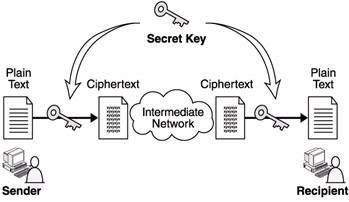
\includegraphics[scale=0.8]{../2.jpg}
\caption{Hệ mã hóa đối xứng} \label{sign1}
\end{figure}
\end{center}

Phụ thuộc vào chiều dài của khóa, có rất nhiều thuật giải mã hóa đối xứng đã được phát triển cho đến nay. Sau đây là một số thuật giải thường được sử dụng:
\begin{itemize}
\item[1. ] \textbf{Tiêu chuẩn mã hóa dữ liệu (Data Encryption Standard (DES))}. Nguyên bản DES \index{DES} đề ra giải pháp cho một khóa có chiều dài lên đến 128 bit. Tuy nhiên, kích thước của khóa đã giảm xuống còn 56 bit bởi chính phủ Hoa Kỳ trong việc nổ lực tìm ra thuật giải nhanh hơn. Việc giảm chiều dài khóa xuống, phụ thuộc vào tốc độ xử lý của bộ vi xử lý. Trong phương pháp tấn công Brute Force, các khóa sẽ phát sinh ngẩu nhiên và được gửi đến đoạn văn bản nguyên mẩu cho tới khi xác định được từ khóa chính xác. Với những khóa có kích thước nhỏ, sẽ dễ dàng để tìm ra chính xác khóa và phá vỡ hệ thống mật mã.
\item[2. ] \textbf{Bội ba tiêu chuẩn mã hóa dữ liệu (Triple Data Encryption Standard (3DES))}. Cũng giống như DES, 3DES cũng sử dụng khóa 56 bit. Tuy nhiên, nó an toàn hơn nhiều do dùng 3 khóa khác nhau để mã hóa dử liệu. Bộ xử lý thực hiện các bước sau : khóa đầu tiên dùng để mã hóa dữ liệu. Sau đó, khóa thứ hai sẽ dùng để giải mã dữ liệu vừa được mã hóa. Cuối cùng, khóa thứ ba sẽ mã hóa lần thứ hai. Toàn bộ quá trình xử lý của 3DES tạo thành một thuật giải có độ an toàn cao. Nhưng bởi vì đây là một thuật giải phức tạp nên thời gian thực hiện sẽ lâu hơn, gấp 3 lần so với phương pháp DES.
\item[3. ] \textbf{Ron's Code 4 (RC4)}. Được phát triển bởi Ron Rivest, thuật giải này sử dụng những khóa với chiều dài có thể biến đổi lên đến 256 bytes. Bởi vì chiều dài của khóa, RC4 được phân loại là một cơ chế mã hóa mạnh. Nó cũng tương đối khá nhanh. RC4 tạo một dòng bytes ngẩu nhiên và XORs chúng với văn bản nguyên mẩu. Bởi vì các bytes được phát sinh ngẩu nhiên, RC4 đòi hỏi một khóa mới cho miỗ lần gửi thông tin ra ngoài.
\end{itemize}

Do hệ mã khóa đối xứng sử dụng một khóa cho cả quá trình mã hóa và giải mã nên có các vấn đề:
\begin{itemize}
\item Khi bị lộ khóa thì tất cả các thông tin sử dụng khóa này sẽ bị huỷ. Vì thế, khóa nên thường xuyên thay đổi theo định kỳ.
\item Khi hệ thống mã hóa đồng bộ xử lý một lượng thông tin lớn, việc quả lý các khóa sẽ trở thành một công việc vô cùng khó khăn. Kết hợp với việc thiết lặp các cặp khóa, phân phối, và thay đổi theo định kỳ đều đòi hỏi thời gian và tiền bạc.
\end{itemize}

Để giải quyết các vấn đề trên hệ mã khóa công khai đã được đưa ra.
\section{Mật mã khóa công khai}
Khác với các hệ mã khóa đối xứng \index{Mã khóa đối xứng} (symmetric-key cryptography), khóa dùng giải mã và mã hóa có quan hệ rõ ràng với nhau (có thể dễ dàng tìm được một khóa nếu biết khóa kia, cả hai khóa có thể trùng nhau và đều bí mật), hệ mã khóa công khai \index{Mã khóa công khai} (public-key cryptography) có hai loại khóa là khóa bí mật và khóa công khai. Hai loại khóa này tạo thành một cặp và một loại dùng để mã hóa, loại còn lại dùng để giải mã. Đúng như cái tên người ta đặt cho hai loại khóa, khóa bí mật được giữ bí mật còn khóa công khai được công khai cho tất cả mọi người. Điểm mấu chốt trong hệ mã khóa công khai là khi biết được khóa công khai người ta không thể tìm được khóa bí mật.

Hệ mã khóa công khai cũng có thể dùng để truyền dữ liệu mà không cần phải có thao tác thống nhất khóa bí mật giữa các bên.

\begin{center}
\begin{figure}
\centering
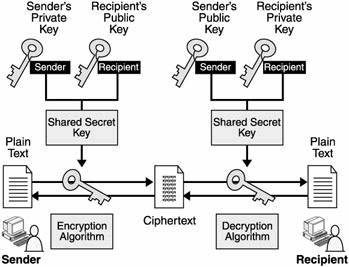
\includegraphics[width=0.6\linewidth]{../3.jpg} 
\caption{Hệ mã khóa công khai}
\end{figure}
\end{center}

\subsection*{Cơ sở toán học của thuật toán khóa công khai}
Các hệ mã khóa công khai dựa trên các hàm cửa sập (trapdoor function \index{Trapdoor function}) có đặc tính đặc biệt. Hàm $y = f(x)$ là một hàm cửa sập thì ta có thể dễ dàng tính được $y$ khi biết $x$ nhưng khi biết $y$, việc tính $x = f^{-1}(y)$ là rất khó khăn nếu không có một thông tin đặc biệt $t$. Với thông tin đặc biệt $t$ thì việc tính $x = f^{-1}(y)$ lại trở nên đơn giản. Nếu không tồn tại thông tin đặc biệt $t$, hàm này gọi là hàm cửa sập một chiều (Trapdoor one-way function). Hình \ref{trap1} mô tả cơ chế hoạt động của một hàm cửa sập.

Ví dụ: 767971435180333 là tích của hai số nguyên tố. Việc tính được số này từ tích của hai số nguyên tố là rất đơn giản nhưng để phân tích số này thành tích của hai thừa số nguyên tố ta sẽ phải thử chia nó cho tất cả các số nguyên từ hai đến $\sqrt{767971435180333}$. Đây là một bài toán khó. Tuy nhiên nếu biết được một trong hai nhân tử của nó là $p1 = 26449211$ thì việc tính nhân tử còn lại lại hết sức đơn giản. Ta chỉ việc tính $p2 = 767971435180333 \div 26449211$.

\begin{center}
\begin{figure}[H]
\centering 
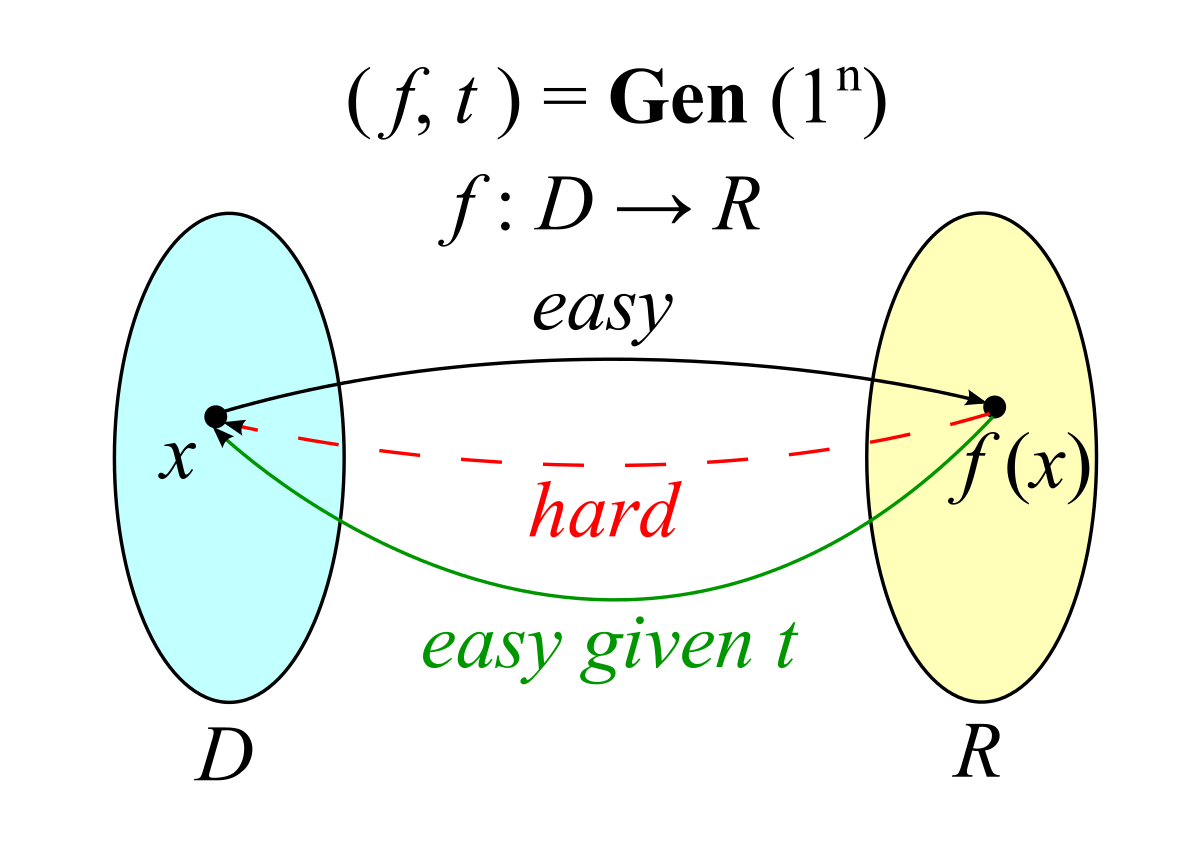
\includegraphics[width=0.6\linewidth]{../trap.png}
\caption{Trapdoor one-way function} \label{trap1}
\end{figure}
\end{center}
\subsection*{Tính an toàn}
Các hệ mã khóa công khai đòi hỏi khối lượng tính toán lớn hơn nhưng cũng không an toàn hơn so với các hệ mã khóa đối xứng. Bởi vậy người ta thường chỉ ứng dụng các hệ mã khóa công khai trong việc thống nhất khóa hoặc chuyển khóa bí mật, sau đó sẽ sử dụng các hệ mã khóa đối xứng với khóa bí mật đã thống nhất để truyền dữ liệu.
\section{Thuật toán trao đổi khóa Diffie-Hellman (DHE)}
Tương tự như các hệ mã khóa công khai, các thuật toán trao đổi khóa cũng có cơ sở toán học dựa trên một hàm cửa sập. Thuật toán trao đổi khóa khóa Diffie-Hellman  \index{Diffie-Hellman} được hai nhà khoa học Whitfield Diffie và Martin Hellman đưa ra năm 1976 và ngày nay được ứng dụng trong các giao thức truyền thông.

Trên trường đại số \index{Trường đại số} $\mathbb{Z}_p$ người ta có thể dễ dàng thực hiện phép toán $y = f(x) = g^x \ (mod \ p)$ nhưng khi biết $y$ thì việc giải ngược lại để tìm $x = log_g(y) \ (mod \ p)$ lại là một bài toán rất khó, gọi là bài toán logarithm \index{Logarithm}rời rạc. Bài toán logarithm rời rạc được sử dụng như là cơ sở toán học cho thuật toán Diffie-Hellman. \\ \\
\textbf{Thuật toán Diffie-Hellman ở dạng đơn giản}

Người ta sử dụng số nguyên tố $p$ và số $g$ là phần tử sinh của trường đại số $\mathbb{Z}_p$.
\begin{itemize}
\item[1. ] Alice và Bob cùng thống nhất với nhau chọn một số nguyên tố $p = 29$ và $g = 8$ để thực hiện việc chuyển khóa.
\item[2. ] Alice chọn một số bí mật $a = 6$ và tính g$^a \ (mod \ p)$ để gửi cho Bob: A = $8^6 \ (mod \ 23) = 13$.
\item[3. ] Bob chọn một số bí mật $b = 15$ và tính $g^b \ (mod \ p)$ để gửi cho Bob: $B = 8^{15} \ (mod \ 29) = 21$
\item[4. ] Alice tính $s = B^a \ (mod \ 29) = 21^6 \ (mod \ 29) = 13$.
\item[5. ] Bob tính $s = A^b \ (mod \ 29) = 13^{15} \ (mod \ 29) = 13$.
\end{itemize}
Từ $s = 13$ ta tìm được khóa chia sẻ mà cả hai cùng thống nhất.
\subsection*{Tính an toàn}
Thuật toán Diffie-Hellman dựa trên bài toán logarithm rời rạc, giải quyết được bài toán logarithm rời rạc đồng nghĩa với việc phá vỡ được thuật toán trao đổi khóa Diffie-Hellman.

Sau hơn 40 năm kể từ khi thuật toán trao đổi khóa Diffie-Hellman được giới thiệu, người ta đã đưa ra nhiều thuật toán để giải quyết vấn đề logarithm rời rạc. Một trong những thuật toán hiệu quả nhất phải kể đến đó là thuật toán Number Field Sieve (NFS). Để chống lại thuật toán NFS thì số nguyên tố p sử dụng trong thuật toán trao đổi khóa Diffie-Hellman phải có độ dài tối thiểu 2048 bit, tương đương với key $s$ có độ dài 2048 bit. Một số $p$ lớn như vậy đòi hỏi một khối lượng tính toán không hề nhỏ.
\section{Một số thuật toán mã khóa công khai}
\index{RSA}
\subsection*{Thuật toán RSA}
\textbf{\underline{Xây dựng}}: Chọn các tham số
\begin{itemize}
\item[1. ] \textit{Chọn hai số nguyên tố lớn p và q. Tính $n = p \times q$ và $m = \phi(n) = (p - 1) \times (q - 1)$.}
\item[2. ] \textit{Chọn e, $1 \leq e \leq m -1$, sao cho $gcd(e, m) = 1$.}
\item[3. ] \textit{Tìm d sao cho $e * d = 1$ (mod $m$), tức là tính $d = e^{-1}$
(mod $m$), giải theo thuật toán gcd mở rộng.}
\end{itemize}

\textit{Khóa công khai (Public key) là (e, n)}

\textit{Khoá dùng riêng (Private key) (là d, p, q)}

Giả sử $X$ là một khối tin gốc (plaintext), $Y$ là một khối mã tương ứng của $X$, và ($z_A, Z_A$) là các thành phần công khai và riêng của khoá của Alice

\textbf{\underline{Sinh Mã}}. Nếu Bob muốn gửi một thông báo mã hoá cho Alice thì anh ta chỉ việc dùng khoá công khai của Alice để thực hiện:
\begin{displaymath}
Y = E_{Z_A}(X) = X^e \pm n
\end{displaymath}

\textbf{\underline{Giải mã}}. Khi Alice muốn giải mã Y, cô ta chỉ việc dùng khoá riêng $z_A = d$ để thực hiện như sau:
\begin{displaymath}
D_{z_A}(Y) = Y^d \pm n
\end{displaymath}
\index{Rabin}
\subsection*{Hệ Rabin}
Hệ Rabin cũng xây dựng trên việc lấy $n=p\times q$ làm bí mật. N được coi là khoá công khai (PK) còn (p,q) là khoá bí mật (SK).

Mã hoá là việc thực hiện:
\begin{displaymath}
Y = X^2 (mod \ n)
\end{displaymath}

còn giải mã là việc tính căn bậc hai:
\begin{equation}
X = \sqrt{Y} (mod \ n)  \label{*} 
\end{equation}

Có thể thấy, nếu biết $n=p\times q$ thì dễ dàng tìm được nghiệm cho phương trình này, còn nếu không thì việc tìm nghiệm là khó tương đương với bài toán PTTSNT số n.

Khi biết $N=p\times q$ thì \ref{*} được giải ra có bốn nghiệm do đó để xác định được đâu là bản rõ gốc phải có mẹo để chọn được đúng giá trị cần thiết trong số 4 nghiệm đó

Hệ Rabin có một số ưu điểm so với RSA:
\begin{itemize}
\item Tính an toàn được chứng minh hoàn toàn tương đương với bài toán PTTSNT, nói cách khác tính ATBM của Rabin là có thể chứng minh  được (provable)
\item Ngoại trừ trường hợp RSA hoạt động với e nhỏ còn thuật toán sinh mã của Rabin nhanh hơn nhiều so với RSA là hệ đòi hỏi phải tính luỹ thừa. Thời gian giải mã thì
tương đương nhau.
\end{itemize}

Nhược điểm: Vì phương trình giải mã cho 4 nghiệm nên làm khó dễ việc giải mã. Thông thường, bản rõ trước khi được mã hoá cần được nối thêm vào đuôi một chuỗi số xác định để làm dấu vết nhận dạng (chẳng hạn nối thêm 20 số 0 – như vậy trong số 4 nghiệm giải ra, chuỗi nào tận cùng bằng 20 con 0 thì đúng là bản rõ cần nhận). Vì lý do này nên Rabin thường được dùng chủ yếu cho chứng thực (chữ ký điện tử).
\index{El-Gamal}
\subsection*{Hệ El-Gamal}
\textbf{\textit{Tạo khóa}}:

Alice chọn một số nguyên tố p và hai số nguyên ngẫu nhiên g và u, cả hai đều nhỏ hơn p. Sau đó tính 
\begin{displaymath}
y = g^u (mod \ p)
\end{displaymath}

Bây giờ khóa công khai của Alice được lấy là (p,g,y), khoá mật là u.

\textbf{\textit{Sinh mã}}:
\begin{itemize}
\item[1. ] Nếu Bob muốn mã hoá một tin $X$ để truyền cho Alice thì trước hết anh ta chọn một số ngẫu nhiên k sao cho $(k,p-1) = 1$
\item[2. ] Tính 
\begin{displaymath}
a = g^k(mod \ p)
b = y^kX(mod \ p)
\end{displaymath}
\end{itemize}

Mã là $Y = (a,b)$ và có độ dài gấp đôi bản rõ.

\textbf{\textit{Giải mã}}: Alice nhận được $Y = (a,b)$ và giải ra $X$ theo công thức sau:
\begin{displaymath}
X = \frac{b}{a^u} (mod \ p)
\end{displaymath}
\section{Chữ ký điện tử}
\index{Chữ ký điện tử}
Chữ kí điện tử là một hệ mã khóa công khai với cặp khóa $A(s_A, p_A)$ trong đó $A$ là người giữ chữ kí, $s_A$ là khóa bí mật còn $p_A$ là khóa công khai. Với một thông điệp $m$ thì người cùng $A$ sẽ kí lên thông điệp $m$ bằng cách mã hóa $m$ bởi khóa bí mật được bản mã $c_m$. Mọi người có thể kiểm tra chữ kí này có hợp lệ hay không bằng cách dùng khóa công khai để giải mã $c_m$, nếu được đúng thông điệp $m$ thì chữ kí là hợp lệ còn không, chữ kí đó không hợp lệ hay nói cách khác, người kí lên thông điệp $m$ đó không phải là A.

Chỉ có người dùng $A$ mới nắm giữ khóa bí mật $s_A$ bởi vậy chỉ có $A$ mới có khả năng kí còn tất cả mọi người đều có khóa công khai $p_A$ nên tất cả mọi người đều có khả năng kiểm tra xem một chữ kí có phải do $A$ kí hay không.

Trong thực tế, thông điệp $m$ có thể là một văn bản hay một cuốn sách, để mã hóa một khối lượng lớn dữ liệu như vậy bằng hệ mã hóa công khai sẽ rất tốn thời gian và tài nguyên hệ thống. Bởi vậy, người ta sẽ băm dữ liệu cần kí $m$ thành một chuỗi mã băm. Sau đó sẽ kí lên chuỗi mã băm đó. Thao tác xác nhận chữ kí cũng tương tự như vậy (Hình \ref{sign1}):
\subsection*{Sơ đồ chữ ký cơ bản}
\begin{center}
\begin{figure}[H] 
\centering
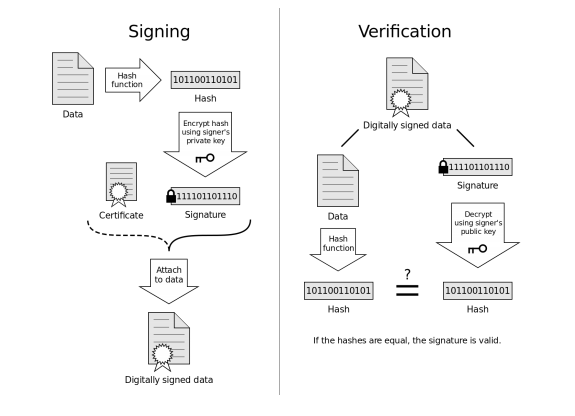
\includegraphics[width=0.8\linewidth]{../im20.png}
\caption{Quy trình thực hiện kí và xác nhận} \label{sign1}
\end{figure}
\end{center}

Trong thuật toán trao đổi khóa bí mật Diffie-Hellman \index{Diffie-Hellman} dựa trên đường cong elliptic \index{Elliptic}, kẻ tấn công xen giữa Evil có thể giả mạo là Bob khi truyền thông với Alice và giả mạo làm Bob khi truyền thông với Alice. Khi đó thuật toán sẽ được thực hiện song song giữa Evil-Alice và Evil-Bob. Dữ liệu truyền thông giữa Alice và Bob sẽ được chuyển thông qua Evil và có thể dễ dàng bị Evil giải mã. Bởi thế, người ta dùng chữ kí điện tử để xác định xem đối tượng gửi nhận dữ liệu có đúng là đối tượng mà mình mong muốn gửi nhận dữ liệu hay không.

Trong hình dưới đây, Victim là Alice, Web Server là Bob và Attacker là Evil (Hình \ref{sign2}):
\begin{center}
\begin{figure}[H] 
\centering
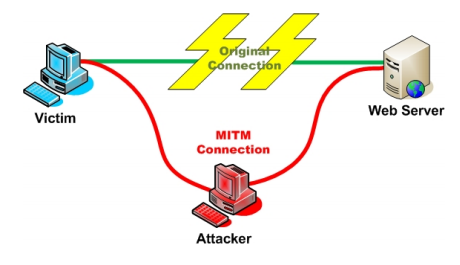
\includegraphics[width=0.65\linewidth]{../im21.png}
\caption{Tấn công Man In The Middle (nguồn: owasp) \index{Man In The Middle}} \label{sign2}
\end{figure}
\end{center}
\section{Hàm băm và ứng dụng chữ ký điện tử}
Một hàm băm \index{Hàm băm} H sẽ lấy ở đầu vào là một thông tin X có kích thước bất kỳ và sinh kết quả ra là một chuỗi $h_X=h(X)$ có độ dài cố định, thường là nhỏ hơn nhiều so với kích thước của $X$. Chuỗi này thường được gọi là cốt yếu, hay cốt (digest) của thông tin X.
\begin{center}
\begin{figure}[H]
\centering
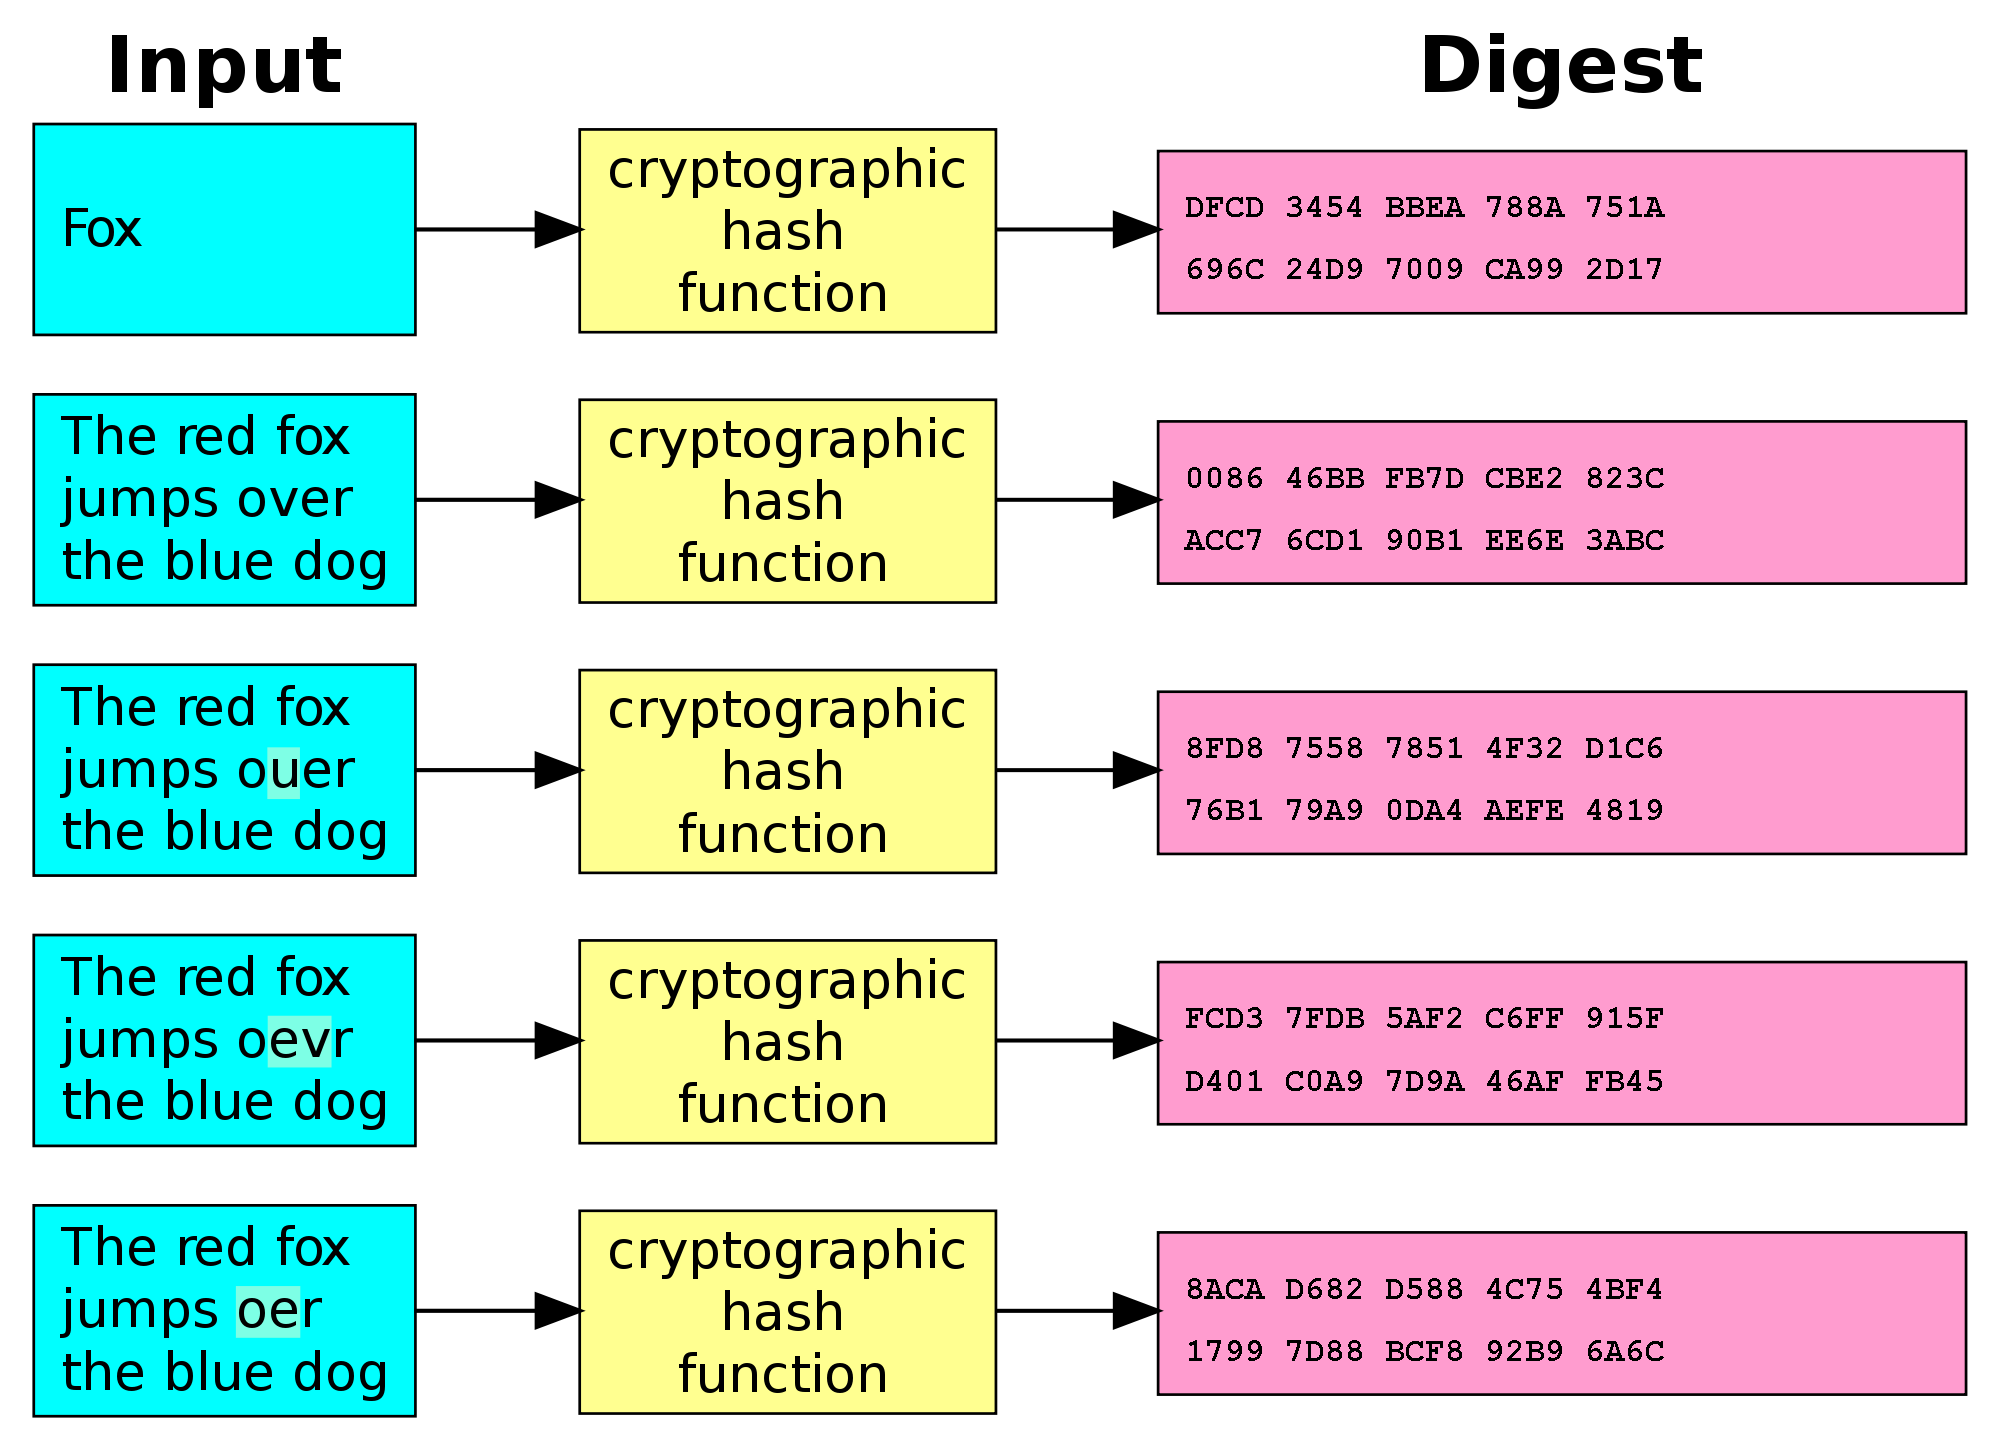
\includegraphics[width=0.65\linewidth]{../hash.png}
\caption{Hình ảnh minh họa hàm băm}
\end{figure}
\end{center}

Ví dụ: Thông tin X có thể là một tệp độ dài hàng trăm Kb trong khi cốt của nó chỉ là một khối có độ dài 128bit. Tất nhiên, điều đó dẫn đến khả năng có thể có 2 thông tin $X \neq X'$ mà cho cùng một cốt giống nhau với một hàm băm, tức là $H(X) = H(X')$. Trường hợp này gọi là đụng độ (collision \index{Collision}).

Tuy nhiên với hàm băm thiết kế tốt, đụng độ là gần như không thể xảy ra được trên thực tế. Nói cách khác nếu cố đi tìm, khối lượng tính toán phải thực hiện là rất lớn, không khả thi với công cụ tính toán hiện thời.

Hàm băm có ứng dụng chủ chốt trong các hệ chữ ký điện tử được sử dụng hiên nay. Thay vì ký (tức là thực hiện thuật toán $D_{z_A}$) lên văn bản $X$, Alice cần thực hiện việc ký lên $h_X$, như vậy văn bản đã ký sẽ có dạng $X || D_{z_A}(H(X))$.

Để đảm bảm an toàn cao, chống được tấn công giả mạo chữ ký, chúng ta cần sử dụng các hàm băm mật mã (cryptographic hash function) với các thuộc tính như sau:
\begin{itemize}
\item[1. ] Lấy đầu vào là một xâu với độ dài bất kỳ và sinh ra một xâu với độ dài cố định.
\item[2. ] Có tính một chiều: biết $X$, có thể dễ dàng tính được giá trị băm $h_X$, nhưng không thể tính ngược được $X$ khi chỉ biết $h_X$, với công cụ tính toán hiện nay (bất khả thi về tính toán).
\item[3. ] Có tính phi đụng độ cao (collision free), tức là thực tế không thể tim được hai thông tin $X \neq X'$ sao cho $H(X) = H(X')$. Tất nhiên, đây là bất khả thi về mặt tính toán.
\end{itemize}
\subsubsection{Đụng độ}
Rõ ràng là với không gian giá trị băm nhỏ hơn không gian tin về mặt kích thước thì chắc chắn sẽ tồn tại đụng độ (collision), nghĩa là có hai bản rõ $X \neq X’$ mà giá trị băm của chúng giống nhau nghĩa là $h_X=h_{X’}$. Điều này có thể thấy rõ ràng qua nguyên lý Diricle - Nếu có n+1 con thỏ được thả vào n cái chuồng thì phải tồn tại ít nhất một cái chuồng mà trong đó có ít ra là hai con thỏ ở chung.

Trong thực tế người ta thường chọn không gian băm cỡ khoảng 64bit, 128 bit \ldots .Trong khi đó các văn bản thực tế lớn hơn nhiều, cỡ Kb trở lên, cho nên việc tồn tại đụng độ là chắc chắn. Tuy nhiên nếu sử dụng hàm băm mật mã có không gian băm lớn được chế tạo tốt (an toàn) thì việc tìm ra đụng độ đòi hỏi khối lượng tính toán lớn đến mức phi thực tế (infesible computation).

Việc chế tạo các hàm băm phi đụng độ là rất khó. Nhiều hàm băm được phát minh bởi các nhóm có tên tuổi trên thế giới sau một thời gian xuất hiện đã bị những người khác chỉ ra những đụng độ tồn tại và không được công nhận là an toàn nữa.
\subsection*{Các kỹ thuật làm hàm băm}
Các kỹ thuật để chế tạo được hàm băm có thể chia ra làm ba loại:
\begin{itemize}
\item Dựa trên việc áp dụng các hệ mã khối theo mật mã khoá bí mật đối xứng (SKC).
\item Dựa trên các phép toán số học đồng dư.
\item Các hàm thiết kế băm đặc biệt.
\end{itemize}
\subsubsection{Các hàm băm chế từ hệ SKC}
\textbf{\textit{Sơ đồ Rabin-Matyas-Davies-Price (RMDP)}}
\begin{center}
\begin{tabular}{l}
$X = X_1 X_2 \ldots$ \\
$H_0 = 0$ (hay một số ngẫu nhiên nào đó) \\
$H_i = E_{x_i}(H_{i - 1})$ \\
\end{tabular}
\end{center}

Ở đây, tất nhiên các TIN phải được chặt thành các khối có kích cỡ bằng khoá của hệ mã E. Giá trị băm là $H(X) = (H_0,H_t)$.

Người ta chứng minh được rằng với không gian băm chỉ là 64bit thì $H(X)$ không phải là một chiều, tức là cho $Y=H(X)$, việc tìm ngược được X là khả thi.

\textbf{\textit{Sơ đồ Davies-Meyer (DM hash)}}
\begin{center}
\begin{tabular}{l}
$X = X_1 X_2 \ldots$ \\
$H_0 = $ vector khởi tạo là một số ngẫu nhiên nào đó \\
$H_i = E_{x_i}(H_{i-1}) \oplus H_{i-1}$	 \\
\end{tabular}
\end{center}
\begin{itemize}
\item Việc xây dựng các hàm băm từ các mã khối đòi hỏi phải có phân tích tính an toàn một cách cẩn thận.
\item DM được coi như là an toàn nếu sử dụng với các mã khối kích thước 128bit.
\item Không có hệ nào khác đã được đề xuất mà được chứng minh là an toàn.
\end{itemize}
\subsection*{Các hàm băm dựa trên các phép toán số học đồng dư}
\textbf{\textit{QCMDC (Quadratic Congruential Manipulation Detection Code)}}

Được đề xuất bởi Jueneman (1983).

Bản rõ được chia thành các khối m bit. $H_0$ là giá trị khởi đầu được chọn ngẫu nhiên và giữ bí mật (vì thế vẫn được gọi là hàm băm có khóa - keyed hash function).

Các bước xây dựng hàm băm như sau:
\begin{center}
\begin{tabular}{l}
M là một số nguyên tố sao cho $M \geq 2^{m-1}$, \\ 
$H_i = (H_i - 1 + X_i)^2$ (mod M) \\
M là luỹ thừa của 2.
\end{tabular}
\end{center}

Hệ này đã bị phá (Coppersmith).

\textbf{\textit{Davies-Price (1985)}}

Chia văn bản thành các khối có m-d bit:
\begin{center}
\begin{tabular}{l}
$X = X_1 X_2 X_3 \ldots X_n$ \\
$H_i = (H_{i-1} \oplus X_i)^2$ (mod M), $H_0 = 0$
\end{tabular}
\end{center}

Hệ này bị chứng minh là không đảm bảo tính một chiều (Girault)

\subsection*{Các hàm băm được chế tạo đặc biệt}
Ngoài các kỹ thuật thông thường nói trên người ta đã tìm nhiều cách rất riêng biệt khác nhau để chế tạo ra những hàm băm có độ tin cậy cao. Thông thường những sơ đồ này rất phức tạp và có những cấu trúc đặc biệt, nên không trình bày đầy đủ ở đây. Sau đây là một số các hàm băm nổi tiếng.
\subsubsection{MD5 \index{MD5} (Rivest 1992)}
Đây là một trong các hàm băm có tiếng nhất và được sử dụng thông dụng:
\begin{itemize}
\item[+] Nó lấy vào các khối đầu vào 512 bit và sinh ra các giá trị băm 128 bit.
\item[+] Được tin là phi đụng độ và một chiều (one - way)
\item[+] Thuật toán MD5 được thiết kế cho phép chạy tốt nhất trên các máy tính 32 bit. Nó sử dụng các phép toán đơn giản như phép cộng modulo 32, do đó thích hợp với việc mã hoá cho các bộ xử lý 32 bit.
\end{itemize}
\subsubsection{SHA \index{SHA}(Secure Hash Function)}
Đây là một thuật toán được đề xuất và bảo trợ bởi cơ quan NIST để sử dụng đối với hệ chữ ký DSA (cũng là một dự chuẩn cho chữ ký điện tử). Nó cho giá trị băm là 160 bit và được thiết kế với cùng một tiếp cận như MD5.
\subsubsection{HAVAL}
Một hệ băm của Australia cho phép thay đổi kích thước giá trị băm. Cấu trúc rất giống như MD5.
\subsubsection{Snefru Mekle (1989)}
\begin{itemize}
\item[+] Là hàm băm có khóa (keyed hash function)
\item[+] Cho phép 1 trong 2 lựa chọn kích thước giá trị băm là 128 bit và 256 bit.
\item[+] Eli Biham đã chỉ ra một đụng độ cho trường hợp 128 bit.
\end{itemize}
\section{Hệ thống chứng thực và Chứng thư số}
\index{Hệ thống chứng thực}
\index{Chứng thư số}
\subsection*{Hệ thống chứng thực}
Hệ thống chứng thực là một hạ tầng an ninh mạng được xây dựng trên một hạ tầng cơ sở khóa công khai (PKI) cung cấp các giải pháp đảm bảo an toàn cho các hoạt động (gọi chung là giao dịch) thông qua mạng.
\subsubsection{Tại sao lại phải sử dụng hệ thống chứng thực?}
\begin{itemize}
\item Hệ thống chứng thực cung cấp các dịch vụ đảm bảo an toàn cho các giao dịch thông qua mạng. Các dịch vụ cơ bản mà một hệ thống chứng thực cung cấp bao gồm:
\item Dịch vụ xác thực: nhằm xác định xem ai đang giao dịch với mình.
\item Dịch vụ bảo mật: đảm bảo tính bí mật của thông tin, người không có thẩm quyền không thể đọc được nội dung của thông tin.
\item Dịch vụ toàn vẹn: khẳng định thông tin có bị thay đổi hay không.
\item Dịch vụ chống chối bỏ: cung cấp các bằng chứng chống lại việc chối bỏ một hành động đã thực hiện hay đã diễn ra
\item Như vậy sử dụng hệ thống chứng thực sẽ đảm bảo, bí mật, toàn vẹn cho thông tin được truyền qua mạng, xác thực được người dùng và chống chối bỏ các hành động hay sự kiện đã xảy ra.
\end{itemize}
\subsubsection{Hệ thống chứng thực gồm những thành phần nào?}
\begin{itemize}
\item Hệ thống chứng thực gồm 2 thành phần:
\begin{itemize}
\item Thành phần thực hiện các nhiệm vụ về quản lý chứng thư số như: đăng ký và phát hành, thu hồi \ldots chứng thư số.
\item Thành phần thực hiện chức năng xác định xem một chứng thư số có hợp lệ hay không
\end{itemize}
\end{itemize}
\index{Cơ quan chứng thực}
\subsubsection{Cơ quan chứng thực (CA) là gì?}
Cơ quan chứng thực (Certification Authority - CA) có thẩm quyền cấp phát, thu hồi, quản lý chứng thư số cho các thực thể thực hiện các giao dịch an toàn. Cơ quan chứng thực là một thành phần chính của hệ thống chứng thực.
\index{Cơ quan đăng ký}
\subsubsection{Cơ quan đăng ký (RA) là gì?}
Cơ quan đăng ký (Registration Authority) là một thành phần trong hệ thống chứng thực có nhiệm vụ tiếp nhận và xác minh các yêu cầu về chứng thư số của người sử dụng đồng thời gửi các yêu cầu đã xác minh cho cơ quan chứng thực (CA) thực hiện yêu cầu đó.
\subsubsection{Hệ thống chứng thực có những ứng dụng gì?}
\begin{itemize}
\item Một số ứng dụng của hệ thống chứng thực:
\item Nhóm các dịch vụ chính phủ điện tử e-Government:
\begin{itemize}
\item Hóa đơn điện tử (E-Invoice)
\item Thuế điện tử (E-Tax Filing)
\item Hải quan điện tử (E-Customs)
\item Bầu cử điện tử (E-Voting)
\item E-Passport
\item PKI-based National ID Card
\item Các dịch vụ của chính phủ cho doanh nghiệp G2B (các ứng dụng đăng ký kê khai, thăm dò qua mạng đối với các doanh nghiệp)
\item  Các dịch vụ của chính phủ cho công dân G2C (dịch vụ y tế \ldots).
\end{itemize}
\item Nhóm các dịch vụ ngân hàng trực tuyến (Online Banking)
\begin{itemize}
\item Thanh toán trực tuyến (E-Payment)
\item Tiền điện tử (E-Billing)
\end{itemize}
\begin{itemize}
\item Kinh doanh chứng khoán trực tuyến (Online security trading)
\item Đấu thầu trực tuyến (E-Procurement)
\item Bảo hiểm trực tuyến (E-Insurance)
\item Quản lý tài liệu
\item Bảo mật email
\end{itemize}
\end{itemize}
\index{Chứng thư số}
\subsection*{Chứng thư số}
Để thực hiện được các giao dịch an toàn qua mạng, các bên tham gia cần phải có "chứng thư số". Chứng thư số là một cấu trúc dữ liệu chứa các thông tin cần thiết để thực hiện các giao dịch an toàn qua mạng. Chứng thư số được lưu giữ trên máy tính dưới dạng một tập tin (file).

Nội dung chứng thư số bao gồm:
\begin{itemize}
\item Tên chủ thể chứng thư số.
\item Khoá công khai.
\item Một số thông tin khác như, tên của CA cấp chứng chỉ số đó, hạn dùng, thuật toán ký \ldots.
\item Chữ ký số của CA cấp chứng thư số đó.
\end{itemize}

Mục đích của chứng thư số dùng để nhận diện một đối tượng khi tham gia giao dịch trên mạng.

\subsubsection{Ứng dụng chứng thư số để làm gì?}
\begin{itemize}
\item Với chứng thư số người dùng có thể:
\begin{itemize}
\item Xác định danh tính người dùng khi đăng nhập vào một hệ thống (xác thực).
\item Ký số các tài liệu Word, PDF hay một tệp liệu.
\item Mã hóa thông tin để đảm bảo bí mật khi gửi và nhận trên mạng.
\item Thực hiện các kênh liên lạc trao đổi thông tin bí mật với các thực thể trên mạng như thực hiện kênh liên lạc mật giữa người dùng với webserver.
\end{itemize}
\end{itemize}
%\chapter{Lý thuyết số}
%\index{logarithm}
%\index{Lý thuyết số}
%\index{Cấu trúc đại số}
%\index{Trường hữu hạn}
%Mỗi hàm cửa sập được định nghĩa trên một cấu trúc đại số. Bài toán logarithm rời rạc dựa trên đường cong elliptic cũng được định nghĩa trên một cấu trúc đại số là đường cong elliptic trên trường hữu hạn.
%\section{Nhóm}
%\index{Nhóm}
%Trong toán học, nhóm là một cấu trúc đại số bao gồm một tập hợp các phần tử cùng với phép toán hai ngôi kết hợp hai phần tử bất kỳ của tập hợp thành một phần tử thứ ba thỏa mãn bốn điều kiện gọi là tiên đề nhóm, lần lượt là tính đóng, kết hợp, phần tử đơn vị \index{Phần tử đơn vị} và tính khả nghịch.

%Cụ thể hơn, một nhóm $(G, *)$ là tập hợp các phần tử $G$ cùng với phép toán hai ngôi $*$ (hay còn gọi là luật nhóm) kết hợp thành phần tử thứ ba thỏa mãn bốn tiên đề của nhóm (với $ a, b , c, e \in G$):
%\begin{itemize}
%\item Tính đóng: $\forall a, b: (a * b) \in G$
%\item Tính kết hợp: $\forall a, b, c: (a * b) * c = a * (b * c)$
%\item Phần tử đơn vị: $\exists e \ \forall a: a * e = e * a = a$
%\item Tính khả nghịch: $\forall a \ \exists b: a * b = b * a = e$
%\end{itemize}
%$e$ được gọi là phần tử đơn vị(ví dụ nhóm số nguyên phần tử đơn vị là 0). Một nhóm được gọi là abelian \index{Abelian} khi thỏa mãn điều kiện:
%\begin{itemize}
%\item Tính giao hoán: $\forall a,b: a * b = b * a$
%\end{itemize}

%Cho $\cdot$ là phép nhân kết quả của phép cộng lặp đi lặp lại nhiều lần của 1 phần tử. Cho nhóm $(G, \cdot)$ là nhóm và $x^n$ được định nghĩa như sau:
%\begin{displaymath}
%\begin{aligned}
%x^0 & = \infty \\
%x^{n + 1} & = x^n\cdot x \ \ with \ \ n \in \mathbb{N}
%\end{aligned}
%\end{displaymath}
%$\infty$ là phép nhân phân tử đơn vị. Cấp(order) r của một phần tử x được định nghĩa như một số nguyên nhỏ r > 0 sao cho $x^r = \infty$. Nếu một nhóm có phần tử g sao cho \{$g^n | n \in Z$\} là tất cả phần tử trong nhóm, g được gọi là phần tử sinh của nhóm vòng.
%\section{Vành}
%\index{Vành}
%Một vành được gọi là nhóm abelian \index{Abelian} với phép toán hai ngôi thỏa mãn luật kết hợp và phân phối trên nhóm abelian:
%\begin{displaymath}
%\forall a, b, c \in G: a\cdot (b + c) = a \cdot b + a \cdot c
%\end{displaymath}
%\section{Trường}
%\index{Trường}
%Một trường là một vành giao hoán khác 0, chứa một nghịch đảo nhân cho mọi phần tử khác không. Như một vành, các phần tử khác không tạo thành một nhóm abelian dưới phép nhân.

%Cụ thể, cho tập $F$ và hai phép toán cộng và nhân trên $F$ thõa mãn các điều kiện:
%\begin{itemize}
%\item $F$ là nhóm giao hoán với phép cộng.
%\item $F$ là nhóm giao hoán với phép nhân.
%\item Trên $F$ phép nhân phân phối với phép cộng.
%\end{itemize}
%Hay, trong trường tập hợp $F \neq \emptyset$ trên đó xác định hai phép toán cộng và nhân:
%\begin{itemize}
%\item Phép cộng ($+$): $F \times F \rightarrow F: (a,b)\mapsto a + b$
%\item Phép nhân ($\cdot$): $F \times F \rightarrow F: (a,b)\mapsto a \cdot b$
%\end{itemize}
%Thỏa mãn các điều kiện sau:
%\begin{itemize}
%\item \textbf{Phép cộng có tính kết hợp}: $\forall a, b, c \in F, (a + b) + c = a + (b + c)$
%\item \textbf{Phép cộng có tính giao hoán}: $\forall a, b \in F, a + b = b + a$
%\item \textbf{Tồn tại phần tử 0}: $\exists 0 \in F, \forall a \in F, a + 0 = 0 + a = a$
%\item \textbf{Tồn tại phần tử đối}: $\forall a \in F, \exists (-a) \in F, a + (-a) = (-a) + a = 0$
%\item \textbf{Phép nhân có tính kết hợp}: $\forall a, b, c \in F, (a \cdot b) \cdot c = a \cdot (b \cdot c)$
%\item \textbf{Phép nhân có tính giao hoán}: $\forall a, b \in F, a \cdot b = b \cdot a$
%\item \textbf{Tồn tại phần tử đơn vị \index{Phần tử đơn vị}}: $\exists 1 \in F, 1 , 0, \forall a \in F, a \cdot 1 = 1 \cdot a = a$
%\item \textbf{Tồn tại phần tử nghịch đảo \index{Phần tử nghịch đảo}}: $\forall a \in F, a , 0, \exists a^{-1} \in F, a^{-1} \cdot a = a \cdot a^{-1} = 1$
%\item \textbf{Phép nhân phân phối với phép cộng}: $\forall a, b, c \in F, a \cdot (b + c) = a \cdot b + a \cdot c$
%\end{itemize}
%Ví dụ về trường:
%\begin{itemize}
%\item Trường số thực $(\mathbb{R})$
%\item Trường số phức $(\mathbb{C})$
%\item Trường số hữ tỉ $(\mathbb{Q})$
%\end{itemize}
%\section{Trường hữu hạn $\mathbb{F}_p$}
%\index{Trường hữu hạn}
%Chọn $p$ là một số nguyên tố. Trường hữu hạn $\mathbb{F}_q$ gọi là trường nguyên tố bao gồm một tập số nguyên $\{0, 1, 2, 3, \ldots , p - 1\}$ và những phép tính sau:
%\begin{itemize}
%\item Phép cộng: Với $a, b \in \mathbb{F}_p$ thì $a + b = r, r$ là số dư của phép chia tổng $a + b$ cho $p$. Đây gọi là phép cộng modulo, ngắn gọn hơn có thể viết $a + b = r \ (mod \ p)$.
%\item Phép nhân: Với $a, b \in \mathbb{F}_p$ thì $a \cdot b = s$, s là số dư của phép chia tích $a \cdot b$ cho $p$. Đây gọi là phép nhân modulo, ngắn gọn hơn có thể viết $a \cdot b = s \ (mod \ p)$.
%\item Phép nghịch đảo: Với $a \in \mathbb{F}_p$ và $a , 0$ thì nghịch đảo của $a, a^{-1}$là một số nguyên $x$ sao cho $a \cdot x = 1 (mod p)$
%\end{itemize}
%\subsubsection*{Ví dụ}
%Cho trường đại số hữu hạn $\mathbb{F}_p$ bao gồm tập $\mathbb{F}$ với các phần tử ${0, 1, 2, \ldots , p - 1}$. Với điều kiện $p$ ở đây là một số nguyên tố. Tập $\mathbb{F}$ như vậy kết hợp với hai phép toán cộng và nhân trên module $p$ sẽ tạo thành một trường đại số.
%\begin{itemize}
%\item[]Tập $Z$ với $p = 11: \{0, 1, 2, \ldots , 10\}$
%\item[]Phép cộng ($+$): $F \times F \rightarrow F : (a, b) \mapsto a + b \ mod \  p$
%\item[]Phép nhân ($\cdot$): $F \times F \rightarrow F : (a, b) \mapsto a \cdot b \ mod \ p$
%\begin{itemize}
%\item[*] \textbf{Phép cộng có tính kết hợp}: $\forall a, b, c \in \mathbb{F}; (a + b) + c = a + (b + c) \ (mod \ p)$
%\item[*] \textbf{Phép cộng có tính giao hoán}: $\forall a, b \in F; a + b = b + a \ (mod \ p)$
%\item[*] \textbf{Tồn tại phần tử 0}: Phần tử 0 trong trường $\mathbb{F}_p$ chính là 0. $\forall a \in F, a + 0 = 0 + a = a \ (mod \ p)$
%\item[*] \textbf{Tồn tại phần tử đối}: $\forall a \in \mathbb{F}, \exists(-a) \in F; a + (-a) = (-a) + a = 0$. Phần tử đối của a trong $\mathbb{F}_p$ chính bằng $p - a$.
%\item[*] \textbf{Phép nhân có tính kết hợp}: $\forall a, b, c \in \mathbb{F}; (a \cdot b) \cdot c = a \cdot (b \cdot c) \ (mod \ p)$
%\item[*] \textbf{Phép nhân có tính giao hoán}: $\forall a, b \in F; a \cdot b = b \cdot a (mod p)$
%\item[*] \textbf{Tồn tại phần tử đơn vị}: Phần tử đơn vị trong $\mathbb{F}_p$ chính là phần tử $1 \exists 1 \in \mathbb{F}; 1 \neq 0, \forall a \in \mathbb{F}, a \cdot 1 = 1 \cdot a = a$
%\item[*] \textbf{Tồn tại phần tử nghịch đảo}: $\forall a \in \mathbb{F}, a \neq 0, \exists a^{-1} \in \mathbb{F}; a^{-1} \cdot a = a \cdot a^{-1} = 1 \ (mod \ p)$
%\item[*] \textbf{Phép nhân phân phối với phép cộng}: $\forall a, b, c \in \mathbb{F}; a \cdot (b + c) = a \cdot b + a \cdot c \ (mod \ p)$
%\end{itemize}
%\end{itemize}
%\subsubsection*{Một số vấn đề khác}
%\begin{itemize}
%\item \textbf{Phần tử nghịch đảo \index{Phần tử nghịch đảo} và số} $p$: Việc tìm phần tử nghịch đảo chính là tìm số $b = a^{-1}$ sao cho $a \cdot b = 1 \ (mod \ p)$. Tìm phần tử nghịch đảo của 2 theo ví dụ trên ta có: $\displaystyle b = \frac{p+1}{2} = 6$ (điều kiện là $p$ là số nguyên tố). \\ \\
%Khi ước chung nhỏ nhất của $p$ và $a$ là $gcd(p, a) = 1$ thì luôn có $b, x$ để: $a \cdot b + x \cdot p = 1 \ (mod \ p)$. Khi đó $a \cdot b = 1 \ (mod \ p)$. Nghĩa là ta luôn tìm được nghịch đảo của số $a$ khi $gcd(p, a) = 1$ \\ \\
%Với $gcd(p, a) > 1$ suy ra $gcd(a \cdot b, p) > 1$ với mọi $b$ suy ra $a \cdot b , 1 \ (mod \ p)$. \\ \\
%Vậy là điều kiện để tồn tại phần tử nghịch đảo của $a$ là với mọi số nguyên $a \in {0, 1, 2, \ldots , p-1}$ thì $gcd(a, p) = 1$. Điều này đồng nghĩa với việc $p$ phải là một số nguyên tố. Hay nói cách khác $\mathbb{F}_p$ là một trường đại số nếu và chỉ nếu $p$ là một số nguyên tố.
%\item \textbf{Phần tử sinh \index{Phần tử sinh}}: Cho $g$ là một số trong trường $\mathbb{F}_p$, $g$ là phần tử sinh của $\mathbb{F}_p$ để $\{1, g, g^2, g^3, g^4, \ldots, g^{p-2}\} = Z^*$ ở đây Z được gọi là nhóm vòng \index{Nhóm vòng} và $g$ là phần tử sinh của Z. \\ \\
%Ví dụ $p = 7$ ta có $g = \{ 3^0, 3^1, 3^2, 3^3, 3^4, 3^5 \} = \{1, 3, 2, 6, 4, 5\}$. Ta có phần tử sinh là 3. Tuy nhiên không phải mọi phần tử của $Z^*$ đều là phần tử sinh.
%\end{itemize}
%\section{Truờng hữu hạn $\mathbb{F}_{2^m}$}
%Trường hữu hạn $\mathbb{F}_2^m$ gọi là một trường hữu hạn nhị phân, có thể được hiểu như một không gian vector kích thước $m$ qua trường hữu hạn $\mathbb{F}_2$ bao gồm hai phần tử 0 và 1. Nghĩa là với $m$ phần tử $\alpha_0, \alpha_1, \alpha_2, \ldots, \alpha_{m-1} \in \mathbb{F}_2^m$ và mỗi phần tử $\alpha \in \mathbb{F}_2$ $m$ có thể được viết dưới dạng:
%\begin{displaymath}
%\alpha = \alpha_0\alpha_0 + \alpha_1\alpha_1 + \ldots + \alpha_{m-1}\alpha_{m-1}	
%\end{displaymath}
%với $a_i \in \{0, 1\}$

%Tập $\alpha_0, \alpha_1, \alpha_2, \ldots, \alpha_{m-1}$ được gọi là cơ sở của $\mathbb{F}_2^m$ qua $\mathbb{F}_2$. Theo đó mỗi phần tử $\alpha \in \mathbb{F}_2^m$ đều có thể biểu diễn dưới dạng một véc tơ dạng $(a_0, a_1, a_2, \ldots, a_{m-1})$ hay là dạng chuỗi bit $a_0a_1a_2 \ldots a_{m-1}$.

%Phép toán cộng được thực hiện như là phép toán XOR hai chuỗi bit đại diện cho hai phần tử $\alpha1$ và $\alpha2$ và phép toán nhân phụ thuộc vào dạng cơ sở được chọn. Chẳng hạn như Polynomial Basis hoặc Normal Basis. Mỗi loại cơ sở sẽ hướng tới những mục đích khác nhau như hiệu quả hơn trên phần mềm hoặc phần cứng. Sau đây sẽ nói 1 số lý thuyết về dạng Polynomial Basis.
%\subsection*{Polynomial Basis}
%Gọi $f(x) = x^m + f_{m-1}x^{m-1} + \ldots + f_2x^2 + f_1x + f0 : (f_i \in {0, 1} $ với $i = 0, 1, 2, . . . , m - 1)$ là một đa thức bất khả quy bậc $m$ qua trường $\mathbb{F}_2$. Một đa thức gọi là bất khả quy có nghĩa là đa thức đó không thể phân tích thành tích của hai đa thức có bậc thấp hơn và khác không trên trường $\mathbb{F}_2$. Ví dụ như trên trường số thực, đa thức $x^2 + x + 1$ có $\delta = b^2 - 4ac = -3 < 0$ gọi là đa thức bất khả quy do không thể phân tích nó thành tích của hai nhân tử là các đa thức có bậc thấp hơn và khác không.
%\subsubsection*{Phần tử của trường}
%Trường hữu hạn $\mathbb{F}_2^m$ bao gồm tất cả các đa thức trên trường $\mathbb{F}_2$ có bậc nhỏ hơn $m$:
%\begin{displaymath}
%\mathbb{F}_2^m = a_{m-1}x^{m-1} + \ldots + a_2x^2 + a_1x + a_0 : (a_i \in \{0, 1\})
%\end{displaymath}
%Đa thức trên thường được biểu diễn ngắn gọn dưới dạng chuỗi bit độ dài $m$:
%\begin{displaymath}
%(a_{m-1}\ldots a_2a_1a_0)
%\end{displaymath}
%Hay là
%\begin{displaymath}
%\mathbb{F}_2^m = (a_{m-1}\ldots a_2a_1a_0): a_i \in \{0, 1\}
%\end{displaymath}
%Như vậy, tất cả các phần tử của $\mathbb{F}_2^m$ đều có thể biểu diễn dưới dạng chuỗi bit độ dài $m$.
%\subsubsection{Các phép toán}
%Tương tự như trường $\mathbb{F}_p$ thì trường $\mathbb{F}_2^m$ cũng có ba phép toán cơ bản sau:
%\begin{itemize}
%\item \textbf{Phép cộng}:\\
%Nếu $a = (a_{m-1} \ldots a_1a_0)$ và $b = (b_{m-1} \ldots b_1b_0)$ là các phần tử của $F_2^m$ thì $a + b = c = (c_{m-1} \ldots c_1c_0)$, với $c_i = (a_i + b_i) \ (mod \ 2)$. Đây thực chất là phép $XOR$ hai chuỗi $a$ và $b$.
%\item \textbf{Phép nhân}: \\
%Nếu $a = (a_{m-1} \ldots a_1a_0)$ và $b = (b_{m-1} \ldots b_1b_0)$ là các phần tử của $\mathbb{F}_2^m$ thì $a * b = s$ là đa thức
%\begin{displaymath}
%s_{m-1}x^{m-1} + \ldots + s_2x^2 + s_1x + s_0: s_i \in \{0, 1\}
%\end{displaymath}
%Đa thức này là kết quả của phép nhân đa thức
%\begin{displaymath}
%(a_{m-1}x^{m-1} + \ldots + a_2x^2 + a_1x + a_0) * (b_{m-1}x^{m-1} + \ldots + b_2x^2 + b_1x + b_0) \ (mod \ f(x)) (a_i, b_i \in %\{0, 1\})
%\end{displaymath}
%\item \textbf{Phép nghịch đảo}:
%Nếu $a$ là một phần tử khác 0 (phần tử bằng 0 là phần tử có tất cả các bit bằng 0) thì nghịch đảo của $a$, $a-1$ là phần tử $c \in F_2^m$ mà $a * c = 1$ (phần tử 1 là phần tử có dạng $000 \ldots 01$, tất cả các bit trừ bit cuối bằng 0).
%\end{itemize}
%\subsubsection*{Ví dụ}
%Chọn $f(x) = x^4 + x + 1$ là một đa thức tối giản, bất khả quy. Ta có 16 phần tử của trường $\mathbb{F}_2^4$ như sau:
%\begin{center}
%\begin{tabular}{rr}
%$0 (0000)$ & $x^3(1000)$ \\
%$1 (0001)$ & $x^3 + 1 (1001)$ \\
%$x (0010)$ & $x^3 + x (1010)$ \\
%$x + 1 (0011)$ & $x^3 + x + 1 (1011)$ \\
%$x^2 (0100)$ & $x^3 + x^2 (1100)$ \\
%$x^2 + 1 (0101)$ & $x^3 + x^2 + 1 (1101)$ \\
%$x^2 + x (0110)$ & $x^3 + x^2 + x (1110)$ \\
%$x^2 + x + 1 (0111)$ & $x^3 + x^2 + x + 1 (1111)$ \\
%\end{tabular}
%\end{center}
%Theo đó, một vài phép toán được thực hiện như sau:
%\begin{itemize}
%\item[-] Phép cộng: $(1101) + (1001) = (0100)$ ($XOR$ hai chuỗi)
%\item[-] Phép nhân: $(1101) * (1001) = (1111)$ Cụ thể hơn:
%\begin{displaymath}
%\begin{split}
%(x^3 + x^2 + 1) * (x^3 + 1) & = x^6 + x^3 + x^5 + x^2 + x^3 + 1 \\
%							& = x^6 + x^5 + 2x^3 + x^2 + 1 \\
%							& = x^6 + x^5 + x^2 + 1 \ (\ \mathbb{F}_2^m \ )
%\end{split}
%\end{displaymath}
%Lại có: $x^6 + x^5 + 2x^3 + x^2 + 1 mod (x^4 + x + 1) = 3x^3 + x^2 + x + 1(1111)$
%\item[-]  Phép nghịch đảo: $(1101)^{-1} = (0100)$
%\end{itemize}
%Tương tự như trường $\mathbb{F}_p$, trường $\mathbb{F}_2^m$ cũng có phần tử gọi là phần tử sinh. Trong ví dụ trên, phần tử $%\alpha = x = (0010)$ là phần tử sinh của $F_2^4$.
%\begin{center}
%\begin{tabular}{lr}
%$\alpha^1 = (0010)$ & $\alpha^9 = (1010)$ \\
%$\alpha^2 = (0100)$ & $\alpha^{10} = (0111)$ \\
%$\alpha^3 = (1000)$ & $\alpha^{11} = (1110)$ \\
%$\alpha^4 = (0011)$ & $\alpha^{12} = (1111)$ \\ 
%$\alpha^5 = (0110)$ & $\alpha^{13} = (1101)$ \\
%$\alpha^6 = (1100)$ & $\alpha^{14} = (1001)$ \\
%$\alpha^7 = (1011)$ & $\alpha^{15} = (0001)$ \\
%$\alpha^8 = (0101)$ & 
%\end{tabular}
%\end{center}
\chapter{Mật mã dựa trên đường cong Elliptic}
\section{Lý thuyết số}
\index{logarithm}
\index{Lý thuyết số}
\index{Cấu trúc đại số}
\index{Trường hữu hạn}
Mỗi hàm cửa sập được định nghĩa trên một cấu trúc đại số. Bài toán logarithm \index{Logarithm}rời rạc dựa trên đường cong elliptic cũng được định nghĩa trên một cấu trúc đại số là đường cong elliptic trên
trường hữu hạn.
\subsection*{Nhóm}
\index{Nhóm}
Trong toán học, nhóm là một cấu trúc đại số bao gồm một tập hợp các phần tử cùng với phép toán hai ngôi kết hợp hai phần tử bất kỳ của tập hợp thành một phần tử thứ ba thỏa mãn bốn điều kiện gọi là tiên đề nhóm, lần lượt là tính đóng, kết hợp, phần tử đơn vị \index{Phần tử đơn vị} và tính khả nghịch.

Cụ thể hơn, một nhóm $(G, *)$ là tập hợp các phần tử $G$ cùng với phép toán hai ngôi $*$ (hay còn gọi là luật nhóm) kết hợp thành phần tử thứ ba thỏa mãn bốn tiên đề của nhóm (với $ a, b , c, e \in G$):
\begin{itemize}
\item Tính đóng: $\forall a, b: (a * b) \in G$
\item Tính kết hợp: $\forall a, b, c: (a * b) * c = a * (b * c)$
\item Phần tử đơn vị: $\exists e \ \forall a: a * e = e * a = a$
\item Tính khả nghịch: $\forall a \ \exists b: a * b = b * a = e$
\end{itemize}
$e$ được gọi là phần tử đơn vị(ví dụ nhóm số nguyên phần tử đơn vị là 0). Một nhóm được gọi là abelian \index{Abelian} khi thỏa mãn điều kiện:
\begin{itemize}
\item Tính giao hoán: $\forall a,b: a * b = b * a$
\end{itemize}

Cho $\cdot$ là phép nhân kết quả của phép cộng lặp đi lặp lại nhiều lần của 1 phần tử. Cho nhóm $(G, \cdot)$ là nhóm và $x^n$ được định nghĩa như sau:
\begin{displaymath}
\begin{aligned}
x^0 & = \infty \\
x^{n + 1} & = x^n\cdot x \ \ with \ \ n \in \mathbb{N}
\end{aligned}
\end{displaymath}
$\infty$ là phép nhân phân tử đơn vị. Cấp(order) r của một phần tử x được định nghĩa như một số nguyên nhỏ r > 0 sao cho $x^r = \infty$. Nếu một nhóm có phần tử g sao cho \{$g^n | n \in Z$\} là tất cả phần tử trong nhóm, g được gọi là phần tử sinh của nhóm vòng.
\subsection*{Vành}
\index{Vành}
Một vành được gọi là nhóm abelian \index{Abelian} với phép toán hai ngôi thỏa mãn luật kết hợp và phân phối trên nhóm abelian:
\begin{displaymath}
\forall a, b, c \in G: a\cdot (b + c) = a \cdot b + a \cdot c
\end{displaymath}
\subsection*{Trường}
\index{Trường}
Một trường là một vành giao hoán khác 0, chứa một nghịch đảo nhân cho mọi phần tử khác không. Như một vành, các phần tử khác không tạo thành một nhóm abelian dưới phép nhân.

Cụ thể, cho tập $F$ và hai phép toán cộng và nhân trên $F$ thõa mãn các điều kiện:
\begin{itemize}
\item $F$ là nhóm giao hoán với phép cộng.
\item $F$ là nhóm giao hoán với phép nhân.
\item Trên $F$ phép nhân phân phối với phép cộng.
\end{itemize}
Hay, trong trường tập hợp $F \neq \emptyset$ trên đó xác định hai phép toán cộng và nhân:
\begin{itemize}
\item Phép cộng ($+$): $F \times F \rightarrow F: (a,b)\mapsto a + b$
\item Phép nhân ($\cdot$): $F \times F \rightarrow F: (a,b)\mapsto a \cdot b$
\end{itemize}
Thỏa mãn các điều kiện sau:
\begin{itemize}
\item \textbf{Phép cộng có tính kết hợp}: $\forall a, b, c \in F, (a + b) + c = a + (b + c)$
\item \textbf{Phép cộng có tính giao hoán}: $\forall a, b \in F, a + b = b + a$
\item \textbf{Tồn tại phần tử 0}: $\exists 0 \in F, \forall a \in F, a + 0 = 0 + a = a$
\item \textbf{Tồn tại phần tử đối}: $\forall a \in F, \exists (-a) \in F, a + (-a) = (-a) + a = 0$
\item \textbf{Phép nhân có tính kết hợp}: $\forall a, b, c \in F, (a \cdot b) \cdot c = a \cdot (b \cdot c)$
\item \textbf{Phép nhân có tính giao hoán}: $\forall a, b \in F, a \cdot b = b \cdot a$
\item \textbf{Tồn tại phần tử đơn vị \index{Phần tử đơn vị}}: $\exists 1 \in F, 1 , 0, \forall a \in F, a \cdot 1 = 1 \cdot a = a$
\item \textbf{Tồn tại phần tử nghịch đảo \index{Phần tử nghịch đảo}}: $\forall a \in F, a , 0, \exists a^{-1} \in F, a^{-1} \cdot a = a \cdot a^{-1} = 1$
\item \textbf{Phép nhân phân phối với phép cộng}: $\forall a, b, c \in F, a \cdot (b + c) = a \cdot b + a \cdot c$
\end{itemize}
Ví dụ về trường:
\begin{itemize}
\item Trường số thực $(\mathbb{R})$
\item Trường số phức $(\mathbb{C})$
\item Trường số hữ tỉ $(\mathbb{Q})$
\end{itemize}
\subsection*{Trường hữu hạn $\mathbb{F}_p$}
\index{Trường hữu hạn}
Chọn $p$ là một số nguyên tố. Trường hữu hạn $\mathbb{F}_q$ gọi là trường nguyên tố bao gồm một tập số nguyên $\{0, 1, 2, 3, \ldots , p - 1\}$ và những phép tính sau:
\begin{itemize}
\item Phép cộng: Với $a, b \in \mathbb{F}_p$ thì $a + b = r, r$ là số dư của phép chia tổng $a + b$ cho $p$. Đây gọi là phép cộng modulo, ngắn gọn hơn có thể viết $a + b = r \ (mod \ p)$.
\item Phép nhân: Với $a, b \in \mathbb{F}_p$ thì $a \cdot b = s$, s là số dư của phép chia tích $a \cdot b$ cho $p$. Đây gọi là phép nhân modulo, ngắn gọn hơn có thể viết $a \cdot b = s \ (mod \ p)$.
\item Phép nghịch đảo: Với $a \in \mathbb{F}_p$ và $a , 0$ thì nghịch đảo của $a, a^{-1}$là một số nguyên $x$ sao cho $a \cdot x = 1 (mod p)$
\end{itemize}
\subsubsection*{Ví dụ}
Cho trường đại số hữu hạn $\mathbb{F}_p$ bao gồm tập $\mathbb{F}$ với các phần tử ${0, 1, 2, \ldots , p - 1}$. Với điều kiện $p$ ở đây là một số nguyên tố. Tập $\mathbb{F}$ như vậy kết hợp với hai phép toán cộng và nhân trên module $p$ sẽ tạo thành một trường đại số.
\begin{itemize}
\item[]Tập $Z$ với $p = 11: \{0, 1, 2, \ldots , 10\}$
\item[]Phép cộng ($+$): $F \times F \rightarrow F : (a, b) \mapsto a + b \ mod \  p$
\item[]Phép nhân ($\cdot$): $F \times F \rightarrow F : (a, b) \mapsto a \cdot b \ mod \ p$
\begin{itemize}
\item[*] \textbf{Phép cộng có tính kết hợp}: $\forall a, b, c \in \mathbb{F}; (a + b) + c = a + (b + c) \ (mod \ p)$
\item[*] \textbf{Phép cộng có tính giao hoán}: $\forall a, b \in F; a + b = b + a \ (mod \ p)$
\item[*] \textbf{Tồn tại phần tử 0}: Phần tử 0 trong trường $\mathbb{F}_p$ chính là 0. $\forall a \in F, a + 0 = 0 + a = a \ (mod \ p)$
\item[*] \textbf{Tồn tại phần tử đối}: $\forall a \in \mathbb{F}, \exists(-a) \in F; a + (-a) = (-a) + a = 0$. Phần tử đối của a trong $\mathbb{F}_p$ chính bằng $p - a$.
\item[*] \textbf{Phép nhân có tính kết hợp}: $\forall a, b, c \in \mathbb{F}; (a \cdot b) \cdot c = a \cdot (b \cdot c) \ (mod \ p)$
\item[*] \textbf{Phép nhân có tính giao hoán}: $\forall a, b \in F; a \cdot b = b \cdot a (mod p)$
\item[*] \textbf{Tồn tại phần tử đơn vị}: Phần tử đơn vị trong $\mathbb{F}_p$ chính là phần tử $1 \exists 1 \in \mathbb{F}; 1 \neq 0, \forall a \in \mathbb{F}, a \cdot 1 = 1 \cdot a = a$
\item[*] \textbf{Tồn tại phần tử nghịch đảo}: $\forall a \in \mathbb{F}, a \neq 0, \exists a^{-1} \in \mathbb{F}; a^{-1} \cdot a = a \cdot a^{-1} = 1 \ (mod \ p)$
\item[*] \textbf{Phép nhân phân phối với phép cộng}: $\forall a, b, c \in \mathbb{F}; a \cdot (b + c) = a \cdot b + a \cdot c \ (mod \ p)$
\end{itemize}
\end{itemize}
\subsection*{Một số vấn đề khác}
\begin{itemize}
\item \textbf{Phần tử nghịch đảo \index{Phần tử nghịch đảo} và số} $p$: Việc tìm phần tử nghịch đảo chính là tìm số $b = a^{-1}$ sao cho $a \cdot b = 1 \ (mod \ p)$. Tìm phần tử nghịch đảo của 2 theo ví dụ trên ta có: $\displaystyle b = \frac{p+1}{2} = 6$ (điều kiện là $p$ là số nguyên tố). \\ \\
Khi ước chung nhỏ nhất của $p$ và $a$ là $gcd(p, a) = 1$ thì luôn có $b, x$ để: $a \cdot b + x \cdot p = 1 \ (mod \ p)$. Khi đó $a \cdot b = 1 \ (mod \ p)$. Nghĩa là ta luôn tìm được nghịch đảo của số $a$ khi $gcd(p, a) = 1$ \\ \\
Với $gcd(p, a) > 1$ suy ra $gcd(a \cdot b, p) > 1$ với mọi $b$ suy ra $a \cdot b , 1 \ (mod \ p)$. \\ \\
Vậy là điều kiện để tồn tại phần tử nghịch đảo của $a$ là với mọi số nguyên $a \in \{0, 1, 2, \ldots , p-1 \}$ thì $gcd(a, p) = 1$. Điều này đồng nghĩa với việc $p$ phải là một số nguyên tố. Hay nói cách khác $\mathbb{F}_p$ là một trường đại số nếu và chỉ nếu $p$ là một số nguyên tố.
\item \textbf{Phần tử sinh \index{Phần tử sinh}}: Cho $g$ là một số trong trường $\mathbb{F}_p$, $g$ là phần tử sinh của $\mathbb{F}_p$ để $\{1, g, g^2, g^3, g^4, \ldots, g^{p-2}\} = Z^*$ ở đây Z được gọi là nhóm vòng \index{Nhóm vòng} và $g$ là phần tử sinh của Z. \\ \\
Ví dụ $p = 7$ ta có $g = \{ 3^0, 3^1, 3^2, 3^3, 3^4, 3^5 \} = \{1, 3, 2, 6, 4, 5\}$. Ta có phần tử sinh là 3. Tuy nhiên không phải mọi phần tử của $Z^*$ đều là phần tử sinh.
\end{itemize}
\section{Đường cong Elliptic}
\index{Đường cong Elliptic}
Một đường cong elliptic curve được xác định bởi phương trình đường cong và một số trường tọa độ cơ bản.

Tất cả tọa độ thỏa mãn phương trình đường cong sẽ tạo thành một đường cong $E$. Tọa độ là cặp các phần tử trong trường hữu hạn. Phương trình đường cong phụ thuộc vào việc lựa chọn hệ tọa độ cực (mặc định thường là hệ tọa độ affine). Đường cong elliptic có một số luât quan trong. Luật cộng (add) cho phép cộng hai điểm trên đường cong. Luật doubling cho phép nhân một điểm trên đường cong với 2. Luật nhân cho phép nhân một điểm trên đường cong với một số (hay cộng nhiều lần điểm đấy với chính nó). Mọi đường cong đều có điểm đơn vị định nghĩa là $\infty$. Nó có xác định luật cộng riêng.

$E(GF(p^k))$ là tập hợp các điểm thỏa mãn phương trình đường cong (và cả điểm $\infty$). Lực lượng $|E(GF(p^k))|$ được định nghĩa là cấp (order) của đường cong. Nếu muốn xác định một số phần tử của 
$E(GF(p^k))$ như một điểm sinh. Nó tạo ra nhóm con khác theo luật:
\begin{displaymath}
h = \frac{|E(GF(p^k))|}{o}
\end{displaymath}
h được gọi là cofactor và o được gọi là cấp(order) của điểm sinh.

Số lượng điểm sinh của trường $GF(n)$ là $\phi (n - 1)$ ở đây $\phi$ là một hàm Ơ-le của Euler. Điều này cũng là yếu tố cho phép nhân trong nhóm vòng[*].

Đường cong elliptic có một số phương trình đường như \textit{Weierstrass Curve \index{Weierstrass Curve}, Montgomery Curve \index{Montgomery Curve}, Edwards Curve \index{Edwards Curve}, Twisted Edwards Curve \index{Twisted Edwards Curve}, \ldots } chúng ta sẽ xem xét các luật cộng, doubling, nhân và các tính chất của các luật của các đường cong ở phần tiếp theo.
\subsection*{Luật cộng}
\index{Luật cộng}
Một đường cong elliptic là tập hợp các nghiệm của phương trình:
\begin{displaymath}
Y^2 = X^3 + AX + B.
\end{displaymath}

Phương trình này được gọi là phương trình Weierstrass. Ta có hai ví dụ về đường cong elliptic

\begin{center}
\begin{tabular}{ccc}
$E_1: Y^2 = X^3 - 3X + 3$ & và & $E_2: Y^2 = X^3 - 6X + 5$ 
\end{tabular}
\end{center}
\begin{figure}[h]
\begin{center}
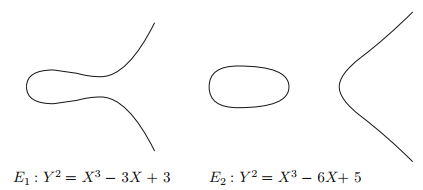
\includegraphics[scale=0.95]{../im1.png} \label{h2.1}  \refstepcounter{someCounter}
\caption{Hai ví dụ minh họa về đường cong elliptic}
\end{center}
\end{figure}
Một đặc điểm của đường cong elliptic là lấy hai điểm bất kì trên đường cong và cộng chúng lại để tạo ra một điểm thứ ba nằm trên đường cong. Nhưng không giống như luật cộng thông thường chúng ta sẽ mô tả luật cộng thông qua hình học.
\begin{figure}[h]
\begin{center}
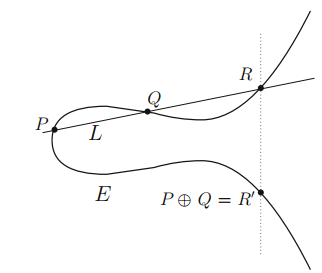
\includegraphics[scale=1=0.95]{../im2.png}
\refstepcounter{someCounter}
\caption{Luật cộng trên đường cong elliptic}
\label{fig:h2.2}
\end{center}
\end{figure}

Cho $P$ và $Q$ là hai điểm trên đường cong elliptic $E$, như hình \ref{fig:h2.2}. Kẻ đường thẳng $L$ đi qua $P$ và $Q$. Đường thẳng $L$ cắt đường cong $E$ tại ba điểm, trong đố có hai điểm $P$ và $Q$ và một điểm khác là $R$. Chúng ta lấy điểm $R$ và chiếu nó theo chục x để lấy được điểm mới $R'$. Điểm $R'$ được gọi là "tổng của $P$ và $Q$", có thể thấy phép cộng này không giống như các phép cộng thông thường. Chúng ta có thể kí hiệu phép cộng bởi $\oplus$.
\begin{displaymath}
P \oplus Q = R'
\end{displaymath}

Một ví dụ về luật cộng. Cho đường cong $E$ có phương trình:
\begin{equation}
Y^2 = X^3 - 15X + 18 \label{2.1}
\end{equation}

Cho hai điểm $P = (7,16)$ và $Q = (1,2)$ nằm trên đường cong $E$. Đường thẳng $L$ đi qua hai điểm có phương trình:
\begin{equation}
L: Y = \frac{7}{3} - \frac{1}{3} \label{2.2}
\end{equation}
Để tìm được giao điểm của đường thẳng $L$ và đường cong $E$. Chúng ta sẽ thay phương trình \ref{2.2} vào \ref{2.1} Ta có:
\begin{displaymath}
\begin{aligned}
(\frac{7}{3}X - \frac{1}{3})^2 & = X^3 - 15X + 18, \\
\frac{49}{9}X^2 - \frac{14}{9}X + \frac{1}{9} & = X^3 - 15X + 18, \\
0 & = X^3 - \frac{49}{9}X^2 - \frac{121}{9}X + \frac{161}{9}
\end{aligned}
\end{displaymath}
Chúng ta cần tìm nghiệm của đa thức. Nhìn chung để tìm nghiệm của đa thức là khó. Tuy nhiên như chúng ta đã biết $L \cap E$ Tại hai điểm P và Q nên ta có hai là $X = 7$ và $X = 1$,vì thế chúng ta có thể dễ dàng tìm được nghiệm thứ ba còn lại:
\begin{displaymath}
X^3 - \frac{49}{9}X^2 - \frac{121}{9}X + \frac{161}{9} = (X - 7)\cdot(X - 1)\cdot(X + \frac{23}{9})
\end{displaymath}
vì vậy điểm thứ ba là giao điểm của $L$ và $E$ sẽ có tọa $\displaystyle X = -\frac{23}{9}$. Chúng ta sẽ tìm tọa đô Y theo X bằng cách thay X vào phương trình \ref{2.2} kết quả $\displaystyle R = (-\frac{23}{9}, -\frac{170}{27})$. Cuối cùng chúng ta sẽ chiếu $R$ theo chục tọa đô X đạt được 
\begin{displaymath}
P \oplus Q = (-\frac{23}{9}, \frac{170}{27}).
\end{displaymath} 

\begin{figure}[h] 
\begin{center}
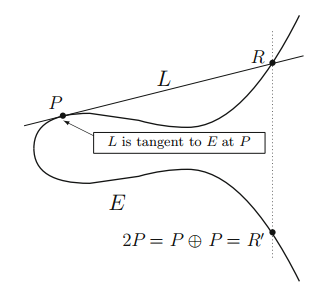
\includegraphics[scale=1]{../im3.png}
\caption{Cộng điểm P với chính nó} \label{h2.3}
\end{center}
\end{figure}

Có một số vấn đề, đầu tiên ta có thể nhìn thấy trong hình \ref{fig:h2.2} nếu như $Q$ tiệm cận đến $P$ hay nói các khác là ta thực hiện phép cộng điểm $P$ với chính nó. Khi đó đường thẳng $L$ trở thành tiếp tuyến của $E$ tại $P$ thấy hình \ref{h2.3}. Do đó việc thực hiện phép cộng điểm $P$ với chính nó chúng ta chỉ đơn gian là kéo dài tiếp tuyến $L$ tại $P$ cắt $E$ tại $P$ và một điểm còn lại là $R$ và chúng ta vẫn xử lý như trước. Theo một nghĩa nào đó $L$ vẫn cắt $E$ tại 3 điểm nhưng điểm $P$ được tính là hai.

Ví dụ tiếp tục với đường cong E với phương trình \ref{2.1} và điểm P ở ví dụ trên, chúng ta sẽ tính $P \oplus P$ hệ số góc tiếp tuyến của $E$ ở $P$ được tính bởi đạo hàm phương trình \ref{2.1}. Do đó ta có:
\begin{displaymath}
2Y\frac{dY}{dX} = 3X^2 - 15 \Rightarrow \frac{dY}{dX} = \frac{3X^2 - 15}{2Y}
\end{displaymath}
Thay tọa độ điểm $P = (7,16)$ vào ta được hệ số góc $\displaystyle \lambda = \frac{33}{8}$ và đường thẳng tiếp tuyến với $E$ tại $P$ có phương trình
\begin{equation}
L: Y = \frac{33}{8}X - \frac{103}{8} \label{2.3}
\end{equation}
Từ \ref{2.3} và \ref{2.1} ta có:
\begin{displaymath}
\begin{aligned}
(\frac{33}{8}X - \frac{103}{8})^2 & = X^3 - 15X + 18, \\
X^3 - \frac{1089}{64}X^2 + \frac{2919}{32}X - \frac{9457}{64} & = 0, \\
(X - 7)^2\cdot(X - \frac{193}{64}) & = 0.
\end{aligned}
\end{displaymath}
Tọa độ $X$ của điểm P là nghiệm kép của phương trình ta dễ dàng tìm được nghiệm còn lại $\displaystyle X = \frac{193}{64}$, thay $X$ vào \ref{2.3} tìm được $\displaystyle Y = -\frac{223}{512}$.Từ đó ta thu được kết quả của phép cộng
\begin{displaymath}
P \oplus P = (\frac{193}{64}, \frac{223}{512}).
\end{displaymath}

\begin{figure}[h]
\begin{center}
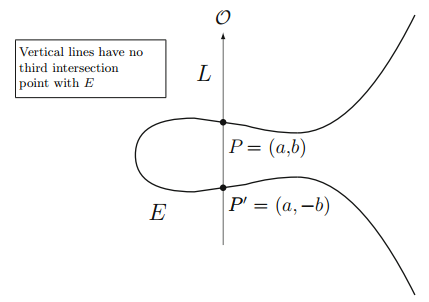
\includegraphics[scale=1]{../im4.png}
\refstepcounter{someCounter}
\caption{Đường thẳng đứng $L$ đi qua $P = (a, b)$ và $P' = (a, -b)$}
\label{h2.4}
\end{center}
\end{figure}

Vấn đề thứ hai với luật cộng phát sinh là nếu như chúng ta cộng điểm $P = (a, b)$ với điẻm đối của nó  $P' = (a, -b)$ đường thẳng đi qua $P$ và $P'$ là x = a và nó chỉ cắt đường cong tại 2 điểm $P$ và $P'$(hình \ref{h2.4}) không có điểm thứ ba xuất hiện chúng ta sẽ thêm một điểm $\mathcal{O}$ nằm ở vô cùng và điểm này không tồn tại trong mặt phẳng XY, chúng ta giả định nó luôn nằm trên đường thẳng dọc và chúng ta sẽ xét phép cộng như sau
\begin{displaymath}
P \oplus P' = \mathcal{O}.
\end{displaymath}

Nếu công điểm $\mathcal{O}$ với điểm $P$ nằm trên E sẽ như nào? Đường thẳng $L$ đi qua $\mathcal{O}$ và $P$ là đường theo chiều dọc đi qua $P$ khi đó $\mathcal{O}$ nằm trên đường dọc này và đường thẳng sẽ cắt $E$ tại điểm $P$, $\mathcal{O}$ và điểm $P' = (a , -b)$. Nên phép công $P$ với $\mathcal{O}$, chúng ta lấy hình chiếu của $P'$ qua trục X sẽ thu được điểm $P$ ban đầu. Nói một các khác $P \oplus \mathcal{O} = P$, vì vậy $\mathcal{O}$ giống như số không trong phép cộng của đường cong elliptic

Qua đây có một số định nghĩa về đường cong elliptic
\\[6pt]
\begin{definition}
Một đường cong $E$ là tập các nghiệm của phương trình Weierstrass
\begin{displaymath}
E: Y^2 = X^3 + AX + B,
\end{displaymath}
cùng với điểm $O$, với hằng số A, B thỏa mãn điều kiện
\begin{displaymath}
4A^3 + 27B^2 \neq 0,
\end{displaymath}
\end{definition}

Luật cộng trên $E$ được định nghĩa như sau. Cho $P$ và $Q$ là hai điểm trên $E$. Cho $L$ là đường thẳng qua $P$ và $Q$, hoặc là tiếp tuyến của $E$ tại $P$ nếu như $P = Q$. Giao điểm của $E$ và $L$ có chứa ba điểm $P, Q, R$ phép cộng sẽ được tính thích hợp với điểm $\mathcal{O}$ nằm trên đường dọc vô cùng. Điểm $R = (a, b)$, tổng của $P$ và $Q$ được định nghĩa là $R' = (a, -b)$ hình chiếu của $R$ qua trục X. Tổng này được định nghĩa là $P \oplus Q$ hay đơn gian hơn là $P + Q$.

Hơn nữa, nếu $P = (a, b)$ chúng ta định nghĩa điểm đối $-P = (a, -b)$, chúng ta định nghĩa $P - Q$ trở thành $P + (-Q)$. Tương tự phép cộng lặp nhiều lần được biểu diễn như phép nhân một điểm với một số nguyên,
\begin{displaymath}
nP = \underbrace{P + P + P + \ldots + P}_{n}.
\end{displaymath}
\begin{theorem} \label{dl2.1}
Cho đường cong $E$. Luật cộng \index{Luật cộng} trên đường cong $E$ thỏa mãn tính chất:
\begin{itemize}
\item[(a)] $P + \mathcal{O} = \mathcal{O} + P = P \ \forall P \in E$ (phần tử đơn vị)
\item[(b)] $P + (-P) = \mathcal{O} \ \forall P \in E$ (phần tử nghịch)
\item[(c)] $(P + Q) + R = P + (Q + R) \ \forall P, Q, R \in E$ (kết hợp)
\item[(d)] $P + Q = Q + P \ \forall P, Q \in E$ (giao hoán) 
\end{itemize}
Hay nói cách khách tập các điểm thuôc $E$ với luật cộng tạo thành nhóm abelian
\end{theorem}
\begin{theorem} \label{dl2.2}
Thuật toán Cộng trên đường cong elliptic với phương trình đường cong Weierstrass. Cho
\begin{displaymath}
E: Y^2 = X^3 + AX + B
\end{displaymath}
là một đường cong elliptic và hai điểm $P_1$ và $P_2$ nằm trên đường cong $E$.
\begin{itemize}
\item[(a)] Nếu $P_1 = \mathcal{O}$ thì $P_1 + P_2 = P_2$.
\item[(b)] trái lại $P_2 = \mathcal{O}$ thì $P_1 + P_2 = P_1$.
\item[(c)] trái lại $P_1 = (x_1, y_1)$ và $P_2 = (x_2, y_2)$
\item[(d)] nếu $x_1 = x_2$ và $y_1 = -y_2$ thì $P_1 + P_2 = \mathcal{O}$.
\item[(e)] trái lại, định nghĩa $\lambda$ bằng
\begin{displaymath}
\lambda = \left\{ \begin{array}{ll}
\displaystyle \frac{y_2 - y_1}{x_2 - x_1} & if \ P_1 \neq P_2  \\
\\
\displaystyle \frac{3x_1^2 + A}{2y_1} & if \ P_1 = P_2,
\end{array} \right.
\end{displaymath}
và
\begin{displaymath}
x_3 = \lambda^2 - x_1 - x_2 \ \ \& \ \ y_3 = \lambda(x_1 - x_3) - y_1
\end{displaymath}
Phép cộng $P_1 + P_2 = (x_3,y_3)$
\end{itemize}
\end{theorem}
\subsection*{Đường cong Elliptic trên trường hữu hạn}
\index{Đường cong Elliptic trên trường hữu hạn}
Trong phần trước chúng ta đã xem xét lí thuyết về đường cong bằng hình học. Ví dụ tổng của hai điểm phân biệt $P$ và $Q$ trên đường cong $E$ được định nghĩa bởi đường thẳng $L$ đi qua hai điểm $P$ và $Q$ sau đó tìm điểm thứ ba là giao điểm của $L$ và $E$ như minh hoa ở trên. Tuy nhiên để áp dụng lí thuyết elliptic vào mật mã, chúng ta cần nhìn đường cong và các điểm của nó có tọa độ nằm trong trường hữu hạn $\mathbb{F}_p$ điều này dễ làm.
\begin{definition}
Cho $p$ $\geq$ 3 là một số nguyên tố. Một đường cong elliptic trên trường $\mathbb{F}_p$ có công thức
\begin{center}
$E: Y^2 = X^3 + AX + B$ với $A, B \in F_p$ thỏa mãn $47A^3 + 27B^2 \neq  0$.
\end{center} 
Với tập các điểm trên E với tọa độ nằm trong trường $\mathbb{F}_p$
\begin{center}
$E(\mathbb{F}_p) = \{ (x, y): x, y \in \mathbb{F}_p$ thỏa mãn $y^2 = x^3 + Ax + B \} \cup \{ O \}$
\end{center}
\end{definition}
Xem xét ví dụ với đường cong elliptic
\begin{center}
$E: y^2 = x^3 + 3x + 8$ trên trường $\mathbb{F}_{29}$
\end{center}
Với công thức trên $a = 3$ và $b = 8$ thỏa mãn $47A^3 + 27B^2 \neq  0$ (mod 29).


Chúng ta có thể tìm thấy các điểm của $E(\mathbb{F}_{29})$ bằng các thay lần lượt các giá trị của $X = 0, 1, 2, \ldots, 28$ và kiểm tra với giá trị $X$ kết quả của phương trình $x^3 + 3x + 8$ có phải là một bình phương với modulo 29 không.
\begin{center}
\begin{figure}[h]
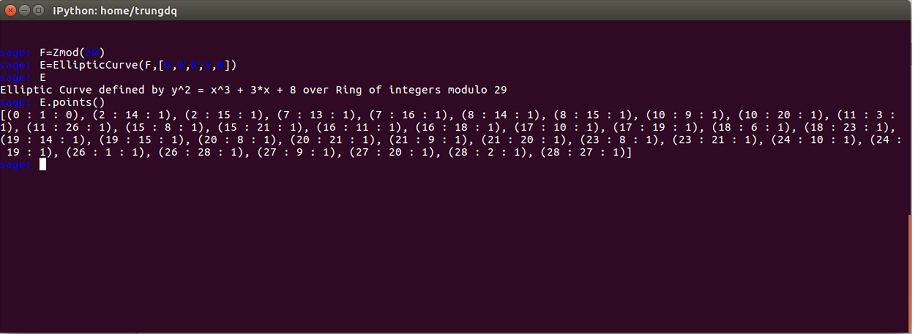
\includegraphics[width=1\linewidth]{../im16.png}
\caption{Các điểm trên elliptic với trường $\mathbb{F}_{29}$} \label{h16}
\end{figure}
\end{center}

Trong hình \ref{h16} tọa độ của mỗi điểm $(X, Y)$ có dạng $(x, Y, z)$ với $X = x/z$ (mod 29). Điểm $(0, 1, 0)$ chính là điểm $\mathcal{O}$. Ví dụ về cách viết này, điểm $(6, 9, 2)$ sẽ tương đương với điểm $(6 * 2^{-1ư} \ ( mod \ 29 ), 9) = (3, 9)$ \\

Hình \ref{h11}, bên trái là đồ thị đường cong elliptic $E \ y^2 = x^3 + 3x + 8$ trên trường số thực, bên phải là đồ thị các điểm thuộc đường cong elliptic $E$ trên trường hữu hạn $\mathbb{F}_{29}$. Các điểm ngoại trừ điểm $\mathcal{O}$ của $E$ trên trường $\mathbb{F}_{29}(E(\mathbb{F}_{29}))$.

\begin{figure}[h]
\begin{subfigure}{.5\textwidth}
  \centering
  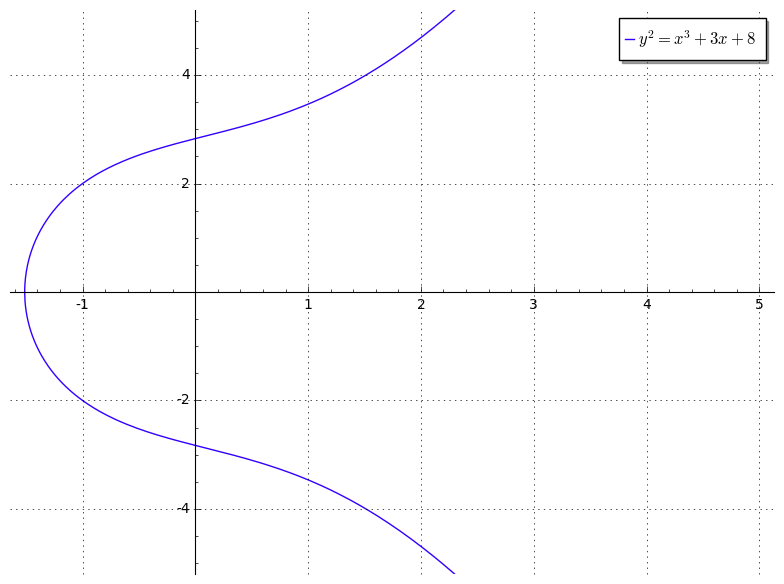
\includegraphics[width=1\linewidth]{../im11.png}
  \caption{1a elliptic trên trường số thực}
  \label{fig:sfig1}
\end{subfigure}%
\begin{subfigure}{.5\textwidth}
  \centering
  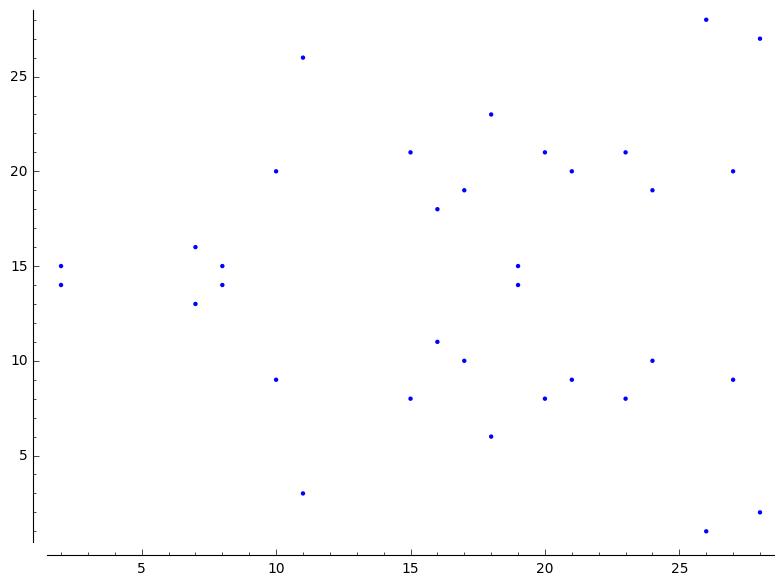
\includegraphics[width=1\linewidth]{../im12.png}
  \caption{1b elliptic trên trường hưu hạn $\mathbb{F}_{29}$}
  \label{fig:sfig2}
\end{subfigure}
\caption{Đường cong elliptic dạng $y^2 = x^3 + 3x + 8$} \label{h11}
\label{fig:fig}
\end{figure}
\begin{center}
\begin{tabular}{lllllll}
$(2, 14)$&  & $(2, 15)$&  & $(7, 13)$&  & $(7, 16)$ \\
$(8, 14)$&  & $(8, 15)$&  & $(10, 9)$&  & $(10, 20)$ \\ 
$(11, 3)$&  & $(11, 26)$&  & $(15, 8)$&  & $(15, 21)$ \\
$(16, 11)$&  & $(16, 18)$&  & $(17, 10)$&  & $(17, 19)$ \\
$(18, 6)$&  & $(18, 23)$&  & $(19, 14)$&  & $(19, 15)$ \\
$(20, 8)$&  & $(20, 21)$&  & $(21, 9)$&  & $(21, 20)$ \\
$(23, 8)$&  & $(23, 21)$&  & $(24, 10)$&  & $(24, 19)$ \\
$(26, 1)$&  & $(26, 28)$&  & $(27, 9)$&  & $(27, 20)$ \\
$(28, 2)$&  & $(28, 27)$ \\
\end{tabular}
\end{center}
Xét ví dụ thuật toán cộng (định lí \ref{dl2.2}) với hai điểm $P = (7, 13)$ và $Q = (8, 14)$ trong $E(\mathbb{F}_{29})$. Bước thứ e của thuật toán sẽ được tính đầu tiên
\begin{displaymath}
\lambda = \frac{y_2 - y_1}{x_2 - x_1} = \frac{14 - 13}{8 - 7} = \frac{1}{1} = 1,
\end{displaymath}
Ở đây các phép tính được thực hiện trên trường $\mathbb{F}_{29}$. Tiếp theo tính 
\begin{displaymath}
\vartheta = y_1 - \lambda x_1 = 13 - 1\cdot 7 = 6
\end{displaymath}
Cuối cùng phép cộng sẽ có kết quả
\begin{center}
\begin{tabular}{ll}
$x_3$ & = $\lambda^2 - x_1 - x_2 = 1 - 7 - 8 = -14 = 15$, \\
$y_3$ & = $-(\lambda x_3 + \vartheta) = -(1\cdot15 + 6) = -21 = 8$
\end{tabular}
\end{center}
Hay $P + Q = (7, 13) + (8, 14) = (15, 8)$ in  $E(\mathbb{F}_{29})$. Hình ảnh minh họa chạy bằng sagemath.
\begin{center}
\begin{figure}[H]
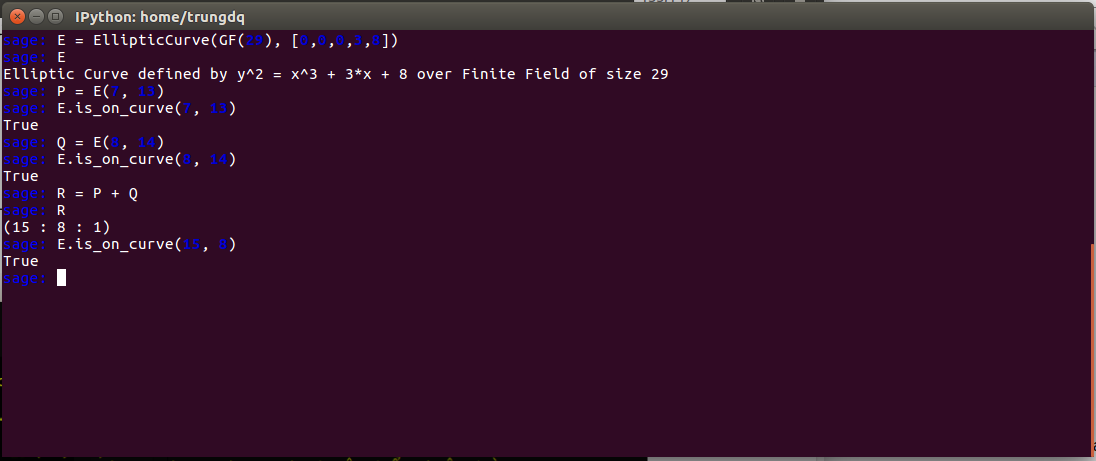
\includegraphics[width=0.9\linewidth]{../im17.png}
\caption{Ví dụ cộng hai điểm $P \neq Q$}
\end{figure}
\end{center}
\begin{center}
\begin{figure}[H]
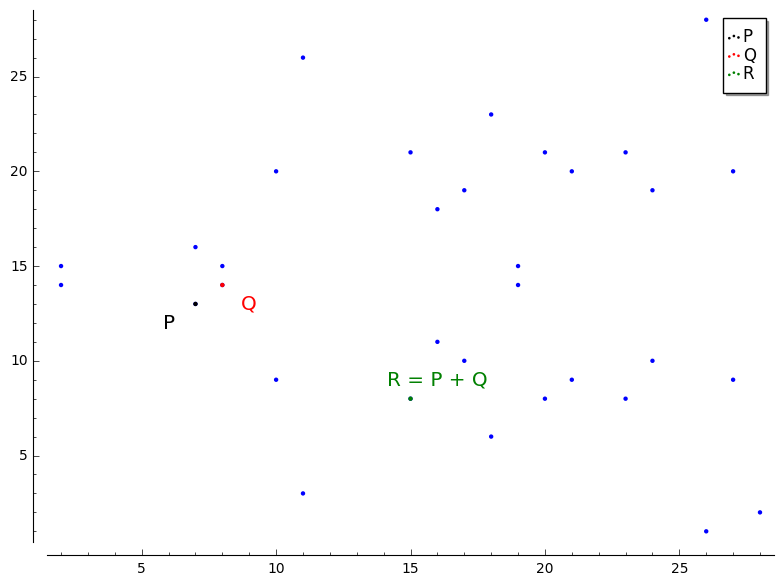
\includegraphics[width=0.8\linewidth]{../im13.png}
\caption{Biểu diễn $P + Q$ với ($P \neq Q$)}
\end{figure}
\end{center}
Tương tự ta có thể tính thuật toán cộng $P = (7, 13)$ với chính nó. Tính
\begin{center}
$\displaystyle \lambda = \frac{3x_1^2 + A}{2y_1} = \frac{3\cdot7^2 + 3}{2\cdot13} = \frac{150}{26} = \frac{5}{26} = 8$ \ và \ $\vartheta = y_1 - \lambda x_1 = 13 - 8\cdot7 = -68 = 15$
\end{center}
Ta có kết quả là 
\begin{center}
$x_3 = \lambda^2 - x_1 - x_2 = (8)^2 - 7 - 7 = 21$ và $y_3 = -(\lambda x_3 + v) = -(8\cdot21 + 15) = 20$,
\end{center}
vì vậy $P + P = (7, 13) + (7, 13) = (21,20)$ trong trường $E(\mathbb{F}_{29})$ là một điểm thuộc đường cong E (hình \ref{h18} và \ref{h14})
\begin{center}
\begin{figure}[H]
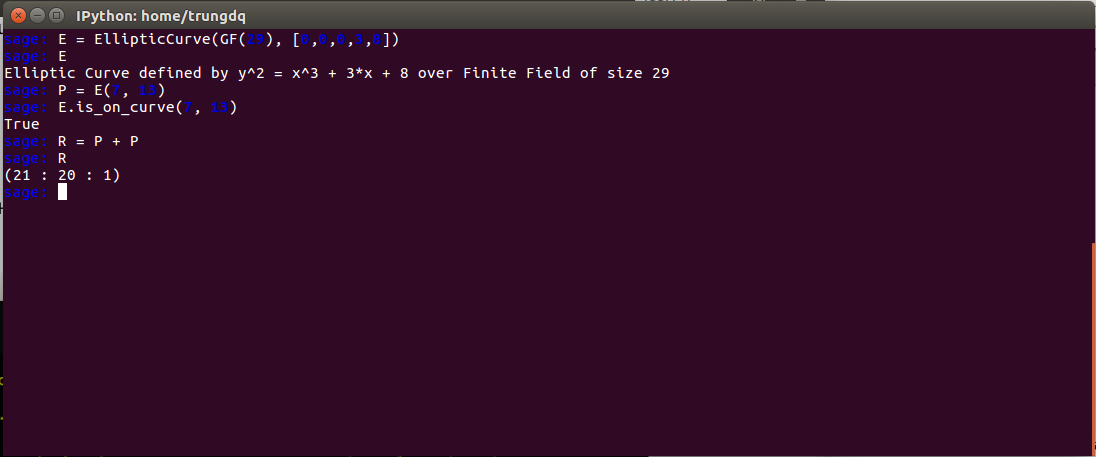
\includegraphics[width=0.9\linewidth]{../im18.png}
\caption{Ví dụ $2*P$ với ($P \neq \mathcal{O}$)} \label{h18}
\end{figure}
\end{center}

\begin{center}
\begin{figure}[H]
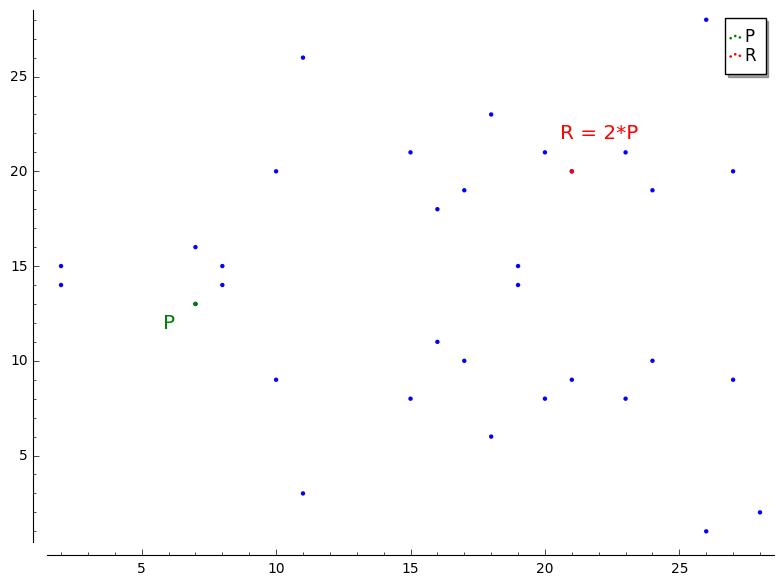
\includegraphics[width=0.8\linewidth]{../im14.png}
\caption{Biểu diễn $2*P$ với ($P \neq \mathcal{O}$)}
 \label{h14}
\end{figure}
\end{center}

Chọn điểm $P = (7, 13)$ suy ra điểm $-P = (7, -13 \ (\ mod \ 29 )= (7, 16))$ Ta có $P + (-P) = \mathcal{O}(hay \ \infty)$ (hình \ref{h19} và \ref{h19-1})

\begin{center}
\begin{figure}[H]
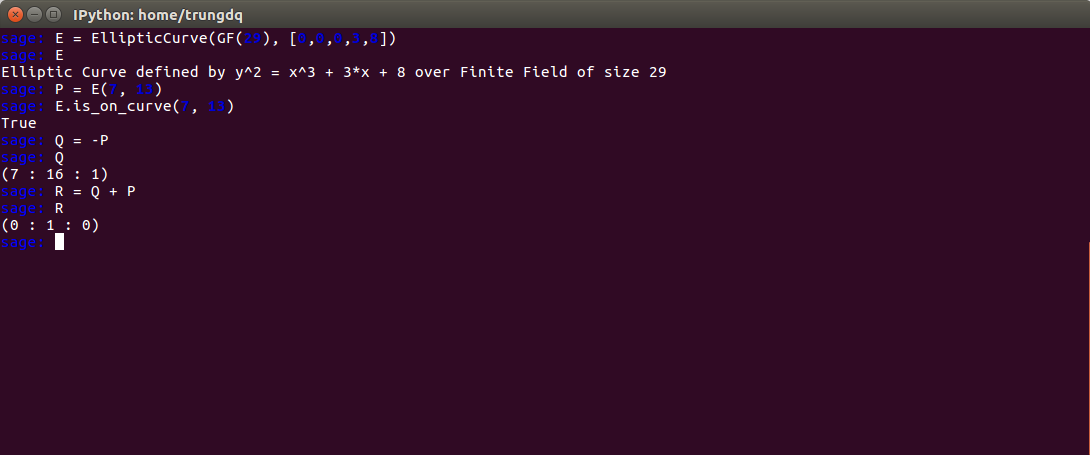
\includegraphics[width=0.9\linewidth]{../im19.png}
\caption{Ví dụ $2*P$ với ($P \neq \mathcal{O}$)} \label{h19}
\end{figure}
\end{center}

\begin{center}
\begin{figure}[H]
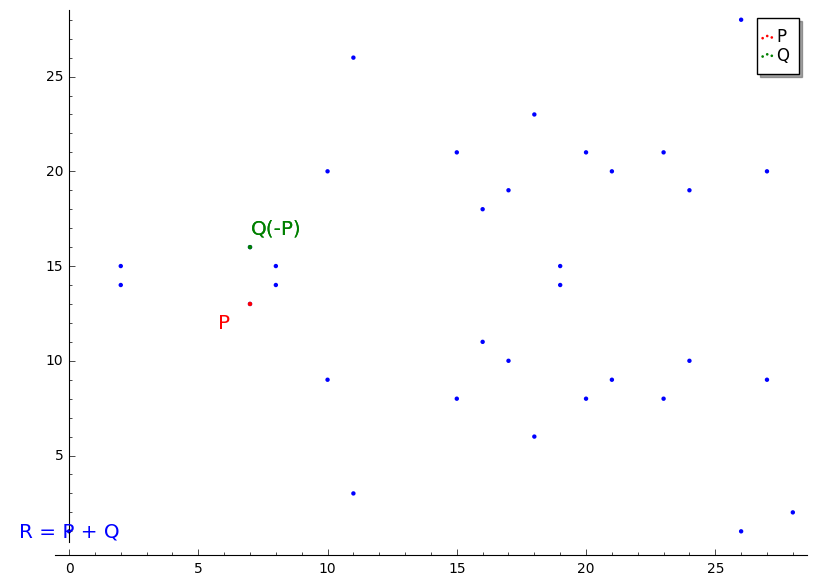
\includegraphics[width=0.8\linewidth]{../im15.png}
\caption{Biểu diễn $2*P$ với ($P \neq \mathcal{O}$)}  \label{h19-1}
\end{figure}
\end{center}
Trong vị dụ trên ta thấy điểm $P = (19, 15)$ là phần tử sinh \index{Phần tử sinh} của đường cong trên trường $\mathbb{F}_{29}$
\begin{center}
\begin{tabular}{lllllllll}
$P = (19, 15)$ & & $2P = (15, 8)$ & & $3P = (18, 23)$ & & $4P = (27, 20)$ \\
$5P = (21, 20)$ & & $6P = (17, 19)$ & & $7P = (26, 28)$ & & $8P = (20, 8)$ \\
$9P = (10, 9)$ & & $10P = (23, 21)$ & & $11P = (11, 26)$ & & $12P = (24, 10)$ \\
$13P = (16, 11)$ & & $14P = (28, 2)$ & & $15P = (7, 16)$ & & $16P = (2, 15)$ \\
$17P = (8, 14)$ & & $18P = (8, 15)$ & & $19P = (2, 14)$ & & $20P = (7, 13)$ \\
$21P = (28, 17)$ & & $22P = (16, 18)$ & & $23P = (24, 19)$ & & $24P = (11, 3)$ \\
$25P = (23, 8)$ & & $26P = (10, 20)$ & & $27P = (20, 21)$ & & $28P = (26, 1)$ \\
$29P = (17, 10)$ & & $30P = (21, 9)$ & & $31P = (27, 9)$ & & $32P = (18, 6)$ \\
$33P = (15, 21)$ & & $34P = (19, 14)$  \\
\end{tabular}
\end{center}
\subsection*{Thuật toán Double-and-Add}
\index{Thuật toán Double-and-Add}
Xuất phát từ việc khó phục hồi lại giá trị của n từ điểm $P$ và $Q = n\cdot P$ trong $E(\mathbb{F}_{p})$ đây là vấn đề khó của ECDLP. Tuy nhiên để sử dụng
\begin{displaymath}
\mathbb{Z} \rightarrow E(\mathbb{F}_p), \ \ \ n \mapsto nP,
\end{displaymath}
cho mật mã, chúng ta cần thực hiện phép tính $nP$ hiệu quả khi biết giá trị của $n$ và $P$. Nếu như $n$ lớn thì chúng ta chẳng muốn tính $nP$ bằng cách $P, 2P, 3P, 4P, \ldots .$
Các toán tử sử dụng trong tính toán đường cong elliptic được viết như phép cộng vì thế chúng ta sẽ gọi nó là "doubling-and-add". Ý tưởng cơ bản của thuật toán là chúng ta sẽ phân tích số n thành biểu diễn nhị phân
\begin{center}
$n = n_0 + n_1\cdot2 + n_2\cdot4 + n_3\cdot8 + \ldots + n_r\cdot2^r$ với $n_0, n_1, \ldots , n_r \in \{0, 1\}$.
\end{center}
Nếu chúng ta giả sử $n_r = 1$. Chúng ta có thể tính
\begin{displaymath}
Q_0 = P, \ \ Q_1 = 2Q_0, \ \ Q_2 = 2Q_1, \ldots , Q_r = 2Q_{r - 1}.
\end{displaymath}
Chú ý rằng $Q_i$, đơn giản chỉ là gấp hai lần $Q_{i-1}$ vì vậy 
\begin{displaymath}
Q_i = 2^iP.
\end{displaymath}
Các điểm là được biểu diễn như là phép với một số mũ cơ số 2, tính toán các điểm này yêu cầu r phép doubling. Cuối cùng chúng ta tính được $nP$ sử dụng r phép cộng
\begin{displaymath}
nP = n_0Q_0 + n_1Q_1 + n_2Q_2 + \ldots + n_rQ_r.
\end{displaymath}
Do đó tổng thời gian tính toán $nP$ tối đa là 2r phép toán trong $E(\mathbb{F}_p)$. Chú ý rằng $n \geq 2^r$, vì vậy không lớn hơn $2\log_2(n)$ phép toán để tính $nP$. Điều này tạo nên sự linh hoạt khi tính $nP$ thậm trí cả khi giá trị của n là lớn. Thuật toán tổng quát Double-and-Add.
\begin{algorithm}[H]
\caption{The double-and-add algorithm for elliptic curves}
\textbf{Input:} Điểm P nằm trường elliptic và số nguyên n >= 1
\begin{algorithmic}[1]
\State $Set \ Q = P \ and \  R = O$.
\State Loop while $n > 0$
\State \ \ \ \ If $n \equiv 1$ (mod 2), set $R = R + Q$.
\State \ \ \ \ $Q = 2Q$ and $n = \lfloor n/2 \rfloor$.
\State \ \ \ \ If $n > 0$, continue with loop at Step 2.
\State Return the point $R$, which equals $nP$.
\end{algorithmic}
\end{algorithm}
\section{Một số đường cong khác}
\subsection*{Montgomery curve}
\index{Montgomery Curve}
Trong toán học những đường cong Montgomery là một dạng của đường cong elliptic , khác với Weierstrass , được giới thiệu bởi Peter L. Montgomery vào năm 1987. Nó được sử dụng cho một số tính toán nhất định, và đặc biệt trong mật mã ứng dụng khác nhau.

Một đường cong Montgomery trên trường $\mathbb{K}$ được định nghĩa bởi phương trình 
\begin{displaymath}
M_{A,B}: By^2 = x^3 + Ax^2 + x
\end{displaymath}
với điều kiện $A, B \in \mathbb{K}$ và với $B(A^2 - 4) \neq 0$. Đường cong này được xem xét trên một trường hữu hạn $\mathbb{K}$($\mathbb{K} = \mathbb{F}_q$) với hai đặc điểm khác như $A \in \mathbb{K} \setminus \{-2, 2\}, B \in \mathbb{K} \setminus\{0\}$
\subsubsection{Luật cộng}
\index{Luật cộng}
Cho hai điểm $P_{1} = (x_{1}, y_{1}), P_{2}=(x_{2},y_{2})$ trên đường cong Montgomery $M_{A, B}$ trong hệ tọa độ affine, điểm $P_{3} = P_{1} + P_{2}$ biểu diễn hình học, điểm thứ ba là giao điểm giữa $M_{A, B}$ và đường thẳng đi qua $P_{1}$ và $P_{2}$. Có thể tìm tọa độ $(x_3, y_3)$ của $P_{3}$, theo cách sau:
\begin{itemize}
\item[1, ] Xem xét một đường thẳng $y = lx + m$ trong mặt phẳng affine và để nó đi qua $P_{1}$ và $P_{2}$ (áp đặt điều kiện), theo cách này, người ta có được $\displaystyle{l = \frac {y_{2} - y_{1}}{x_{2} - x_{1}}}$ và $\displaystyle{m = y_ {1} - \left({\frac {y_ {2} -y_ {1}} {x_ {2} -x_ {1}}} \right)x_{1}}$
\item[2, ] giao của đường thẳng với đường cong $M_{A, B}$, thay thế $y$ biến trong phương trình đường cong với $y = lx + m$ phương trình thu được:
\begin{displaymath}
x^3 + (A - Bl^2)x^2 + (1 - 2Blm)x - Bm^2 = 0.
\end{displaymath}
Như đã được quan sát trước đây, phương trình này có ba giải pháp tương ứng với tọa độ x của $P_{1}$,$P_{2}$ và $P_{3}$. Đặc biệt phương trình này có thể được viết lại thành:
\begin{displaymath}
(x - x_1)(x - x_2)(x - x_3) = 0
\end{displaymath}
\item[3, ] So sánh các hệ số của hai phương trình giống hệt nhau đã nêu ở trên, đặc biệt là các hệ số của các số hạng thứ hai, thu được:
\begin{displaymath}
-x_1 - x_2 - x_3 = A - Bl^2
\end{displaymath}
Vì thế, $x_3$ có thể được viết dưới dạng $x_{1}$, $y_{1}$, $x_{2}$, $y_{2}$, như:
\begin{displaymath}
x_3 = B\left(\frac{y_2 - y_1}{x_2 - x_1} \right)^2 - A - x_1 - x_2
\end{displaymath}
\item[4, ] Để tìm tọa độ y của điểm $P_{3}$, thay thế giá trị $x_{3}$ vào đường thẳng $y = lx + m$. Lưu ý rằng điều này sẽ không cho điểm $P_{3}$ trực tiếp. Thật vậy, với phương pháp này ta tìm thấy tọa độ của điểm $R$ sao cho $R + P_1 + P_2 = P_\infty$, nhưng  kết quả cần là tổng giữa $P_{1}$ và $P_{2}$, thì cần phải quan sát rằng: $R + P_1 + P_2 = P_\infty$ nếu và chỉ nếu $-R = P_1 + P_2$. Vì vậy, cho điểm $R$, nó là cần tìm $-R$, nhưng điều này có thể được thực hiện dễ dàng bằng cách thay đổi dấu y tọa độ của $R$. Nói cách khác, nó sẽ là cần thay đổi dấu của y bằng cách thay thế giá trị  $x_{3}$ trong phương trình đường thẳng.
Tóm lại tọa độ của điểm $P_3 = (x_3, y_3), P_3 = P_1 + P_2$ là:
\begin{displaymath}
x_3 = \frac{B(y_2-y_1)^2}{(x_2-x_1)^2}-A-x_1-x_2=\frac{B(x_2y_1-x_1y_2)^2}{x_1x_2(x_2-x_1)^2}
\end{displaymath}
\begin{displaymath}
y_3 = \frac{(2x_1+x_2+A)(y_2-y_1)}{x_2-x_1}-\frac{B(y_2-y_1)^3}{(x_2-x_1)^3}-y_1
\end{displaymath}
\end{itemize}
\subsubsection{Doubling}
\index{Doubling}
Cho một điểm $P_{1}$ trên đường cong Montgomery $M_{A, B}$, điểm $[2]P_1$ đại diện cho điểm hình học của điểm giao nhau thứ ba giữa đường cong và đường tiếp tuyến tại $P_{1}$; vì vậy, để tìm tọa độ của điểm $P_3 = 2P_1$, trong trường hợp này, đường thẳng $y  =  lx  +  m$ phải tiếp xúc với đường cong tại $P_{1}$, do đó, nếu $M_{A, B}: f(x, y) = 0$ với
\begin{displaymath}
f(x, y) = x^3 + Ax^2 + x - By^2
\end{displaymath}
giá trị của l biểu diễn hệ số góc của đường thẳng, cho bởi:
\begin{displaymath}
 l=-\left.\frac{\partial f}{\partial x}\right/\frac{\partial f}{\partial y}
\end{displaymath}
Vì vậy $\displaystyle l = \frac{3x_1^2 + 2Ax_1 + 1}{2By_1}$ và tọa độ điểm $P_3,P_3 = 2P_1$ là:
\begin{displaymath}
{\displaystyle {\begin{aligned}x_{3}&=Bl^{2}-A-x_{1}-x_{1}={\frac {B(3x_{1}^{2}+2Ax_{1}+1)^{2}}{(2By_{1})^{2}}}-A-x_{1}-x_{1}\\&={\frac {(x_{1}^{2}-1)^{2}}{4By_{1}^{2}}}={\frac {(x_{1}^{2}-1)^{2}}{4x_{1}(x_{1}^{2}+Ax_{1}+1)}}\\[8pt]y_{3}&=(2x_{1}+x_{1}+A)l-Bl^{3}-y_{1}\\&={\frac {(2x_{1}+x_{1}+A)(3{x_{1}}^{2}+2Ax_{1}+1)}{2By_{1}}}-{\frac {B(3{x_{1}}^{2}+2Ax_{1}+1)^{3}}{(2By_{1})^{3}}}-y_{1}.\end{aligned}}}
\end{displaymath}
\subsection*{Edwards curve}
\index{Edwards Curve}
Trong toán học , các đường cong Edwards là một họ các đường cong elip được Harold Edwards nghiên cứu năm 2007. Khái niệm về các đường cong elliptic trên các trường hữu hạn được sử dụng rộng rãi trong mã hóa đường cong elip. Các ứng dụng của các đường cong Edwards tới mật mã được Bernstein và Lange phát triển : chúng đã chỉ ra một số ưu điểm của dạng Edwards so với dạng Weierstrass.

Phương trình của một đường cong Edwards trên một trường $\mathbb{K} \neq 2$ là:
\begin{displaymath}
x^{2}+y^{2}=1+dx^{2}y^{2}
\end{displaymath}
cho một số vô hướng  $d \in \mathbb{K} \setminus \{0,1\}$. Ngoài ra dạng sau với các tham số c và d được gọi là đường cong Edwards:
\begin{displaymath}
x^2 + y^2 = c^2(1 + dx^2y^2)
\end{displaymath}
trong đó $c, d \in \mathbb{K}$ với $cd(1 - c^4\cdot d) \neq 0$ \\
Mỗi đường cong Edwards tương đương với đường cong elliptic ở dạng Weierstrass , và do đó thừa nhận luật nhóm đại số một khi ta chọn một điểm để phục vụ như là một phần tử trung lập. Nếu $\mathbb{K}$ là hữu hạn, thì một số lượng đáng kể tất cả các đường cong elliptic trên $\mathbb{K}$ có thể được viết dưới dạng đường cong Edwards. Thông thường các đường cong elip ở dạng Edwards được xác định có $c = 1$, không mất tính tổng quát. Trong các phần sau, giả sử rằng $c = 1$(xem thêm [11]).
\subsubsection{Luật cộng}
\index{Luật cộng}
Trên bất kỳ đường cong elliptic nào, có một điểm gọi là phần tử đơn vị. Đối với đường cong Edwards, lấy phần tử trung tính là điểm $(0, 1)$, tổng các điểm $(x_1,  y_1)$ và $(x_2 ,y_2)$ được đưa ra bởi công thức:
\begin{displaymath}
(x_1, y_1) + (x_2, y_2) = \left( \frac{x_1y_2 + x_2y_1}{1 + dx_1x_2y_1y_2}, \frac{y_1y_2 - x_1x_2}{1 - dx_1x_2y_1y_2} \right).
\end{displaymath}
Nghịch đảo của bất kì điểm nào $(x_1, y_1)$ là $(-x_1, y_1)$. Người ta kiểm tra rằng điểm $(0, -1)$ có cấp là 2, và điểm $(\pm 1, 0)$ có cấp là 4, Trong thưc tế, một đường cong Edward luôn luôn có một điểm có cấp là 4 với tọa độ trong trường $\mathbb{K}$.

Nếu d không phải là một bình phương trong $\mathbb{K}$ và $\displaystyle (x_{1}, y_{1}), (x_{2}, y_{2}) \in \{(x, y)|x^{2} + y^{2} = 1 + dx^{2}y^{2} \}$, không có điểm đặc biệt có mẫu số $1 +  dx_1x_2y_1y_2$ và $1 -  dx_1 x_2y_1y_2$ bằng 0. Do đó, luật cộng Edwards là hoàn tất khi $d$ không phải là một bình phương trong trường $\mathbb{K}$. Điều này có nghĩa là các công thức sẽ làm việc tốt và không có lỗi với các phép toán doubling, phần tử đơn vị, phần tử âm. Nói cách khác, nó được định nghĩa cho tất cả các cặp điểm đầu vào trên đường cong Edwards trên $\mathbb{K}$ và kết quả cho tổng của các điểm đầu vào.
Nếu $d$ là một bình phương $\mathbb{K}$ , thì phép toán tương tự có thể có các điểm đặc biệt, tức là có thể có cặp $(x_1, y_1)$ và $(x_2, y_2)$ trong đó 1$ +  dx_1x_2y_1y_2 = 0$ hoặc $1 -  dx_1x_2y_1y_2 = 0$.
Một trong những tính năng hấp dẫn của luật cộng của Edwards là nó được thống nhất mạnh mẽ, tức là nó cũng có thể được sử dụng để gấp đôi một điểm, đơn giản hóa việc bảo vệ chống lại tấn công bên kênh. Công thức cộng ở trên nhanh hơn các công thức thống nhất khác và có tính chất hoàn chỉnh mạnh.
\subsubsection{Doubling}
\index{Doubling}
Doubling có thể được thực hiện với chính xác công thức tương tự như cộng. Doubling đề cập đến trường hợp trong đó các đầu vào $(x_1, y_1)$ và $(x_2, y_2)$ được biết là bằng nhau. Vì $(x_1, y_1)$ nằm trên đường cong Edwards, ta có thể thay thế hệ số bằng $(x_1^2 + y_1^2  - 1)/x_1^2y_1^2$ như sau:
\begin{displaymath}
{\begin{aligned}2(x_{1},y_{1})&=(x_{1},y_{1})+(x_{1},y_{1})\\[6pt]2(x_{1},y_{1})&=\left({\frac  {2x_{1}y_{1}}{1+dx_{1}^{2}y_{1}^{2}}},{\frac  {y_{1}^{2}-x_{1}^{2}}{1-dx_{1}^{2}y_{1}^{2}}}\right)\\[6pt]&=\left({\frac  {2x_{1}y_{1}}{x_{1}^{2}+y_{1}^{2}}},{\frac  {y_{1}^{2}-x_{1}^{2}}{2-x_{1}^{2}-y_{1}^{2}}}\right)\end{aligned}}
\end{displaymath}
Điều này làm giảm mức độ mẫu số từ 4 đến 2, được phản ánh trong doubling. Luật cộng chung trong các tọa độ Edwards mất $10M + 1S + 1C + 1D + 7a$ và chi phí phép doubling là $3M + 4S + 3C + 6a$. Trong đó M là phép nhân trường, S là các phép bình phương trong trường , D là chi phí nhân với một tham số đường cong có thể lựa chọn và một trường bổ sung.
\subsection*{Twisted Edwards curve}
\index{Twisted Edwards Curve}
Trong hình học đại số , các đường cong Twisted Edwards là mô hình mặt phẳng của các đường cong elip , một sự tổng quát của các đường cong Edwards được giới thiệu bởi Bernstein , Birkner, Joye, Lange và Peters trong năm 2008. Bộ đường cong được đặt tên theo nhà toán học Harold M. Edwards . Đường cong Elliptic rất quan trọng trong mật mã khóa công khai và các đường cong Twist Edwards nằm ở trung tâm của một lược đồ chữ ký điện tử \index{Chữ ký điện tử} gọi là EdDSA mang lại hiệu năng cao trong khi tránh các vấn đề bảo mật xuất hiện trong các chương trình chữ ký số khác.

Như tên cho thấy, mỗi đường cong Twist Edwards là một xoắn của một đường cong Edwards. Đường cong Twist Edwards $E_{a, d}$ trên một trường $\displaystyle \mathbb{K}$ trong đó có $\displaystyle \mathrm{char}(\mathbb{K}) \neq 2$ là một đường cong mặt phẳng affine được xác định bởi phương trình:
\begin{displaymath}
E_{E_{a,d}}: ax^2 + y^2 = 1 + dx^2y^2
\end{displaymath}
Ở đâu $a, d$ là các phần tử khác 0 của $\displaystyle \mathbb{K}$. Đường cong Edwards là đường cong Twist Edwards với a = 1.
Mỗi đường cong Twist Edwards đều tương đương với đường cong elliptic ở dạng Montgomery và ngược lại.(xem [11])
\subsubsection{Luật cộng}
\index{Luật cộng}
Cho $\displaystyle \mathbb{K}$ là một trường có đặc điểm là khác 2. Để $\displaystyle (x_{1}, y_{1})$ và $\displaystyle (x_{2}, y_{2})$ là điểm trên đường cong Twist Edwards. Phương trình của đường cong Twist Edwards được viết như:
\begin{displaymath}
E_{E,a,d}: ax^2 + y^2 = 1 + dx^2y^2.
\end{displaymath}
Tổng của $(x_1, y_1)$ và $(x_2, y_2)$ trên $E_{E,a,d}$ là:
\begin{displaymath}
(x_{1}, y_{1}) + (x_{2}, y_{2}) = \left({\frac {x_{1}y_{2} + y_{1}x_{2}} { 1 + dx_{1}x_{2}y_{1}y_{2}}}, {\frac{y_{1}y_{2} - ax_{1}x_{2}} {1 - dx_{1}x_{2}y_{1}y_{2}}} \right)
\end{displaymath}
Phần tử đơn vị là $(0,1)$ và âm của điểm $(x_1, y_1)$ là $(-x_1, y_1)$. Công thức này cũng làm việc với doubling. Nếu a là một bình phương trong $\mathbb{K}$ và d không phải bình phương trong $\mathbb{K}$, công thức trên là hoàn tất. Điều này có nghĩa là chúng ta có thể công thức cho tất cả các cặp điểm mà không xảy ra ngoai lệ.
\subsubsection{Doubling}
\index{Doubling}
Doubling có thể được thực hiện với chính xác công thức tương tự như phép cộng. Doubling một điểm $(x_1 , y_1)$ trên đường cong $E_{E,a,d}$ là: $[2](x_1, y_1) = (x_3, y_3)$ ở đây
\begin{displaymath}
\begin{aligned}
x_{3} &= {\frac{x_{1}y_{1}+y_{1}x_{1}}{1+dx_{1}x_{1}y_{1}y_{1}}}={\frac {2x_{1}y_{1}}{ax_{1}^{2}+y_{1}^{2}}} \\[6pt]
y_{3} &= {\frac {y_{1}y_{1} - ax_{1}x_{1}}{1 - dx_{1}x_{1}y_{1}y_{1}}}={\frac{y_{1}^{2} - ax_{1}^{2}}{2 - ax_{1}^{2} - y_{1}^{2}}}.
\end{aligned}
\end{displaymath}
\section{Mật mã dựa trên đường cong Elliptic}
Chúng ta bắt đầu với ứng dụng đơn giản nhất, trao đổi khóa Diffie – Hellman, ít liên quan đến việc thay thế vấn đề logarit rời rạc cho trường $\mathbb{F}_p$ hữu hạn với bài toán logarit rời rạc cho đường cong elliptic $E(\mathbb{F}_p)$. Sau đó chúng ta sẽ mô tả các tương tự elliptic của hệ thống mã khóa công khai Elgamal và thuật toán chữ ký số (DSA).
\subsection*{Thông số miền (domain parameter)}
\index{Thông số miền}
Trong những phần trên ta đã xem xét những lý thuyết về đường cong elliptic. Để xác định một đường cong elliptic, người ta dựa trên những thông số miền, hay nói cách khác thông số miền đại diện cho một đường cong elliptic.

Có hai loại thông số miền được sử dụng đó là thông số miền cho đường cong elliptic trên trường hữu hạn $\mathbb{F}_p$ và trên trường hữu hạn $\mathbb{F}_{2^m}$. Nhưng ở đây chúng ta chỉ xem xét với trường $\mathbb{F}_p$ (tham khảo các thông số có sẵn ở [7]).

Các thông số miền của đường cong elliptic trên trường hữu hạn $\mathbb{F}_p$ là tập $T$:
\begin{displaymath}
T = (p, a, b, G, n, h)
\end{displaymath}

Trong đó số nguyên $p$ biểu thị trường hữu hạn $\mathbb{F}_p$. $a , b$ biểu thị hai phần tử của trường hữu hạn $\mathbb{F}_p$ thõa mãn công thức:
\begin{displaymath}
E: y^2 = x^3 + ax^2 + b \ (\ mod \ p)
\end{displaymath}

$G$ là điểm cơ sở $(x_G, y_G)$ thuộc $E(\mathbb{F}_p)$ hay còn gọi là phần tử sinh. $n$ là bậc của $G$ và số nguyên $h = \#E(\mathbb{F}_p)/n$.

Tập $T$ chỉ ra một đường cong elliptic với một phần tử sinh $G$.
\subsubsection{Sinh các thông số miền của đường cong elliptic trên trường $\mathbb{F}_p$}
Các thông số miền của đường cong elliptic được sinh ra theo các bước như sau:
\begin{itemize}
\item[] \textbf{Đầu vào:} Một số nguyên $t \in \{80, 112, 128, 192, 256\}$. Số nguyên $t$ này biểu thị mức độ bảo mật tính bằng bit của hệ các thông số miền được sinh ra. Có thể có thêm một phần tử hạt giống S.
\item[] \textbf{Đầu ra:} Các thông số miền của đường cong elliptic trên trường $\mathbb{F}_p$.
\begin{displaymath}
E: y^2 = x^3 + ax^2 + b \ (\ mod \ p)
\end{displaymath}
Như vậy thì việc tính logarithm rời rạc trên đường cong elliptic sẽ cần tới $2^t$ phép toán. Ngược lại, việc tính lũy thừa lại rất đơn giản
\item[] \textbf{Các bước sinh thông số miền:} Thông số miền được sinh ra theo các bước sau:
\begin{itemize}
\item[1. ] Chọn một số nguyên $p$ mà $\lceil log_2p \rceil = 2^t$ nếu $80 < t < 256$, $\lceil log_2p \rceil = 521$ nếu $t = 256$ và $log_2p = 192$ nếu $t = 80$
\item[2. ] Chọn hai số $a, b$ xác định đường cong elliptic $E(\mathbb{F}_p)$ theo công thức:
\begin{displaymath}
E: y^2 = x^3 + ax^2 + b \ (\ mod \ p)
\end{displaymath}
Chọn một điểm cơ sở $G = (x_G, y_G)$ trên đường cong elliptic $E(\mathbb{F}_p)$, một số nguyên $n$ là bậc của $G$. Số nguyên $h = \#E(\mathbb{F}_p)/n$. Tất cả thõa mãn các điều kiện sau:
\begin{itemize}
\item $47a^3 + 27b^2 \neq 0 (\ mod \ p)$
\item $\#E(\mathbb{F}_p) \neq p$ 
\item $p^B \neq 1$ với tất cả các giá trị $B$ nguyên $1 \leq B < 100$
\item $h \leq 2^{t/8}$
\item $n - 1$ và $n + 1$ nên có một phần tử lớn r (khi phân tích mỗi số thành thừa số nguyên tố) thõa mãn $\displaystyle log_n(r) > \frac{19}{20}$
\end{itemize}
\item[3. ] Xuất ra $T = (p, a, b, G, n, h)$
\end{itemize}
\end{itemize}
\subsection*{Trao đổi khóa với Elliptic Diffie-Hellman}
\index{Trao đổi khóa với Elliptic Diffie-Hellman}
Alice và Bob đồng ý sử dụng một đường cong elliptic đặc biệt $E(\mathbb{F}_p)$ và một điểm cụ thể $P \in E(\mathbb{F}_p)$. Alice chọn số nguyên $n_A$ bí mật và Bob chọn số nguyên $n_B$ bí mật. Họ tính toán các bội số liên quan
\begin{displaymath}
\overbrace{Q_A = n_AP}^{Alice} \ \ \ and \ \ \ \overbrace{Q_B = n_BP}^{Bob}
\end{displaymath}
và họ trao đổi các giá trị của $Q_A$ và $Q_B$. Sau đó Alice sử dụng hệ số bí mật của mình để tính toán $n_AQ_B$, và Bob tương tự tính toán $n_BQ_A$. Bây giờ họ có giá trị bí mật được chia sẻ
\begin{displaymath}
n_AQ_B = (n_An_B)P = n_BQ_A,
\end{displaymath}
mà họ có thể sử dụng như một chìa khóa để giao tiếp riêng tư thông qua một mật mã đối xứng. Tổng quát trao đổi khóa elliptic Diffie–Hellman
\begin{figure}[H]
\begin{center}
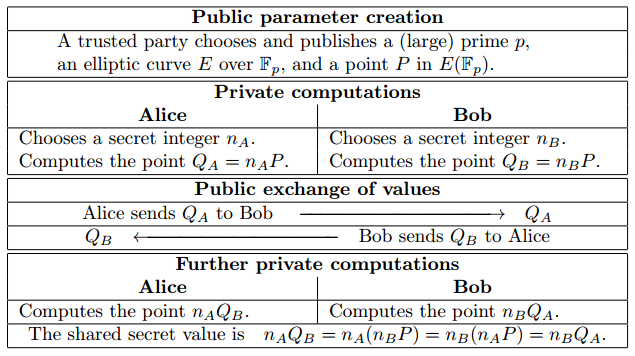
\includegraphics[scale=0.9]{../im7.png}
\caption{Trao đồi khóa Diffe-Hellman sử dụng đường cong elliptic}
\end{center}
\end{figure}
\subsection*{Hệ thống mã khóa công khai Elgamal}
\index{El-Gamal}
Alice và Bob đồng ý sử dụng một số nguyên tố $p$ cụ thể, đường cong elliptic $E$ và điểm $P \in E(\mathbb{F}_p)$. Alice chọn một số nhân $n_A$ bí mật và điểm $Q_A = n_AP$ làm khóa công khai của cô ấy. Nội dung của Bob là một điểm $M \in E(\mathbb{F}_p)$. Anh ta chọn một số nguyên k là yếu tố ngẫu nhiên của anh ấy và các tính toán
\begin{displaymath}
\ \ \ \ C_1 = kP \ \ \ \ and \ \ \ \ C_2 = M + kQ_A.
\end{displaymath}
Anh ấy sẽ gửi hai điểm $(C_1, C_2)$ đến Alice và Alice sẽ tính:
\begin{displaymath} 
C_2 - n_AC_1 = (M + kQ_A) - n_A(kP) = M + k(n_AP) - n_A(kP) = M
\end{displaymath}
để phục hồi bản rõ. Tổng quát hệ mã khóa công khai Elgamal \\
\begin{figure}[H]
\begin{center}
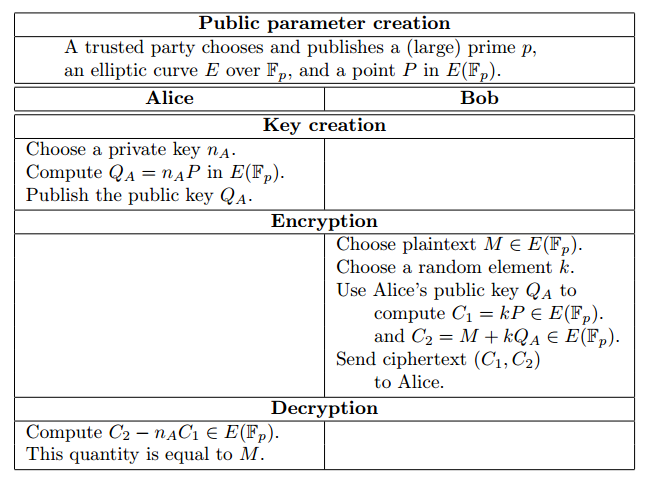
\includegraphics[scale=0.9]{../im5.png}
\caption{Tạo khóa, mã hóa, giải mã sử dụng Elliptic Elgamal}
\end{center}
\end{figure}
Trong thực tế, hệ mã khóa công khai Elgamal elliptic hoạt động tốt, nhưng có một số khó khăn thực tế
\begin{itemize}
\item[1, ] Không có cách rõ ràng để đính kèm các tin nhắn văn bản vào các điểm trong $E(\mathbb{F}_p)$
\item[2, ] Hệ thống mã hóa elgamal elliptic có hệ số mở rộng 4 đến 1, so với tỷ lệ mở rộng 2 đến 1 của Elgamal khi sử dụng $\mathbb{F}_p$.
\end{itemize}
Lý do elgamal elip có một mở rộng thông điệp 4 đến 1 nằm trong thực tế là bản rõ M là một điểm duy nhất trong $E(\mathbb{F}_p)$. Bản mã $(C_1, C_2)$ bao gồm bốn số modulo $p$, vì mỗi điểm trong $E(\mathbb{F}_p)$ có hai tọa độ. Các phương pháp khác nhau đã được đề xuất để giải quyết những vấn đề này. Khó khăn trong việc liên kết các bản rõ với các điểm có thể được phá vỡ bằng cách chọn M ngẫu nhiên và sử dụng nó làm mặt nạ cho bản rõ thô thực sự.
Với ví dụ Alice và Bob. Thật không may, vì Alice phải tính toán $C_2 - n_AC_1$ ,cô ấy cần các giá trị chính xác của cả hai tọa độ x và y của $C_1$ và $C_2$. Tuy nhiên, tọa độ x của một điểm xác định tọa độ y lên để thay đổi dấu, vì vậy Bob có thể gửi thêm một bit, ví dụ
\begin{displaymath}
\lambda = \left\{ \begin{array}{ll}
\displaystyle 0 & if \  0 \leq y \leq \frac{1}{2}p,\\
\\
\displaystyle 1 & if \ \frac{1}{2} < y < p
\end{array} \right.
\end{displaymath}
Theo cách này, Bob chỉ cần gửi các tọa độ x của $C_1$ và $C_2$, cộng thêm hai bit phụ. Ý tưởng này đôi khi được gọi là nén điểm.
\subsection*{Thuật toán chữ ký số với Elliptic}
\index{Thuật toán chữ ký số với Elliptic}
Thuật toán chũ ký số với Elliptic được mô tả sau đây:\\
\begin{figure}[H]
\begin{center}
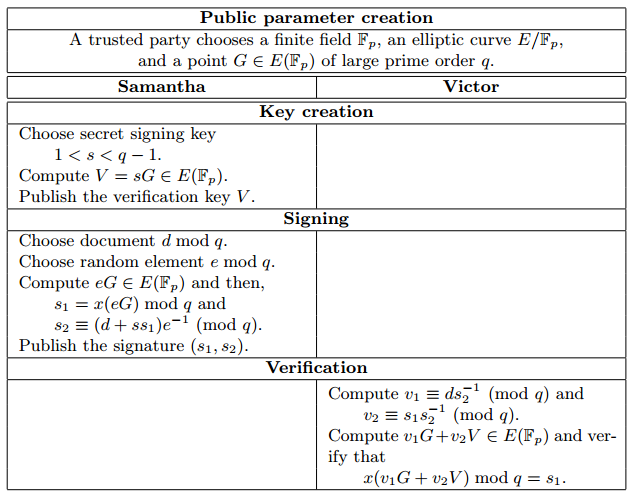
\includegraphics[scale=0.9]{../im6.png}
\caption{Chữ ký số ECDSA}
\end{center}
\end{figure}
tương tự như thuật toán chữ ký số đơn giản của DSA. ECDSA đang được sử dụng rộng rãi, đặc biệt là trong các tình huống mà kích thước chữ ký là quan trọng. \\

Để chứng minh rằng ECDSA hoạt động, tức là bước xác minh thành công trong việc xác minh chữ ký hợp lệ, chúng ta tính toán:
\begin{displaymath}
\begin{aligned}
v_1G + v_2V & = ds_2^{-1}G + s_1s_2^{-1}(sG) \\
            & = (d + ss_1)s_2^{-1}G \\
            & = (es_2)s_2^{-1}G \\
            & = eG \in E(\mathbb{F}_p).
\end{aligned}
\end{displaymath}
Do đó:
\begin{displaymath}
x(v_1G + v_2V) \mod \ q = x(eG)
\end{displaymath}
Chữ kí được chấp nhận là hợp lệ.
\section{Đường cong curve25519}
\index{Đường cong curve25519}
\subsection{Định nghĩa}

\begin{center}
\begin{figure}[H]
\centering
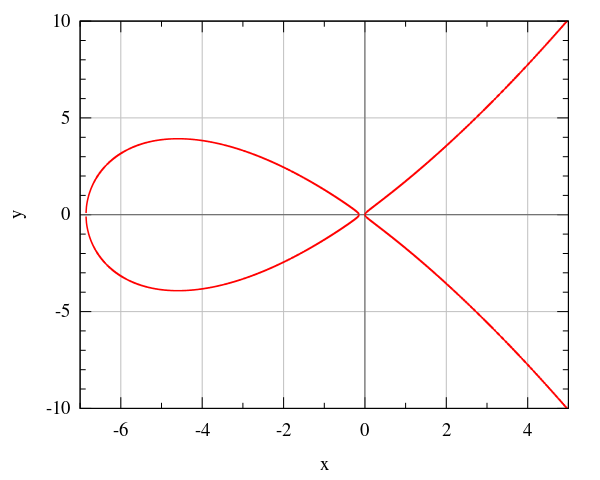
\includegraphics[width=0.7\linewidth]{../mo.png}
\caption{ Đường cong Montgomery (nguồn: wikipedia.org)}
\end{figure}
\end{center}

Curve25519 là một đường cong elliptic trên trường hữu hạn $\mathbb{F}_p$ với $p = 2^{255} - 19$, được Daniel J. Brenstein giới thiệu trong bài báo "Curve25519: new Diffie-Hellman speed records". Curve25519 có rất nhiều ưu điểm vượt trội so với các đường cong khác như tốc độ tính toán,
khả năng bảo mật cao. Công thức của đường cong Curve25519:
\begin{displaymath}
By^2 = x^3 + Ax^2 + x
\end{displaymath}
Công thức này đã được đề cập ở phần trước. Nhờ sử dụng công thức của Montgomery, đường cong Curve25519 có được nhiều ưu điểm nổi bật mà các đường cong khác không sử dụng công thức của Montgomery không có được. Cụ
thể hơn, nhờ sử dụng công thức cộng và nhân đôi của Montgomery, curve25519 có thể chống lại timing-attack \index{Timing-attack}.
\begin{itemize}
\item[] \textbf{Ưu điểm đường cong Curve25519}
\begin{itemize}
\item[1. ] \textbf{Tốc độ tính toán cao}: Curve25519 cho tốc độ tính toán cao hơn so với các đường cong khác mà vẫn giữ được tính bảo mật cao.
\item[2. ] \textbf{Có khả năng chống lại timing-attack}: Nhờ sử dụng công thức cộng và bình phương Montgomery, Curve25519 có khả năng chống lại timing-attack mà vẫn đảm bảo được tốc độ tính toán cao
\item[3. ] \textbf{Khóa bí mật và khóa công khai ngắn}: Curve25519 sử dụng khóa bí mật có độ dài chỉ 32-byte(256-bit). Đây là độ dài tiêu chuẩn nhưng vẫn cho độ bảo mật cao. Khóa công khai của Curve25519 cũng chỉ có độ dài 32-byte.
\end{itemize}
\end{itemize}
\subsection{Trao đổi khóa với đương cong Curve25519}
Đường cong Curve25519 sử dụng một khóa bí mật và một khóa công khai, cả hai đều có độ dài 32-byte (256-bit). Với những phương pháp tấn công đã biết thì với độ dài khóa như vậy, Curve25519 có mức độ bảo mật tương đương một hệ mã khóa đối xứng 128-bit. Có nghĩa là để tấn công hệ mã này, người ta sẽ phải vét cạn một không gian khóa có độ lớn $2^{128}$.

Hàm Curve25519(a, b) có a, b là các phần tử của trường hữu hạn $\mathbb{F}_p$ với $p = 2^{255} - 19$ như đã nói ở trên. Hàm này cho kết quả là một số $n \in \mathbb{F}_p$. Hay nói cách khác:
\begin{displaymath}
Curve25519(a, b): \mathbb{F}_{p^2} \rightarrow \mathbb{F}_p
\end{displaymath}
Với hàm Curve25519(a, b) như thế, Alice và Bob muốn thống nhất với nhau một khóa bí mật $k$, họ làm như sau với đường cong:
\begin{displaymath}
y^2 = x^3 + 486662x^2 + x
\end{displaymath}
\begin{itemize}
\item[1. ] Alice tạo khóa bí mật $a \in 2^{254} + 8\{0, 1, 2, \ldots, 2^{251} - 1\}$. Alice tính khóa công khai là $A = Curve25519(a, 9)$.
\item[2. ] Bob tạo khóa bí mật $b \in 2^{254} + 8\{0, 1, 2, ..., 2^{251} - 1\}$. Bob tính khóa công khai là $B = Curve25519(b, 9)$.
\item[3. ] Alice tính $S: S = Curve25519(a, B)$.
\item[4. ] Bob tính $S: S = Curve25519(b, A)$.
\end{itemize}
Từ giá trị $S$ tính được, Alice và Bob sẽ sử dụng hàm băm để có giá trị khóa bí mật $s$ cần thống nhất $s = Hash(S)$.
\begin{center}
\begin{figure}[H]
\centering
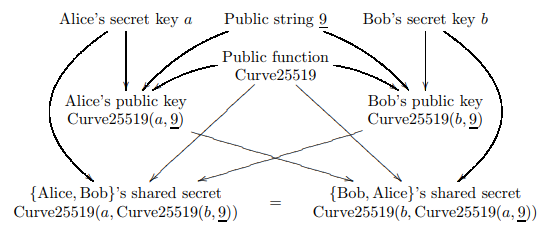
\includegraphics[width=0.85\linewidth]{../im23.png}
\caption{Sơ đồ trao đổi khóa Diffe-Hellman Elliptic Curve}
\end{figure}
\end{center}
\subsubsection{Hàm Curve25519}
\index{Hàm Curve25519}
Trong phần này chúng ta sẽ tìm hiểu cách chọn khóa bí mật $n$ và tính $Curves25519(n, 9)$ ở phần trước đã mô tả.
\begin{theorem} \label{dl4.1}
Chọn p là một số nguyên tố, $p \geq 5$. Chọn A là một số nguyên thõa mãn $A^2 - 4$ không phải là bình phương của một số nào đó theo modulo $p$. E là đường cong elliptic $y^2 = x^3 + Ax^2 + x$ trên trường hữu hạn $\mathbb{F}_p$. Định nghĩa hàm $X_0 : E(\mathbb{F}_{p^2} ) \rightarrow  \mathbb{F}_{p^2}$ như sau: $X_0(\infty) = 0$; $X_0(x, y) = x$. Với $n$ là một số nguyên, $q$ là một phần tử của $\mathbb{F}_p$. Thì sẽ tồn tại một phần tử $s$ đặc biệt $s \in \mathbb{F}_p$ sao cho $X_0(nQ) = s$ với tất cả các điểm $Q \in E(\mathbb{F}_{p^2} )$ thõa mãn $X_0(Q) = q$ (theo [?])
\end{theorem}

Theo định lý trên, lấy $p = 2^{255} - 19$, từ $p$ ta có trường hữu hạn $\mathbb{F}_{2^{255}-19}$. Chọn $A = 486662,A^2 - 4$ không phải là bình phương của bất kì số nào trên trường $\mathbb{F}_p$. $E$ là đường cong elliptic $y^2 = x^3 + 486662x^2 + x$ trên trường hữu hạn $\mathbb{F}_p$. Định nghĩa hàm $X_0 : E(\mathbb{F}_{p^2} ) \rightarrow \mathbb{F}_{p^2}$ như sau: $X_0(\infty) = 0; X_0(x, y) = x$. Với $n \in 2^{254} + 8\{0, 1, 2, \ldots, 2^{251} - 1\}$ và $q \in \mathbb{F}_p$, hàm Curve25519 sẽ cho kết quả là giá trị $s$.

Từ định lý trên giá trị $q = 9$ là hoành độ của điểm $Q \in E(\mathbb{F}_p)$. Điểm $Q$ này chính là điểm cơ sở của đường cong $E : y^2 = x^3 + 486662x^2 + x$ trên trường $\mathbb{F}_p$. Hay nói cách khác điểm $Q$ ở đây với hoành độ $x_Q = 9$ cũng là một phần tử sinh. Bởi vậy, để tính khóa công khai của Alice ta dùng hàm $Curve25519(a, 9)$.

Mặt khác $n \in 2^{254} + 8\{0, 1, 2, \ldots, 2^{251} - 1\}$ để đảm bảo cho $n_Q$ với $Q$ có hoành độ $x_Q = 9$ khác $\infty$ để $X_0(n_Q)$ , $\infty$ hay $Curve25519(n, 9) \neq 0$.

\subsubsection{Công thức cộng và nhân đôi Montgomery}
Đường cong elliptic như đã giới thiệu trong chương 3 sử dụng công thức cộng và nhân trên cả hai tọa độ $x$ và $y$. Kết quả của phép cộng và phép nhân hai điểm là một điểm thứ ba. Tuy nhiên với Curve25519, Daniel J. Bernstein có cái hay là thức cộng và nhân đôi Montgomery và tọa độ $y$ không tham gia vào các phép tính cộng và nhân. Thay vào đó, với điểm $Q$ có tọa độ
$(x_Q, y_Q)$ thì $x_Q$ sẽ được viết dưới dạng phân số $x/z$. Các phép toán cộng và bình phương sẽ được thực hiện trên $x$ và $z$ thay vì $x$ và $y$. Dĩ nhiên với cách viết như vậy ta sẽ không thể nào phân biệt được hai điểm $Q$ và $-Q$.
\begin{theorem}
Gọi tọa độ điểm $P$ là $(xP, zP)$, tọa độ điểm $Q$ là $(xQ, zQ)$, tọa độ điểm $P - Q$ là $(x_{P-Q}, z_{P-Q})$, tọa độ điểm $P + Q$ là $(x_{P+Q}, z_{P+Q})$, tọa độ của $2P$ là $(x_{2P}, z_{2P})$, tất cả các tọa độ trên đều khác với tọa độ của điểm $\mathcal{O}$.

Chọn $p$ là một số nguyên tố, $p \geq 54$. Chọn $A$ là một số nguyên thõa mãn $A^2 - 4$ không phải là bình phương của một số nào đó theo modulo $p$. $E$ là đường cong elliptic $y^2 = x^3 + Ax^2 + x$ trên trường hữu hạn $\mathbb{F}_p$. Định nghĩa hàm $X : E(\mathbb{F}_{p^2}) \rightarrow \mathbb{F}_{p^2}$ như sau: $X(\infty) = 0; X(x, y) = x$. Với các tọa độ các điểm được xác định như trên ta có [4]:
\end{theorem} 
\begin{itemize}
\item[] Phép cộng $P + Q (P \neq Q)$:
\begin{displaymath}
\begin{aligned}
x_{P+Q} & = 4(x_P x_Q - z_Pz_Q)^2z_{P-Q} & = ((x_P - z_P)(x_Q + z_Q) + (x_P + z_P)(x_Q - z_Q))^2z_{P-Q} \\
z_{P+Q} & = 4(x_Pz_Q - z_Px_Q)^2x_{P-Q} & = ((x_P - z_P)(x_Q + z_Q) - (x_P + z_P)(x_Q - z_Q))^2x_{P-Q}
\end{aligned}
\end{displaymath}
\item[] Phép double $2P$:
\begin{displaymath}
\begin{aligned}
x_{2P} & = (x^2_P - z^2_P)^2  = (x_P - z_P)^2(x_P + z_P)^2 \\
z_{2P} & = 4x_Pz_P(x^2_P + Ax_Pz_P + z^2_P) \\ & = ((x_P + z_P)^2 - (x_P - z_P)^2)\left((x_P + z_P)^2 + \frac{A - 2}{4}((x_P + z_P)^2 - (x_P - z_P)^2) \right)
\end{aligned}
\end{displaymath}
\end{itemize}

Theo như định lý trên, ta có thể tính được tọa độ của điểm $P + Q$ dựa trên tọa độ của ba điểm $P, Q$ và $P-Q$, tính được tọa độ của điểm $2P$ dựa trên tọa độ điểm $P$.

Tọa độ điểm $P+Q$ có thể tính được dựa vào tọa độ $P, Q$ và tọa độ của điểm $P-Q$ (tức tọa độ của điểm $((x_P, y_P) + (x_Q, -y_Q)))$ điều này có vẻ như mâu thuẫn với định lý \ref{dl4.1}, tuy nhiên trong định lý \ref{dl4.1} không có nhắc đến việc cộng hai điểm $P$ và $Q$ có tọa độ bất kì nên việc công thức cộng Montgomery có liên quan đến tọa độ $y$ là không vô lý.
\chapter{Chứng thư số ẩn dựa trên đường cong Elliptic}
Trong chương này xác định sơ đồ chứng thư số ẩn của Elliptic Curve Qu-Vanstone \index{Elliptic Curve Qu-Vanstone}(ECQV \index{ECQV}). Sơ đồ chứng thư số \index{Chứng thư số}ẩn ECQV được xem như là một lược đồ chứng thư với mục đích chung cho các ứng dụng trong các hệ thống máy tính và truyền thông. Nó đặc biệt thích hợp cho các môi trường ứng dụng nơi có các tài nguyên như băng thông, sức mạnh tính toán và lưu trữ bị hạn chế. ECQV cung cấp giải pháp thay thế hiệu quả hơn cho chứng chỉ truyền thống.

Mục đích của chương này là để xem xét việc triển khai sơ đồ chứng thư số ẩn 
\section{Hàm băm và Hàm băm một số nguyên modul n}
\subsection*{Hàm băm}
\index{Hàm băm}
Hàm băm được sử dụng trong lược đồ ECQV để tính toán thông điệp của chứng chỉ được tạo hoặc xác minh. Hàm băm cũng được sử dụng trong việc tạo và xác thực tham số miền elliptic ngẫu nhiên một cách chính xác, và cũng có thể được sử dụng trong các quá trình tạo số ngẫu nhiên.

Mức độ bảo mật kết hợp với hàm băm phụ thuộc vào ứng dụng của nó. Trường hợp tránh xung đột là cần thiết, mức độ bảo mật tối đa bằng một nửa độ dài đầu ra (tính theo bit) của hàm băm. Trường hợp tránh xung đột là không cần thiết, mức độ bảo mật tối đa là độ dài đầu ra (tính theo bit) của hàm băm. Khả năng tránh xung đột nói chung là cần thiết để tính toán thông điệp cho chữ ký số.

Hàm băm được sử dụng bởi sơ đồ ECQV sẽ được chấp nhận hàm băm, như được chấp thuận trong mục đăng ký X9 00003, tiêu chuẩn băm an toàn (SHS). Mức độ bảo mật của hàm băm được phê duyệt được coi là tối đa một nửa độ dài đầu ra của nó cho các mục đích của tiêu chuẩn này. Danh sách một số hàm hăm tiêu chuẩn SHA-1, SHA-2, MD5, \ldots.

Hàm băm được sử dụng để tính toán chứng thư ẩn sẽ là hàm băm có mức bảo mật ít nhất là mức bảo mật của việc triển khai ECQV. Hàm băm được sử dụng cho các xác định tham số  elliptic sẽ là hàm băm có mức bảo mật là mức độ bảo mật của việc triển khai sơ đồ ECQV (ngoại trừ các xác định tham số elliptic ngẫu nhiên trong [7] được tạo bằng cách sử dụng SHA-1).
\subsection*{Hàm băm một số nguyên modul n}
\index{Hàm băm một số nguyên modul n}
Trong nhiều bước của \index{ECQV}, một chuỗi octet(mỗi một ký tự trong xâu được biểu diễn bởi 8 bits) chiều dài tùy ý được băm bằng hàm băm mật mã $H$, và sau đó được chuyển đổi thành một số nguyên modulo $n$. Phần này chỉ định hàm kết quả, ký hiệu $H_n: \{0, 1,\ldots , 255\}^{*} \rightarrow [0,\ldots , n - 1]$, ánh xạ các chuỗi octet có độ dài tùy ý đến các số nguyên modulo n.
\begin{itemize}
\item[] \textbf{Input}
\begin{itemize}
\item[1. ] Một chuỗi octet có chiều dài tùy ý $S$.
\item[2. ] Hàm băm $H$ băm chuỗi octet chiều dài tùy ý thành các chuỗi bit dài của hashlen.
\item[3. ] Số nguyên $n$.
\end{itemize}
\item[] \textbf{Action}
\begin{itemize}
\item[1. ] Tính toán $h = H(S)$, một chuỗi bit dài hashlen bits.
\item[2. ] Lấy một số nguyên $e$ từ $h$ như sau:
\begin{itemize}
\item[2.1 ] Đặt E bằng $\lfloor log_2{n} \rfloor$ bits trái nhất của h.
\item[2.2 ] convert xâu bit $E$ thành xâu octect $E'$, sử dụng  Bit-String-to-Octet-String trong [6].
\item[2.3 ] convert xâu octect $E'$ thành số nguyên $e$ sử dụng Octet-String-to-Integer trong [6].
\end{itemize}
\end{itemize}
\item[] \textbf{Output} Số nguyên e, nằm trong khoảng $[0,\ldots , n - 1]$.
\end{itemize}
Lưu ý rằng nếu miền $H$ bị giới hạn ở kích thước tối đa thì miền $H_n$ bị hạn chế theo cùng một cách. 
\section{Sơ đồ chứng thư số thực ECQV}
\subsection{Tổng quan}
Sơ đồ chứng chỉ số ẩn được sử dụng bởi ba thực thể - Tổ chức phát hành chứng chỉ CA, người yêu cầu chứng chỉ U và bộ xử lý chứng chỉ V. Người yêu cầu U sẽ nhận được chứng chỉ số ẩn từ CA, xác nhận danh tính của U và cho phép V lấy khóa công khai của U. 
\begin{figure}[h]\label{h3.1}
\begin{center}
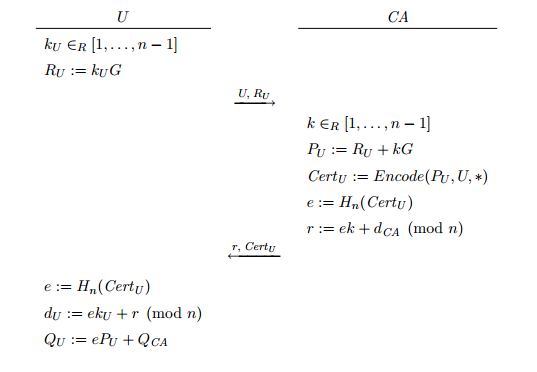
\includegraphics[scale=0.9]{../im8.png}
\caption{Sơ đồ chứng thư ẩn ECQV}
\end{center}
\end{figure}

Sơ đồ chứng thư số ẩn bao gồm sáu phần. Những phần này sẽ được sẽ được mô tả chi tiết.\\
\textbf{ECQV\_Setup}: Trong bước này, CA thiết lập các tham số đường cong elliptic, hàm băm, định dạng mã hóa chứng chỉ và tất cả các bên đã chọn một trình tạo số ngẫu nhiên. CA tạo ra một cặp khóa. Tất cả các bên phải nhận được bản sao xác thực các thông số và khóa công khai của CA. \\[6pt]
\textbf{Cert\_Request}: Người yêu cầu U phải tạo một yêu cầu cho một chứng chỉ, được gửi đến CA. Thành phần mật mã của yêu cầu là khóa công khai, được tạo ra bằng cách sử dụng cùng thủ tục như CA sử dụng trong khi thiết lập ECQV. \\ [6pt]
\textbf{Cert\_Generate}: Khi nhận được yêu cầu chứng chỉ từ U, CA xác nhận danh tính của U và tạo chứng chỉ số ẩn. CA gửi phản hồi cho U. \\ [6pt]
\textbf{Cert\_PK\_Extraction}: Với chứng chỉ số ẩn cho U người dùng, thông số và khóa công khai của CA, thuật toán trích xuất khóa công khai tính toán khóa công khai của U. \\ [6pt]
\textbf{Cert\_Reception}: Sau khi nhận được phản hồi cho yêu cầu chứng chỉ của mình, U đảm bảo tính hợp lệ của cặp khóa được chứng nhận ngầm

Cấp chứng thư là quy trình gồm hai bước, trong đó bước đầu tiên nhận được yêu cầu cấp chứng thư từ U và bước thứ hai là tạo phản hồi, chứa chứng thư. Hình \ref{h3.1} đã mô tả giao thức (thông tin).

Một số khác biệt giữa ECQV và chứng chỉ truyền thống liên quan đến việc ràng buộc giữa danh tính của người dùng và khóa công khai

\subsection{Điều kiện tiên quyết: Cài đặt ECQV}
Tất cả các bên (CA nhà phát hành chứng thư, chủ sở hữu chứng thư U và bộ xử lý chứng thư V) sẽ phải thiết lập các điều kiện tiên quyết sau để sử dụng ECQV.
\begin{itemize}
\item[1, ] CA đã thiết lập một tập hợp các tham số EC để sử dụng với ECQV bao gồm $q, a, b, G, n$ và $h$. Các tham số phải được tạo bằng phương thức được chấp nhận chúng phải được đảm bảo tính hợp lệ trên EC và cung cấp mức độ bảo mật mong muốn(có thể tham khảo các phương thức tạo tham số hoặc các tham số sẵn có ở [6, §3.1] và [7]).
\item[2, ] CA đã chọn một hàm băm được chấp nhận với mức độ bảo mật mong muốn để sử dụng trong quy trình tạo chứng thư ECQV. Giả sử $H$ là hàm băm đã chọn và hashlen là độ dài của đầu ra hàm $H$. Như trong phần trước đã mô tả convert đâu ra của $H$ là một số nguyên dương n.
\item[3, ] CA và U chọn và khởi một số ngẫu nhiên đảm bảo được mức độ bảo mật mong muốn. Số ngẫu nhiên này được sử dụng để tạo khóa private trong quá trình yêu cầu chứng thư và quá trình tạo chứng thư.
\item[4, ] CA tạo được cặp khóa trên EC $(d_{CA}, Q_{CA})$ liên quan với các tham số EC được thiết lập từ ban đầu để sử dụng trong quá trình tạo chứng thư. Cặp khóa sẽ được tạo ra bằng cách sử dụng điểm  sinh và số ngẫu nhiên tạo ở mục 3(xem ở [6, §3.2.1]). CA sẽ đảm bảo tính hợp lệ của cặp khóa và sự đảm bảo của quyền sở hữu của khóa riêng (xem [6]).
\item[5, ] Chủ sở hữu $U$ của chứng thư cùng với bộ xử lý $V$ sẽ thu được tham số đường cong, hàm băm và khóa công khai của CA là $Q_{CA}$. U và V sẽ có một số đảm bảo sau:
\begin{itemize}
\item[5.1, ] Tính hợp lệ các tham số đường cong EC.
\item[5.2, ] Tính hợp lệ khóa công khai của CA, $Q_{CA}$
\item[5.3, ] Sở hữu khóa riêng, $d_{CA}$ của CA
\end{itemize}
\end{itemize}
\subsubsection{Mã hóa chứng thư} \label{subsec:3.5.2.1}
Mã hóa chứng chứng thư mô tả cách thông tin được thêm vào trong chứng thư phải được mã hóa dưới dạng chuỗi octet. Nó cũng chỉ định thông tin nào phải được thêm vào và thông tin nào là tùy chọn và mọi ràng buộc hoặc mối quan hệ giữa các phần của thông tin chứng thư.

Có ba kiểu mã hóa chứng thư chính(tham khỏa mô tả chi tiết xem ở [8])
\begin{itemize}
\item[•] \textbf{Fixed-length Fields}: là một mã hóa đơn giản, tối giản giúp đặt hiệu quả băng thông lên trước tất cả các mối quan tâm khác. Chứng chỉ bao gồm danh sách các trường, mỗi trường có độ dài cố định và định dạng được chia sẻ giữa tất cả các bên. Tiêu chuẩn này chỉ yêu cầu dữ liệu tái tạo khóa công khai PU là một trong các trường, để phần còn lại của định dạng mở cho người triển khai.
\item[•] \textbf{Minimal ASN.1 Encoding Scheme}: cũng được thiết kế để có hiệu quả băng thông. Đặc tả ASN.1 bao gồm các trường bắt buộc cơ bản và cho phép các phần mở rộng. Các trường cơ bản được đề xuất trong mã hóa này có độ dài cố định và do đó cũng có thể được sử dụng với định dạng độ dài cố định đơn giản hơn.
\item[•] \textbf{X.509-Compliant ASN.1 Encoding}: được thiết kế để bao gồm thông tin đầy đủ để cho phép chứng chỉ ECQV này được mã hóa lại dưới dạng chứng chỉ X.509 chuẩn.
\end{itemize}
\subsection{Yêu cầu chứng thư: Cert\_Request}
Người yêu cầu chứng chỉ U, sẽ sử dụng quy trình dưới đây để tạo yêu cầu chứng chỉ.
\begin{itemize}
\item[] \textbf{Input}
\begin{itemize}
\item[1. ] Các tham số đường cong EC được thiết lập bởi CA.
\item[2. ] Xâu biểu diễn định danh của U.
\end{itemize}
\item[] \textbf{Actions}
\begin{itemize}
\item[1. ] Khởi tạo cặp khóa $(k_u, R_u)$  trên EC liên quan tới các tham số được thiết lập với đường cong(tham khảo cách tạo cặp khóa ở [6, §3.2.1])
\item[2. ] Convert $R_u$ thành xâu octet $RU$ sử dụng  Elliptic-Curve-Point-to-Octet-String trong [6, §2.3]
\end{itemize}
\item[] \textbf{Output} khóa $k_U$ và yêu cầu chứng thư $(U, RU)$.
\end{itemize}

Giá trị $RU$ cùng với danh tính được định nghĩa $U$, tạo thành nội dung của yêu cầu chứng chỉ. Giá trị $k_U$ là bắt buộc trong các bước tương lai (để tính toán khóa riêng) và phải được giữ riêng tư. Yêu cầu chứng chỉ sẽ được gửi tới CA bằng cách sử dụng phương pháp bảo toàn tính toàn vẹn dữ liệu của thông báo.
\subsection{Xử lý tạo chứng thư: Cert\_Generate}
$CA$ sẽ sử dụng quy trình dưới đây để tạo ra một chứng thư và dữ liệu đóng góp khóa cá nhân để đáp ứng với một Cert\_Request từ $U$. Giả sử rằng $CA$ đã nhận được $U$, và $RU$ theo cách được xác thực và đã quyết định cấp chứng chỉ.
\begin{itemize}
\item[] \textbf{Input}
\begin{itemize}
\item[1. ] Các tham số đường cong EC được thiết lập bởi $CA$.
\item[2. ] Hàm băm được lựa chọn bơi $CA$.
\item[3. ] Khóa bí của $CA$, $d_{CA}$. 
\item[4. ] Một cái yêu cầu tạo chứng thư $(U, RU)$
\item[5. ] Phương thức mã hóa chứng thư (xem phần \ref{subsec:3.5.2.1})
\item[6. ] Các trường nhập bổ sung cho chứng thư.
\end{itemize}
\item[] \textbf{Actions}
\begin{itemize}
\item[1. ] Chuyển đổi chuỗi octet $RU$ thành một điểm trên đường cong elliptic bằng thuật toán chuyển đổi Octet-String-to-Elliptic Curve-Point(xem trong [6, §2.3.4]).
\item[2. ] Xác thực $RU$ bằng cách sử dụng kỹ thuật xác thực khóa công khai(xem ở [6, §3.2.2]). Nếu xác thực kết quả đầu ra là 'không hợp lệ' dừng lại.
\item[3. ] Tạo cặp khóa EC (k, kG) với các tham số đường cong elliptic đã được thiết lập. 
\item[4. ] Tính toán đường cong elliptic điểm $P_U = R_U + kG$
\item[5. ] Chuyển đổi $P_U$ sang chuỗi octet PU bằng cách sử dụng chuyển đổi Elliptic-Curve-Point-to-Octet-String [6]
\item[6. ] Mã hóa chứng thư với các trường nhập cần thiết và chuỗi octet PU như được chỉ ra
\item[7. ] Sự dụng hàm băm để tính $e = H_n(Cert_U)$ với modulo n.
\item[8. ] Nếu $eP_U + Q_{CA} = \mathcal{O}$, với $\mathcal{O}$ là điểm cơ sở, quay về bước 3.
\item[9. ] Tính số nguyên $r = ek + d_{CA} (mod \ n)$.
\end{itemize}
\item[] \textbf{Output} $(r, Cert_U)$, Ở đây $r$ là khóa đóng góp  và $Cert_U$ là chứng thư.
\end{itemize}

Phản hồi từ $CA$ có thể được công khai. Ngoài ra, nó có thể được truyền thông qua một kênh không an toàn, vì $U$ có thể xác minh rằng thông tin nhận được là hợp lệ. Để bảo mật, giá trị tạm thời $k$ phải được giữ riêng.

\subsection{Trích rút khóa công khai từ chứng thư: Cert\_PK\_Extraction}
Khóa công khai được liên kết với chứng thư được lấy từ chứng thư bằng khóa công khai của $CA$ và được khôi phục bằng quy trình sau. Bước này không yêu cầu bất kỳ thông tin bí mật nào và có thể được thực hiện bởi bất kỳ người dùng nào biết về $Cert_U$ và các tham số công khai được tạo bởi Thiết lập $ECQV$.
\begin{itemize}
\item[] \textbf{Input}
\begin{itemize}
\item[1. ] Các tham số đường cong EC được thiết lập bởi $CA$.
\item[2. ] Hàm băm $H$ được lựa chọn bởi $CA$.
\item[3. ] Khóa công khai của $Q_{CA}$.
\item[4. ] Chứng thư $Cert_U$.
\end{itemize}
\item[] \textbf{Actions}
\begin{itemize}
\item[1. ] Giải mã chứng thư $Cert_U$ theo các phương thức và các quy tắc giải mã chứng chỉ. Nếu giá trị trả lại là 'không hợp lệ' thì đầu ra 'không hợp lệ' và dừng lại, nếu không một chuỗi octet PU sẽ được trả lại.
\item[2. ] Chuyển đổi PU thành điểm $P_U$ bằng cách sử dụng chuyển đổi Octet-String-to-Elliptic-Curve-Point (xem [6, §2.3])
\item[3. ] Xác thực điểm $P_U$ sử dụng các kĩ thuật xác thực.
\item[4. ] Sử dụng hàm băm tính $e = H_n(Cert_U)$ với modulo $n$.
\item[5. ] Tính điểm $Q_U = eP_U + Q_{CA}$.
\end{itemize}
\item[] \textbf{Output} Hoặc là 'không hợp lệ' hoặc một public key $Q_U$
\end{itemize}
\subsection{Xử lý phản hồi cho yêu cầu chứng thư: Cert\_Reception}
Quy trình này xác thực nội dung của chứng thư ẩn và dữ liệu đóng góp khóa cá nhân do $CA$ cung cấp. Đầu ra của Cert\_PK\_Extraction và khóa riêng được tính ở đây, tạo thành một cặp khóa. Cert\_PK\_Extraction thực hiện kiểm tra tính hợp lệ của khóa công khai, vì vậy nó không được lặp lại ở đây. Người yêu cầu chứng chỉ $U$ sẽ sử dụng quy trình dưới đây, sau khi nhận được phản hồi yêu cầu chứng chỉ của họ, để tính toán khóa riêng cho đầu ra khóa công khai bằng Cert\_PK\_Extraction và xác nhận hợp lệ cặp khóa.
\begin{itemize}
\item[] \textbf{Input}
\begin{itemize}
\item[1. ] Các tham số đường cong EC được thiết lập bởi $CA$.
\item[2. ] Hàm băm $H$.
\item[3. ] Khóa riêng tạo bởi $U$, $k_U$.
\item[4. ] Đầu ra của Cert\_Generate: chứng thư $Cert_U$ và dữ liệu đóng góp khóa riêng, một số nguyên $r$.
\end{itemize}
\item[] \textbf{Actions}
\begin{itemize}
\item[1. ] Tính khóa công khai $Q_U$ sử dụng Cert\_PK\_Extraction .
\item[2. ] Sử dụng hàm băm để tính $e = H_n{Cert_U}$ vơi modulo n.
\item[3. ] Tính khóa bí mật $d_U = r + ek_U (mod \ n)$
\item[4. ] Tính $Q_U' = d_UG$.
\end{itemize}
\item[] \textbf{Output} 'hợp lệ' và $d_U$ nếu $Q_U = Q_U'$ nếu không 'không hợp lệ'.
\end{itemize}
\subsection{Tạo chứng thư ẩn tự ký ECQV}
Tạo chữ ký với chứng chỉ ẩn, U người dùng tạo yêu cầu chứng thư và thực hiện các hành động của CA, nhưng đặt cặp khóa của CA thành $(0, \mathcal{O})$ (khóa riêng là 0 và khóa công khai là phần tử sinh của nhóm đường cong elliptic). Chứng chỉ phải cho biết rằng đó là chứng chỉ tự ký để cho phép khóa công khai được trích xuất chính xác.

U sẽ thực hiện các bước sau để tạo chứng thư ẩn tự ký.
\begin{itemize}
\item[] \textbf{Input}
\begin{itemize}
\item[1. ] Các tham số đường cong EC được thiết lập bởi $CA$.
\item[2. ] Hàm băm $H$.
\item[3. ] Luật mã hóa chứng thư.
\item[4. ] Các trường cần thêm vào chứng thư, như tên, public-key,\ldots .
\end{itemize}
\item[] \textbf{Actions}
\begin{itemize}
\item[1. ] Tạo cặp khóa $(k_U, P_U)$.
\item[2. ] Chuyển đổi $P_U$ sang chuỗi octet PU bằng cách sử dụng chuyển đổi Elliptic-Curve-Point-to-Octet-String [6]
\item[3. ] Mã hóa chứng thư và thêm xâu $PU$ trả về $Cert_U$ và chỉ rõ $Cert_U$ là tự kí.
\item[4. ] Sử dụng hàm băm để tính $e = H_n{Cert_U}$ vơi modulo n.
\item[5. ] Tính khóa bí mật $d_U = ek_U (mod \ n)$
\end{itemize}
\item[] \textbf{Output} Nếu bất kỳ xác minh nào ở trên không thành công, thì đầu ra 'không hợp lệ' và ngừng; nếu không, đầu ra 'hợp lệ', $Cert_U$ là chứng thư ẩn tự ký của U và $d_U$ là khóa riêng tương ứng.
\end{itemize}
\subsection{Trích rút khóa công khai từ chứng thư tự ký ECQV}
Như với quá trình tạo chứng chỉ tự ký, trích xuất khóa công khai sau quá trình trích xuất nhưng với cặp khóa CA được đặt thành $(0, \mathcal{O})$.
\begin{itemize}
\item[] \textbf{Input}
\begin{itemize}
\item[1. ] Các tham số đường cong EC được thiết lập bởi $CA$.
\item[2. ] Hàm băm $H$.
\item[3. ] Luật mã hóa chứng thư.
\item[4. ] Chứng thư $Cert_U$ tự kí.
\end{itemize}
\item[] \textbf{Actions}
\begin{itemize}
\item[1. ] Giải mã chứng thư $CertU$ theo các phương thức và các quy tắc giải mã chứng thư. Nếu giá trị trả lại là 'không hợp lệ' thì đầu ra 'không hợp lệ' và dừng lại,trái lại một chuỗi octet $PU$ sẽ được trả lại. Đảm bảo rằng $Cert_U$ được tự ký, bằng cách kiểm tra trường thích hợp. Nếu $Cert_U$ không phải tự ký, trả lại 'không hợp lệ' và dừng lại.
\item[2. ] Convert $PU$ thành điểm $P_U$ sử dụng e Octet-String-to-Elliptic-Curve-Point[6, §2.3].
\item[3. ] Xác thực PU bằng cách sử dụng kỹ thuật xác thực khóa công khai được chỉ định trong [6, §3.2.2]. Nếu kết quả đúng đầu ra 'không hợp lệ', đầu ra 'không hợp lệ' và dừng lại.
\item[4. ] Sử dụng hàm băm đã chọn để tính toán $e = H_n(Cert_U)$, một số nguyên modulo $n$.
\item[5. ] Tính điểm $Q_U = eP_U$.
\end{itemize}
\item[] \textbf{Output}: Nếu không có bước nào trong số các bước trên có đầu ra 'không hợp lệ', thì điểm $Q_U$ là khóa công khai tương ứng với $Cert_U$. Nếu không, đầu ra ‘không hợp lệ’.
\end{itemize}
\chapter{Cài đặt và thử nghiệm}
\section{Truyền file bí mật}
\subsection*{Mục tiêu cơ bản}
\begin{itemize}
\item Truyền file bí mật giữa A và B.
\item Sử dụng thuật toán trao đổi khóa Diffie-Hellman dựa trên đường cong Curve25519(biến đổi thành đương cong Twisted Edwards curve) trong trao đổi khóa đối xứng bí mật.
\item Chống lại kiểu tấn công MITM (Man In The Middle)
\end{itemize}
\subsection*{Các bước thực hiện chuyển file}
\begin{itemize}
\item Xác thực đối tượng(có đúng người cần chuyển hay ko)
\item Trao đổi khóa.
\item Chuyển file.
\end{itemize}
\subsubsection*{Xác thực đối tượng}
Thao tác xác nhận đối tượng cần chuyển giúp chống lại kiểu tấn công xen giữa - MITM.
Thao tác này sử dụng chữ kí điện tử.

A và B muốn gửi nhận dữ liệu với nhau, họ thực hiện kí - xác nhận chữ kí như sau:
\begin{itemize}
\item[1. ] Thao tác kí: A tạo ra một chuỗi kí tự bất kì và kí lên chuỗi kí tự đó bằng khóa bí mật (dùng cho chữ kí, khác với khóa bí mật dùng cho trao đổi khóa) sau đó gửi chuỗi kí tự đã kí (chuỗi này có gắn kèm chuỗi kí tự ban đầu để phục vụ việc xác nhận) cho B. B cũng làm tương tự với A.
\item[2. ] Thao tác xác nhận: A sẽ lấy khóa công khai của B để thực hiện xác nhận chữ kí mà B gửi cho mình. B cũng làm tương tự. Chuỗi kí tự đã kí có cấu trúc: <chuỗi kí tự đã kí>|<chuỗi kí tự nguyên gốc>
\end{itemize}
\subsubsection*{Trao đổi khóa}
Trao đổi khóa đối xứng bí mật giữa các bên.Việc trao đổi khóa được thực hiện nhờ sự hỗ trợ của thư viện libsodium và hàm curve25519 thực hiện việc trao đổi khoá theo giao thức a Diffie-Hellman với Curve25519 đã trình bày. Sau khi có được giá trị khóa chung sử dụng hàm băm SHA-256 để có được khóa chung thống nhất.
\begin{itemize}
\item[1. ] A tạo khóa bí mật $s_A$ là một chuỗi 32-byte bất kì. $p_A$ tính khóa công khai là $p_A = Curve25519(s_A, 9)$ và gửi $p_A$ cho B.
\item[2. ] B tạo khóa bí mật $s_B$ bất kì. B tính khóa công khai là $p_B = Curve25519(s_B, 9)$ và gửi $p_B$ cho A.
\item[3. ] A tính $K: K = Curve25519(s_A, p_B)$. Khóa đối xứng bí mật cần thống nhất là $k = SHA256(K)$.
\item[4. ] B tính $K: K = Curve25519(s_B, p_A)$. Khóa đối xứng bí mật cần thống nhất là $k = SHA256(K)$
\end{itemize}
\begin{center}
\begin{figure}[H]
\centering
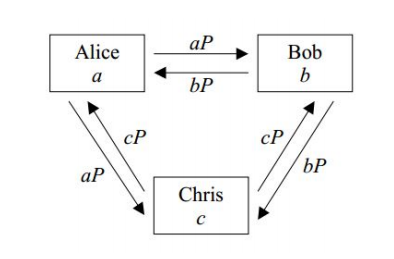
\includegraphics[width=0.65\linewidth]{../im22.png}
\caption{Trao đổi khóa}
\end{figure}
\end{center}
\subsubsection*{Truyền file}
Sau khi đã kí xác nhận và trao đổi khóa, đường truyền đã an toàn, người nhận file trực tiếp từ A thật sự đã là B chứ không phải kẻ tấn công, người gửi file cho B trực tiếp thật sự đã là A chứ không phải kẻ tấn công. Ta bắt đầu thao tác truyền file qua socket. 

Các hệ mã khóa đối xứng cho khả năng bảo mật cao hơn các hệ mã khóa công khai với cùng một kích thước khóa như nhau. Nói cách khác, các hệ mã khóa đối xứng cho thời gian tính toán nhanh hơn, hiệu quả hơn so với các hệ mã khóa công khai. Trong trường hợp truyền file bí mật giữa hai người, việc sử dụng các hệ mã khóa đối xứng với khóa đối xứng bí mật đã được thống nhất bởi thuật toán trao đổi khóa là tối ưu.

File được chuyển đi thông qua socket và được mã hóa theo chuẩn AES \index{AES}, tất cả hệ mã khóa đối xứng được cung cấp trong thư viên libsodium. Ở đây sử dụng hệ mã hóa khối AES-256-CTR
\begin{center}
\begin{figure}[H]
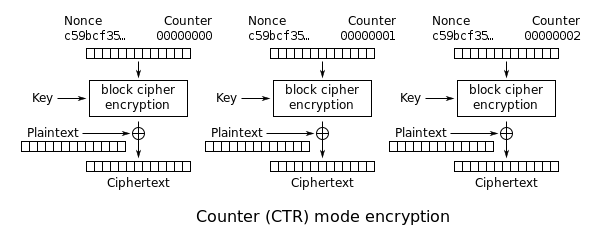
\includegraphics[width=0.9\linewidth]{../ctr-en.png}
\caption{Mã hoá AES-CTR}
\end{figure}
\end{center}
\begin{center}
\begin{figure}[H]
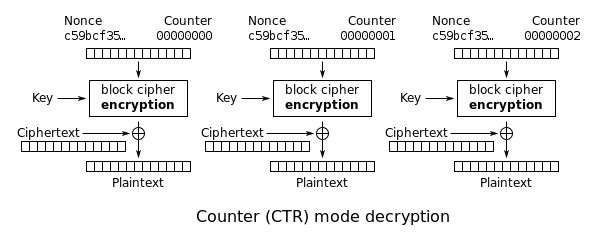
\includegraphics[width=0.9\linewidth]{../ctr-de.png}
\caption{Giải mã AES-CTR}
\end{figure}
\end{center}
\subsubsection*{Các kĩ thuật sử dụng}
\begin{itemize}
\item[1. ] Ngôn ngữ lập trình: C
\item[2. ] Thuật toán trao đổi khóa Diffie-Hellman dựa trên đường cong elliptic. Hàm add (cộng hai điểm), double(nhân đôi một điểm), inv (tính nghịch đảo), curve25519 được viết lại sử
dụng ngôn ngữ lập trình C và thư viện lbsodium để tăng tốc tính toán.
\item[3. ] Hệ chữ kí số Ed25519 do Daniel J. Bernstein đề xuất
\item[4. ] Hệ mã khóa đối xứng AES-256-CTR trong thư viện lbsodium.
\item[5. ] Thuật toán băm SHA-256 với sự hỗ trợ của thư viện Openssl
\item[6. ] Truyền dữ liệu qua socket.
\end{itemize}
\subsubsection*{Kết quả đạt được}
\begin{itemize}
\item[-] Xác nhận đối tượng tham gia chuyển file bằng chữ kí điện tử với khóa công khai.
\item[-] Thống nhất khóa đối xứng bí mật thành công nhờ thuật toán trao đổi khóa Diffie-Hellman dựa trên đường cong Curve25519.
\item[-] File được truyền đi bảo mật và nguyên vẹn.
\end{itemize}
\section{Chứng thư số ẩn}
\subsection*{Mục tiêu cơ bản}
\begin{itemize}
\item Xác thực danh tính giữa hai người giao tiếp A và B.
\item Sử dụng sơ đồ Elliptic Curve Qu-Vanstone Implicit Certificate Scheme (ECQV)
\item Chống lại tấn công MITM (Man In The Middle)
\end{itemize}
\subsection*{Các bước thực hiện}
\begin{itemize}
\item[1. ] Yêu cầu tạo chứng thư số ẩn(cả A và B đều yêu cầu tạo chứng thư số ẩn các bước yêu cầu tạo chứng thư đã được trình bày ở chương 3)
\item[2. ] Khi có chứng thư A và B thực hiện trao đổi khóa công khai với nhau(khóa công khai của A được trích rút từ chứng thư của A đưa cho B và khóa công khai của B được trích rút từ chứng thư của B đưa cho A như chương 3 đã trình bày)
\item[3. ] Khi có A và B đã có khóa công khai của nhau. Họ sẽ thực hiện trao đổi file với nhau như phần truyền file bí mật.
\end{itemize}
\subsubsection{Các kĩ thuật sử dụng}
\begin{itemize}
\item[•] Ngôn ngữ lập trình: C
\item[•] Thuật toán trao đổi khóa Diffe-Hellman trên đường cong Elliptic.
\item[•] Sơ đồ Elliptic Curve Qu-Vanstone Implicit Certificate Scheme (ECQV).
\item[•] Hàm băm SHA-256.
\item[•] Truyền file và chứng thư qua socket.
\end{itemize}
\subsubsection*{Kết quả đạt được}
\begin{itemize}
\item[-] Xác thực được danh tính người người tham gia giao tiếp giữa A và B.
\item[-] Thống nhất khóa đối xứng bí mật thành công nhờ thuật toán Elliptic Curve Qu-Vanstone Implicit và Diffe-Hellman.
\item[-] File được truyền đi bảo mật và nguyên vẹn.
\end{itemize}
\chapter*{Kết luận và hướng phát triển}
\section*{Kết quả đạt được}
Trong quá trình làm đồ án em đã đạt được những kết quả sau:
\begin{itemize}
\item[1. ] Tìm hiểu một số nguyên lý hệ mã công khai, hàm băm, chữ ký điện tử.
\item[2. ] Hiểu được lý thuyết về đường cong elliptic và một số kiến thức đại số trừu tượng liên quan áp dụng trong ngành mật mã học như nhóm và trường.
\item[3. ] Hiểu được các bước cơ bản để người ta xây dựng một đường cong ellitptic và ứng dụng của đường cong elliptic trong thuật toán trao đổi khóa và tạo chứng thư số ẩn.
\item[4. ] Nắm được một số kiểu tấn công vào các hệ mật mã như timing-attack \index{Timing-attack}, tấn công xen giữa (Man In The Middle).
\item[5. ] Xây dựng được ứng dụng chuyển file bí mật có các thao tác xác nhận (dùng hệ chữ kí điện tử ed25519) trao đổi khóa đối xứng bí mật (dùng thuật toán trao đổi khóa Diffie-Hellman dựa trên đường cong Curve25519).
\item[6. ] Xây dựng được ứng dụng chứng thư số ẩn với đường cong Twisted Edwards
\item[7. ] Có được cái nhìn vừa tổng quan, vừa chi tiết hơn về các hệ mật mã hiện đại.
\end{itemize}
\section*{Hạn chế}
Do hạn chế về thời gian hoặc (và) nhiều yếu tố chủ quan cũng như khách quan khác, đồ án vẫn còn một số hạn chế:
\begin{itemize}
\item[1. ] Chưa tìm hiểu được một cách đầy đủ và chi tiết về đường cong elliptic trên trường hữu hạn $\mathbb{F}_{2^m}$ với hai dạng cơ sở normal và polinomial.
\item[2. ] Vẫn còn rất nhiều phần kiến thức chưa tìm hiểu được như cách để tăng tốc độ tính toán của đường cong Curve25519 trên phần cứng cụ thể, lý do chi tiết giúp công thức cộng và nhân đôi Montgomery có thể chống lại được timing-attack \index{Timing-attack}, \ldots.
\item[3. ] Ứng dụng truyền file và chứng thứ số chưa có giao diện đẹp mắt và mới chỉ được kiểm thử trên một máy.
\end{itemize}
\section*{Hướng phát triển}
Do việc tính toán khóa trên đường cong elliptic là nhanh, việc lưu trữ và trao đổi khóa nhỏ gọn nên rất thích hợp cài đặt bảo mật cho các thiết bị IoT\index{IoT}(internet of thing) có bộ nhớ nhỏ khả năng tính toán thấp.

\begin{figure}[h]
\begin{subfigure}{.3\textwidth}
  \centering
  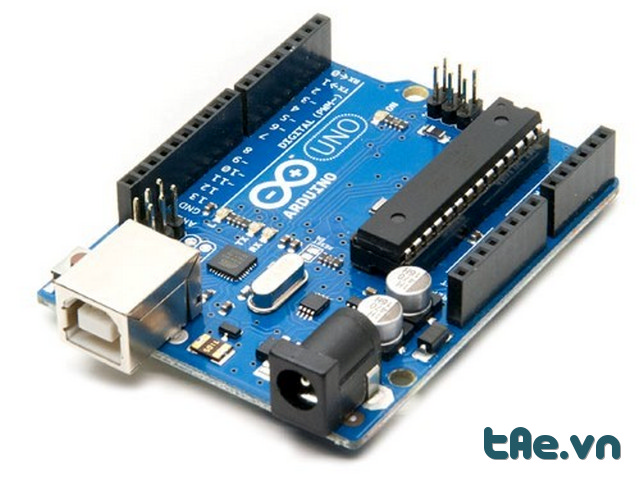
\includegraphics[width=1\linewidth]{../uno.jpg}
  %	\caption{1a elliptic trên trường số thực}
  \label{fig:sfig1}
\end{subfigure}%
\begin{subfigure}{.3\textwidth}
  \centering
  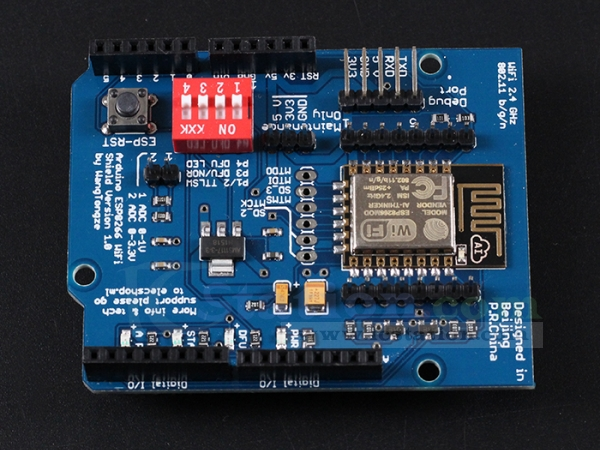
\includegraphics[width=1\linewidth]{../esp.jpg}
 % \caption{1b elliptic trên trường hưu hạn $\mathbb{F}_{29}$}
  \label{fig:sfig2}
\end{subfigure}
\begin{subfigure}{.3\textwidth}
  \centering
  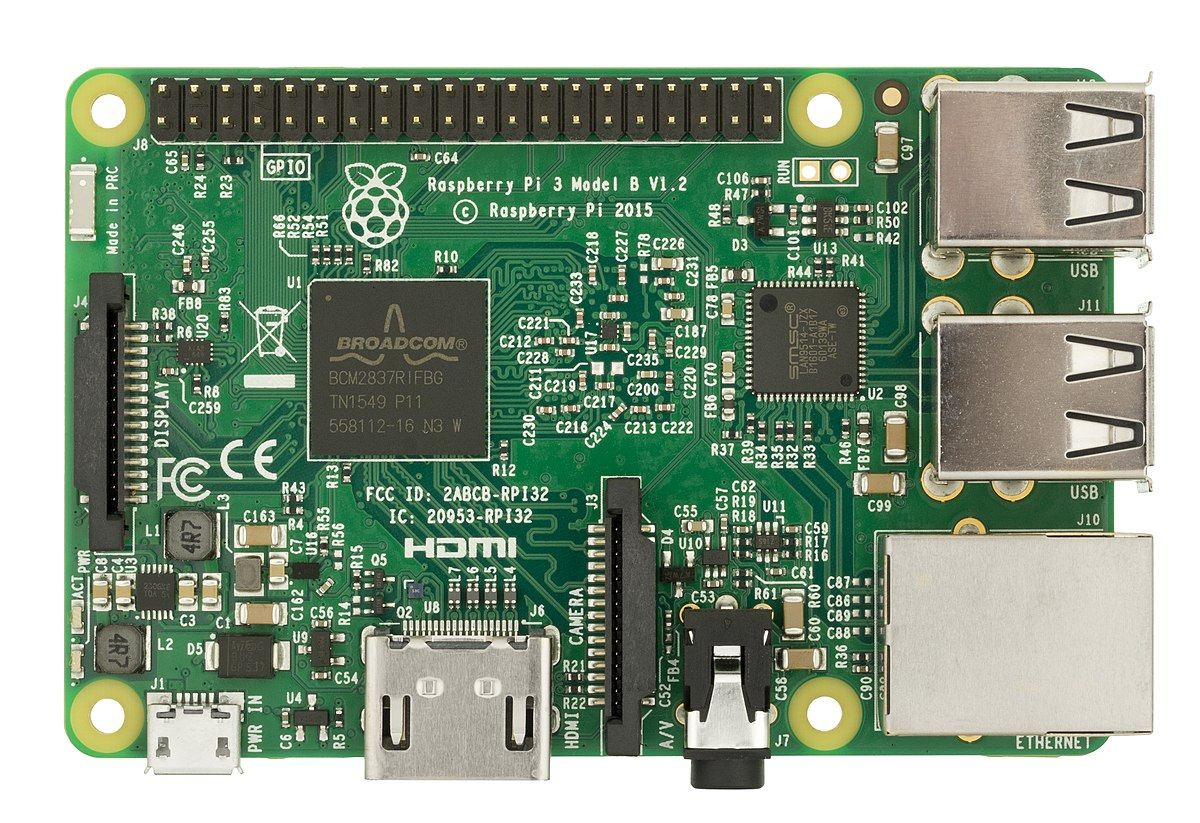
\includegraphics[width=1\linewidth]{../ras.jpg}
  \label{fig:sfig2}
\end{subfigure}
\caption{arduino, esp-12(esp8266), raspberry pi – các thiết bị dùng trong phát triển sản phẩm IoT} \label{h6.3}
\end{figure}

\printindex
\begin{thebibliography}{9}
\bibitem{csattt} Sách Giáo trình Cơ sở An toàn Thông tin thầy Nguyễn Văn Khanh - Đại học Bách Khoa.
\bibitem{Daninel} Daniel J. Bernstein. Cryptography in nacl, March 28 2012.
\bibitem{Daninel} Daniel J. Bernstein, Niels Duif, Tanja Lange, Peter Schwabe, and Bo-Yin Yang. \textit{High-speed high-security signatures}. Journal of Cryptographic Engineering, 2(2):77–89, 2012.
\bibitem{Daniel} Daniel J. Bernstein. \textit{Curve25519: New diffie-hellman speed records. In Public Key Cryptography - PKC 2006, 9th International Conference on Theory and Practice of Public-Key Cryptography}, volume 3958 of Lecture Notes in Computer Science, pages 207–228. Springer, 2006.
\bibitem{Jonathan} Jonathan Katz and Yehuda Lindell. \textit{Introduction to Modern Cryptography, Second Edition}. Chapman \& Hall/CRC,2\textsuperscript{nd} edition, 2014.
\bibitem{Standards for Efficient Cryptography} Certicom Research, \textit{SEC 1: Elliptic Curve Cryptography}, May 21-2009 version 2.0, \url{www.secg.org}.
\bibitem{Standards for Efficient Cryptography}Certicom Research, \textit{SEC 2: Recommended Elliptic Curve Domain Parameters}, Jan. 2010. Version 2.0. \url{www.secg.org}.
\bibitem{Standards for Efficient Cryptography} Certicom Research, \textit{SEC 4: Elliptic Curve Qu-Vanstone Implicit Certificate Scheme (ECQV)}. January 24, 2013. Version 1.0. \url{www.secg.org}
\bibitem{Undergraduate Texts in Mathematics}Jeffrey Hoffstein, Jill Pipher, Joseph H. Silverman, \textit{An Introduction to Mathematical Cryptography  Second Edition},  
\bibitem{book} Alfred J. Menezes, Scott A. Vanstone, and Paul C. Van Oorschot. \textit{Handbook of Applied Cryptography}. CRC Press, Inc., Boca Raton, FL, USA, 1\textsuperscript{st} edition, 1996.
\bibitem{article} Daniel J. Bernstein, Peter Birkner, Marc Joye, Tanja Lange and Christiane Peters, \textit{Twisted Edwards Curves}. Department of Mathematics, Statistics, and Computer Science (M/C 249) University of Illinois at Chicago, Chicago, IL 60607–7045, USA
\end{thebibliography}
\end{document}